%%%%%%%%%%%%%%%%%%%%%%%%%%%%%%
%%% Compile with LuaLaTeX! %%%
%%%%%%%%%%%%%%%%%%%%%%%%%%%%%%

% This must be in the first 5 lines to tell arXiv to use pdfLaTeX, which is strongly recommended.
% \pdfoutput=1
% In particular, the hyperref package requires pdfLaTeX in order to break URLs across lines.

\documentclass[11pt]{article}

% Change "review" to "final" to generate the final (sometimes called camera-ready) version.
% Change to "preprint" to generate a non-anonymous version with page numbers.
\usepackage[review]{acl}

% Standard package includes
% \usepackage{times}
% \usepackage{latexsym}

% For proper rendering and hyphenation of words containing Latin characters (including in bib files)
% \usepackage[T1]{fontenc}
% For Vietnamese characters
% \usepackage[T5]{fontenc}
% See https://www.latex-project.org/help/documentation/encguide.pdf for other character sets

% This assumes your files are encoded as UTF8
% \usepackage[utf8]{inputenc}

% This is not strictly necessary, and may be commented out,
% but it will improve the layout of the manuscript,
% and will typically save some space.
\usepackage{microtype}

% This is also not strictly necessary, and may be commented out.
% However, it will improve the aesthetics of text in
% the typewriter font.
\usepackage{inconsolata}

%Including images in your LaTeX document requires adding
%additional package(s)
\usepackage{graphicx}

% Custom packages
% \usepackage{lmodern}
\usepackage{fontspec}
\setmainfont{Times New Roman}
\defaultfontfeatures{Ligatures={TeX}}
\newfontfamily{\simplifiedchinesefont}{NotoSerifSC}
   \newcommand{\zh}[1]{\simplifiedchinesefont{#1}\rmfamily}

% \usepackage[fontset=PMingLiU]{ctex} % Disable default fontset
% \setCJKmainfont{} 
\usepackage{csquotes}
\usepackage{hyperref}
\usepackage{soul}
\usepackage{booktabs}
% \usepackage{dblfloatfix} % For fixing double column figures 

% If the title and author information does not fit in the area allocated, uncomment the following
%
%\setlength\titlebox{<dim>}
%
% and set <dim> to something 5cm or larger.

\title{Occupational gender bias in ungendered languages and LLMs: Comparing Hungarian and Chinese}

% Author information can be set in various styles:
% For several authors from the same institution:
% \author{Author 1 \and ... \and Author n \\
%         Address line \\ ... \\ Address line}
% if the names do not fit well on one line use
%         Author 1 \\ {\bf Author 2} \\ ... \\ {\bf Author n} \\
% For authors from different institutions:
% \author{Author 1 \\ Address line \\  ... \\ Address line
%         \And  ... \And
%         Author n \\ Address line \\ ... \\ Address line}
% To start a separate ``row'' of authors use \AND, as in
% \author{Author 1 \\ Address line \\  ... \\ Address line
%         \AND
%         Author 2 \\ Address line \\ ... \\ Address line \And
%         Author 3 \\ Address line \\ ... \\ Address line}

\author{First Author \\
  Affiliation / Address line 1 \\
  Affiliation / Address line 2 \\
  Affiliation / Address line 3 \\
  \texttt{email@domain} \\\And
  Second Author \\
  Affiliation / Address line 1 \\
  Affiliation / Address line 2 \\
  Affiliation / Address line 3 \\
  \texttt{email@domain} \\}

%\author{
%  \textbf{First Author\textsuperscript{1}},
%  \textbf{Second Author\textsuperscript{1,2}},
%  \textbf{Third T. Author\textsuperscript{1}},
%  \textbf{Fourth Author\textsuperscript{1}},
%\\
%  \textbf{Fifth Author\textsuperscript{1,2}},
%  \textbf{Sixth Author\textsuperscript{1}},
%  \textbf{Seventh Author\textsuperscript{1}},
%  \textbf{Eighth Author \textsuperscript{1,2,3,4}},
%\\
%  \textbf{Ninth Author\textsuperscript{1}},
%  \textbf{Tenth Author\textsuperscript{1}},
%  \textbf{Eleventh E. Author\textsuperscript{1,2,3,4,5}},
%  \textbf{Twelfth Author\textsuperscript{1}},
%\\
%  \textbf{Thirteenth Author\textsuperscript{3}},
%  \textbf{Fourteenth F. Author\textsuperscript{2,4}},
%  \textbf{Fifteenth Author\textsuperscript{1}},
%  \textbf{Sixteenth Author\textsuperscript{1}},
%\\
%  \textbf{Seventeenth S. Author\textsuperscript{4,5}},
%  \textbf{Eighteenth Author\textsuperscript{3,4}},
%  \textbf{Nineteenth N. Author\textsuperscript{2,5}},
%  \textbf{Twentieth Author\textsuperscript{1}}
%\\
%\\
%  \textsuperscript{1}Affiliation 1,
%  \textsuperscript{2}Affiliation 2,
%  \textsuperscript{3}Affiliation 3,
%  \textsuperscript{4}Affiliation 4,
%  \textsuperscript{5}Affiliation 5
%\\
%  \small{
%    \textbf{Correspondence:} \href{mailto:email@domain}{email@domain}
%  }
%}

\begin{document}

\maketitle

\begin{abstract}
This paper examines occupational gender bias and stereotypes in a cross-linguistic setting. We analyze ratings of 50 job titles collected from speakers of two languages without grammatical gender: Hungarian and Mandarin Chinese. Participants were instructed to rate how typical it is for a certain job to be associated with men or women, according to their own perceptions.
Our results show that in both languages the occupational nouns carry societal biases, despite the fact that the job titles themselves have no grammatical gender markings. We also analyze the ratings by participant gender and perform intra-linguistic and cross-linguistic comparisons, highlighting differences in the two languages and offering insights that range from peculiarities in word formation to broader cross-cultural generalizations.
Additionally, we compared the human raters' responses with that of a few popular generative AI agents. Interestingly, the biases exhibited by the LLMs in these chatbots were found to be even stronger than those shown by human participants.

\end{abstract}

\section{Introduction}

``Hairdressers are mostly women.'' -- one could say if during the course of their life they encountered more female than male hairdressers. But would this perception reflect reality? 
Occupational gender stereotypes are generalizations about the roles and characteristics of individuals in a certain group of in the workforce, and due to the long history of sex-based division of labour, it is one of the key components of gender stereotypes as a whole \citep{deaux_1984_structure}. Stereotypes are present from a young age \citep{canessapollard_2022_development} based on various inputs, such as personal observations, in-group--out-group bias, (social) media influence, societal norms and cultural narratives, and much more. As such, they are an inherent part of the human condition, originally said to be mechanism to make sense of biological sex differences \citep{levanon_2016_persistence}. These stereotypes are often prejudiced, inaccurate, and are ``misrepresenting the true ratios of gender in the workplace'' \citep{garnham_2015_true,gygax_2016_what} -- as \citet{kaukonen_2025_gender} have pointed out.

One of the factors in both shaping and reflecting social biases is language, and its role has been extensively studied in the past decades, including regarding occupational gender stereotypes \citep[cf.][]{sabatini_1985_occupational,pauwels_1997_handymen,gygax_2008_generically,misersky_2014_norms,lewis_2020_gender,kaukonen_2025_gender}. Much of the previous research have been conducted on languages with a grammatical gender system, such as Italian, French, German, Dutch, or English where occupational nomenclature and human agent nouns are often gendered (e.g., \textit{handyman}, \textit{seamstress}).\footnote{One important notion here is the asymetry between masculine and feminine forms of occupational nouns, that is, a lexical gap in occupational titles resulting in ``male as norm'' principle and the absence of words denoting a variety of female occupations \citep{baron_1986_grammar,hellinger_1990_kontrastive,sabatini_1985_occupational,yaguello_1978_mots,pauwels_2003_linguistic,lassonde_2013_occupational}.} 

% (((There is a counterexample for this phenomenon, in Arabic -- a Semitic language -- it would be considered ungrammatical to use the grammatically masculine form for any female individual pursuing an occupation.)))

% Observable instances for a binary set typical for Indo-European languages are for example French \textit{le coiffeur} vs. \textit{la coiffeuse} or German \textit{der Friseur} vs. \textit{die Friseurin} which are in accord with social genders, but we have instances for neutral forms as well, such as Dutch \textit{de kapper} (common gender) -- all meaning `hairdresser'.

In recent years, documentation of gender bias has been extented to other languages, such as Lithuanian, Icelandic, and Polish, also including languages without grammatical gender like Chinese, Japanese, and Thai \citep[][]{hellinger_2003_gender,pauwels_2003_linguistic}. Most recently, \citet{kaukonen_2025_gender} compared Estonian and Russian, where the former lacks grammatical gender.

Our study compares Hungarian and Chinese, both of which lack grammatical gender, which in turn does not mean that these languages are free of gender biases. We are interested in how speakers of these two languages navigate the stereotypes of the workplace and how much they impose gender biases present in society onto jobs and occupational titles without explicit gender markings.

\subsection{Background}

\subsubsection{Hungarian}

Hungarian is a Finno-Ugric language in the Uralic language family, without a grammatical gender system,\footnote{The problematics of linguistic gender in Hungarian has been discussed by \citet{vasvari_2014_problemas}.} and most occupational nouns and job titles are realized in linguistically gender-neutral terms. 
On the surface level, the feminine form is created by appending \textit{-nő} `woman' to the unmarked base word, but in reality, these female-marked nouns are formed by compounding \textit{nő} `woman' (a noun) to the base word (noun or adjective), which is a regular way of producing female occupational titles. In practice however, this does not equal to a symmetric male-female pair, as the unmarked form is not necessarily ``masculine'', it is also neutral. We can observe 3 types in the pragmatic usage of occupational nouns when it comes to the unmarked--marked pairing and its implications for the gendering of the unmarked nouns at the discourse level:

\textbf{1) Both forms are common.} Frequently occuring word-pairs in Hungarian would be for example \textit{énekes} `singer' -- \textit{énekesnő} `female singer' (not in our dataset). In cases where both occur with a relatively high frequency in a balanced corpus -- the unmarked word seems to carry some male bias, as the frequent use of a feminine form indicates a need and/or custom for differentiation. We wanted to test if raters perceived this type of bias or not. In this example, the absolute and relative frequencies (occurrance per a million words) of the two lemmatized nouns in the Hungarian National Corpus (HNC) are 1441/9.4001 for \textit{énekes} and 748/4.8795 for \textit{énekesnő} \citep{varadi_2002_hungarian, oravecz_2014_hungarian}; the frequency difference here is roughly half (51.9\%).

The striking deviations in frequencies for marked--unmarked word pairs such as the above are not an indicator for a strong perceptual gender bias -- we can assume that both men and women singers would be equally represented in the Hungarian corpus -- but reflect that in general, the unmarked, neutral forms are used for either males or females when talking about one's occupation. The female-marked forms are used when there is an explicit intention to specify the gender of the individual, and when it is otherwise not known from context or from proper names.\footnote{For example, the sentence \textit{Anyukám tanár.} is the canonical way of saying `My mom is a teacher.'. It uses the unmarked form, primarily because we want to channel information about the individual's vocation, and secondly because it is obvious from the subject that she is a woman, so the marking would be redundant.} A special situation would be the use of the vocative case, which requires the marked form when addressing female professionals, e.g., \textit{Tanárnő!} `teacher (f.)' or \textit{Doktornő!} `doctor (f.)'.

\textbf{2) Only unmarked form is common.} There are many cases where the unmarked form is the only one generally used for both genders. Take for example \textit{ügyész} `prosecutor' (8451/55,1287) vs. \textit{ügyésznő} `female prosecutor' (56/0,3653), or \textit{fodrász} `hairdresser' (944/6.1580) vs. \textit{fodrásznő} `female hairdresser' (35/0.2283); the deviations in frequency here are over multiple orders of magnitude. In these instances, the unmarked form is the default word to describe anyone practicing the occupation regardless of gender, and appending \textit{'-nő} `woman' to it -- although possible -- would render it unusual and a bit awkward; but still not as uncanny as Modern English \textit{singress} would be.\footnote{Although English had a form \textit{singeress} from Middle English, it is now obsolete.}

\textbf{3) Marked form is common.} Some female-marked terms ending in \textit{-nő} are ubiquitous, making the unmarked version a bit unusual, such as \textit{házvezető} `housekeeper' (10/0.0652) vs. \textit{házvezetőnő} `female housekeeper' (92/0.6001), or, to a small extent \textit{takarító} `cleaner' (169/1.1024) vs. \textit{takarítónő} `female cleaner' (392/2.5571). In our opinion these instances reflect deeply engrained societal biases.

\subsubsection{Chinese}

Chinese, a Sino-Tibetan language, marks gender only when writing the 3rd person singular pronoun (\zh{他} \textit{tā} `he' / \zh{她} \textit{tā} `she') but that too is a relatively recent invention, going back to the May Fourth Movement of 1919 \citep{bi_2013_tazi}, and similarly to Hungarian, most occupations are unmarked for gender.

% \hl{New from Wenhui from here...}

% In Chinese, occupational titles are primarily formed through compound word formation, with their semantic core focused on describing the work content, function, or domain rather than directly denoting the gender of the practitioner. Regarding the morphological patterns of Chinese occupational compounds, scholars have proposed various classification methods \citep{packard_2000_morphology,fu_2014_chinese}. Among these, the `head + quasi-suffix' derivational pattern represents one of the most predominant models \citep{fu_2014_chinese}. These quasi-suffixes typically denote specific identities or categories of people, functionally analogous to suffixes like `-er', `-ian' or `-ist' in English, but retain a degree of semantic substance without complete grammaticalization \citep{fu_2014_chinese}. Examples include \zh{师} \textit{shī} in \zh{教师} \textit{jiaòshī} `teacher' and \zh{工程师} \textit{gōngchéngshī} `engineer', \zh{家} \textit{jiā} in \zh{科学家} \textit{kēxuéjiā} `scientist' and \zh{画家} \textit{huàjiā} `painter', and \zh{员} in \zh{服务员} \textit{fúwùyuán} `waiter/waitress'. While these morphemes possess independent lexical meanings, such as \zh{师} denoting `military division' and \zh{家} meaning `home/residence', their quasi-suffixal derivation shows in the formation of occupational nouns. Another significant pattern is the `verb-object' (V-O) compound \citep{packard_2000_morphology}, which directly describes the core action of the work and its object. For instance, in \zh{编剧} \textit{biānjù} `playwright/screenwriter', \zh{编} (\textit{verb}: `to organize; create') governs \zh{剧} (\textit{noun}: `drama; script') as its object. Similar structures include \zh{司机} \textit{sījī} `driver'(\zh{司}: \textit{v}.: `to operate; control' + \zh{机}: \textit{n}.: `machine/vehicle') and \zh{保安} \textit{baǒān} `security guard' (\zh{保} \textit{v}.: `to protect' + \zh{安}, \textit{n}., `safety'). Furthermore, Chinese occupational titles incorporate loanwords, such as \zh{模特} \textit{mótè}, from French \textit{modèle} or English \textit{model}, and \zh{博客} \textit{bōkè}, from English \textit{blogger}. Upon entering Chinese, these terms typically conform to native morphological habits and usage rules, and their forms likewise carry no grammatical gender information.

Chinese is generally acknowledged as a language that lacks grammatical gender from a structural perspective \citep{li_1989_mandarin}. In contrast to languages with mandatory noun gender systems such as French, or German, Chinese nouns and adjectives lack gender distinctions. Thus, certain scholars contend that the Chinese linguistic system is fundamentally gender-neutral and may not inherently reflect gender classification \citep{li_1989_mandarin,packard_2000_morphology}.

Nonetheless, sociolinguistic research argues that language use, particularly at the pragmatic level, is significantly shaped by socio-cultural attitudes \citep{labov_1972_sociolinguistic}, and many occupations are associated with relatively strong gender stereotypes \citep{sun_1997_language,su_2021_occupational}. For instance, \zh{护士} \textit{hùshì} `nurse' and \zh{保姆} \textit{báomǔ} `nanny', are predominantly female occupations, whereas \zh{警察} \textit{jǐngchá} `police officers' and \zh{高管} \textit{gāoguǎn} `executive; manager', are predominantly male roles. This societal perception results in pragmatic asymmetry: although occupational terms are grammatically gender-neutral, speakers or language users frequently form default gender assumptions in communication contexts based on societal stereotypes. Consequently, when a practitioner's gender diverges from the conventional stereotype associated with their profession, or when particular circumstances require explicit gender identification, speakers often precede occupational terms with gender markers \zh{男} \textit{nán} for `male' or \zh{女} \textit{nǚ} for `female', such as \zh{男护士} \textit{nánhùshì} for `male nurse', \zh{女警察} \textit{nǚjǐngchá} for `female police officer', \zh{女高管} \textit{nǚgāoguǎn} for `female executive', and \zh{男保姆} \textit{nánbáomǔ} for `male nanny'. This practice of incorporating gender markers demonstrates a dual effect \citep{sun_1997_language,gustafssonsenden_2015_introducing,su_2021_occupational}. On one hand, it emphasises the transcendence of gender constraints by individuals, thereby increasing the visibility of specific groups, particularly those in non-traditional gender roles. Conversely, this gender-focused terminology may, particularly in contradictory contexts, reinforce prevailing gender stereotypes \citep{sun_1997_language,gustafssonsenden_2015_introducing}. For instance, under societal cognition specific to China, the aforementioned occupation title \zh{高管} \textit{gāoguǎn} `executive' subconsciously defaults to a male referent. Highlighting \zh{女高管} \textit{nǚgāoguǎn} `female executive' designates the individual as an anomaly and may inadvertently maintain the gender stereotype in China that associates the term `executive' predominantly with males, showing an intrinsic uniqueness or necessity for explicit distinction when women assume this position.

In summary, Chinese occupational titles are inherently gender-neutral, due to the lack of grammatical gender and their primary function of solely describing the work itself. The addition of gender modifiers such as \zh{男} \textit{nán} `male' or \zh{女} \textit{nǚ} `female' operates as a pragmatic device rather than a grammatical requirement. This strategy primarily signals socio-cognitive markedness by highlighting deviations from occupation-gender stereotypes (i.e., denoting non-prototypical associations), as empirically demonstrated in Chinese corpora where terms like \zh{女总统} \textit{nǚzóngtǒng}, `female president' occur more frequently than their male-marked counterparts in leadership roles \citep{su_2021_occupational,farris_1988_gender}. Concurrently, it fulfills referential specificity in contexts demanding explicit gender identification, such as legal depositions or medical documentation where deixis resolution is pragmatically necessary \citep{hellinger_2003_gender,stahlberg_2011_representation}.

% \hl{...to here.}

Regarding both languages, we are interested in the unmarked occupational nouns, as they do not inherently possess linguistic gender bias, but according to our expectations they can reflect prevailing societal stereotypes, and thus show varying degrees of gender bias. Our research questions are: 
\begin{itemize}
  \item To what extent do speakers of Hungarian and Chinese exhibit gender bias when rating occupations and job titles?
  \item Are there significant in gender bias between male and female raters within the same language?
  \item What are the key differences and similarities in occupational gender stereotypes between Hungarian and Chinese speakers?
\end{itemize}

Moreover, in recent years, with the advent of Large Language Models (LLMs), the challenge of addressing occupational gender stereotypes has been a prominent issue in language technology as well \citep[cf.][]{kirk_2021_bias,ju_2024_female,an_2025_mutual}. To see how LLMs handle gender biases compared to human participants, we also conducted a series of experiments using the LLMs of popular artificial intelligence (AI) companies and analyzed their outputs, both in Hungarian and Chinese.

% In section \ref{sec:experiment_setup} we describe the experimental setup and our methods of analysis, followed by the results and their discussion in section \ref{sec:results}. Finally, we look at how AI compares to human raters in section \ref{sec:ai_comparison}.

\section{Experimental setup}\label{sec:experiment_setup}

For both languages we designed a survey-based experiment in which participants were asked to rate job titles on a 7-point Likert scale, ranging from \textit{completely male} (-3) to \textit{completely female} (+3). Participants were instructed to decide on how likely is an occupation to be pursued by men or by women.\footnote{While this study focuses on people who identify or are identified as either male or female, we acknowledge the presence of non-binary people in the workforce.}

\subsection{Participants}

% \begin{figure}[!ht]
%   \centering
%   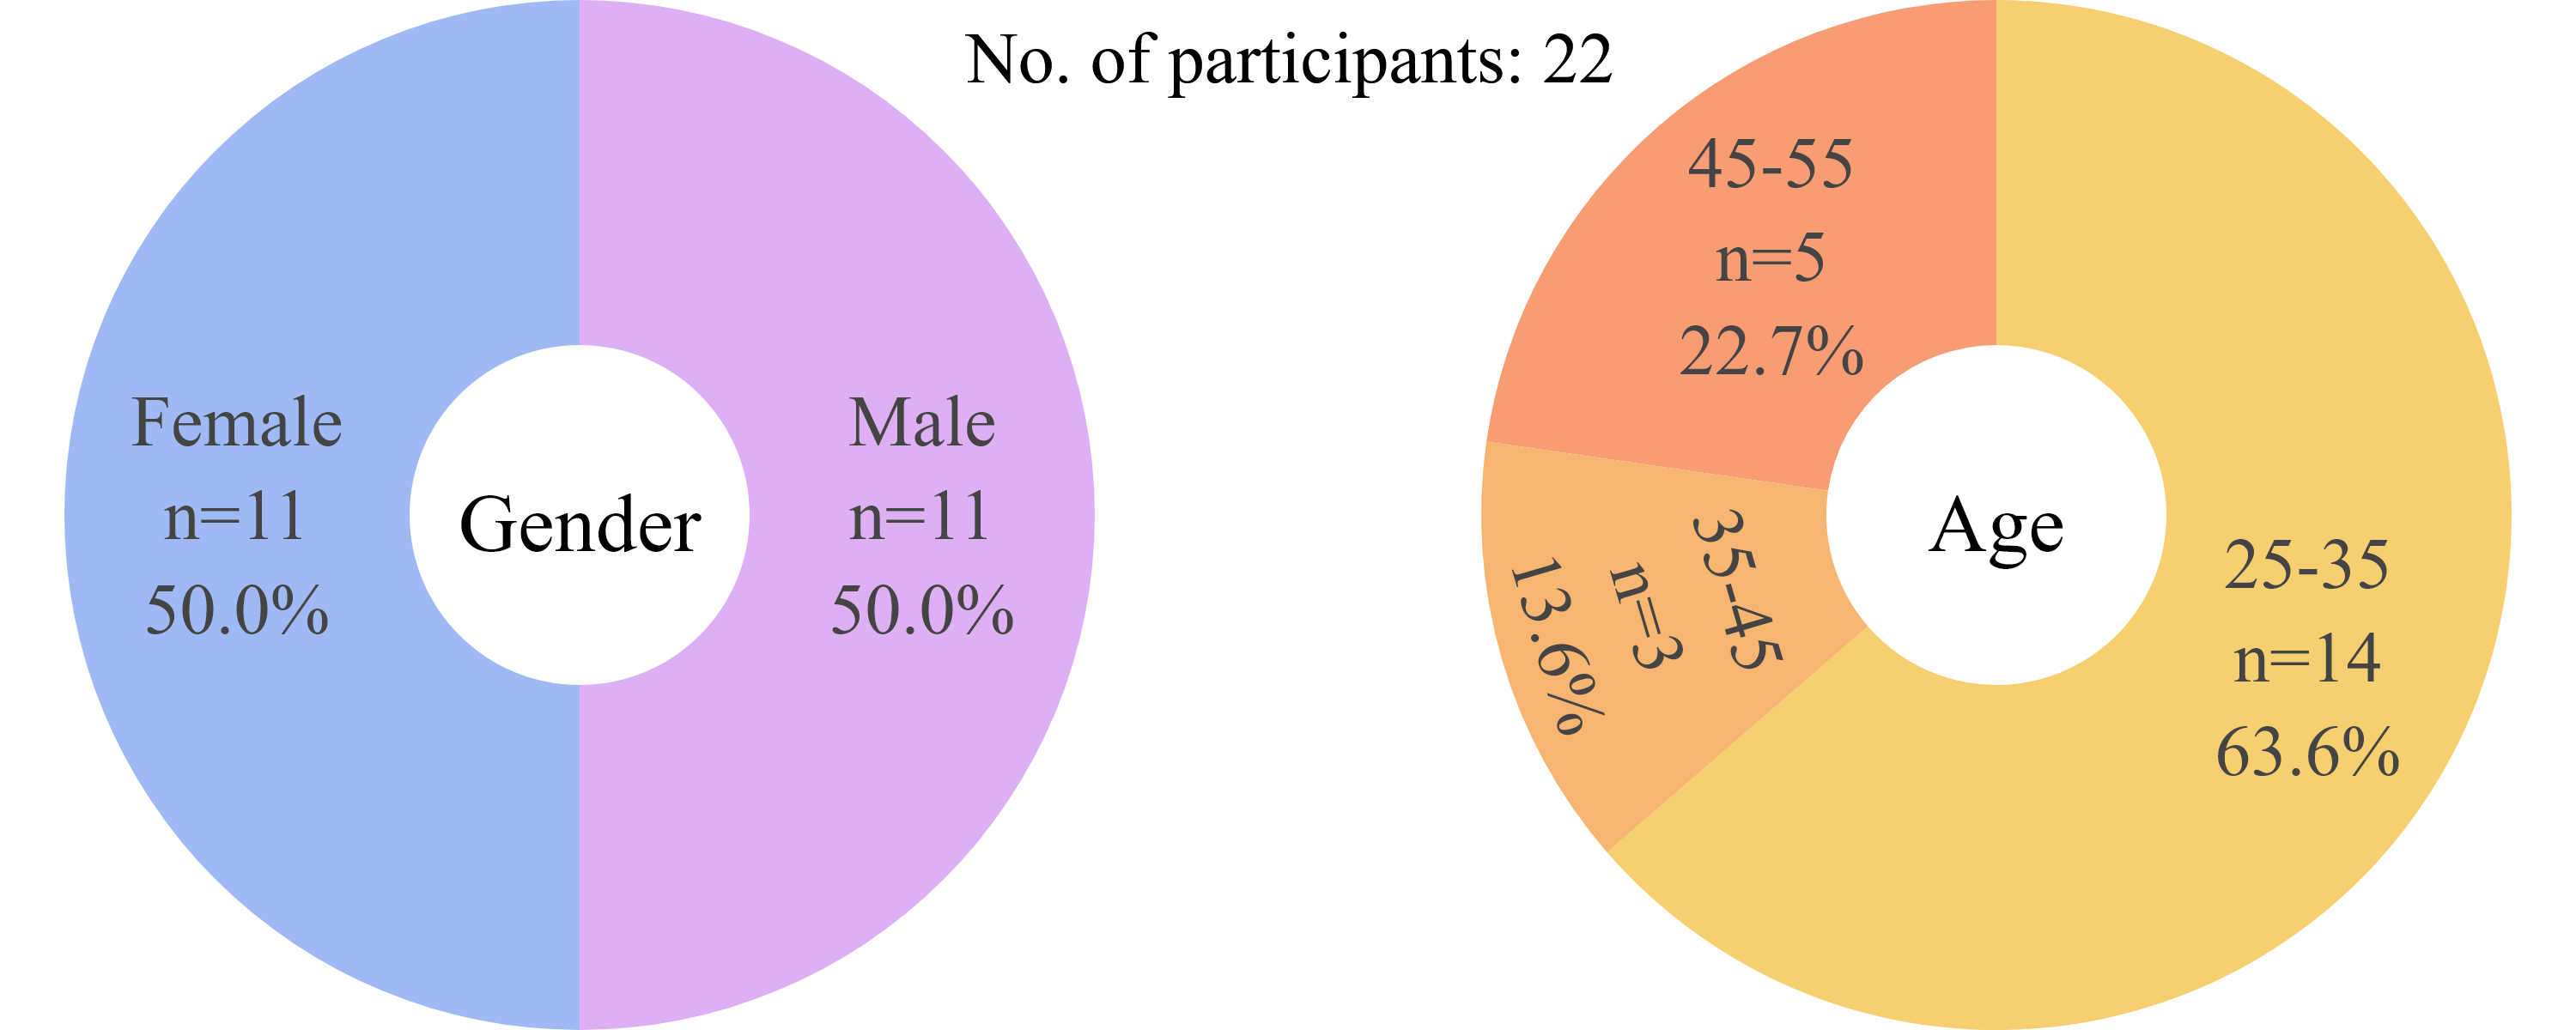
\includegraphics[width=\linewidth]{../demographics_hu}
%   \caption{Demographics of the Hungarian participants.}
%   \label{fig:demographics_hu}
% \end{figure}

A total of 24 native Hungarian speakers filled our questionnaire, and after validating the responses (reviewing attention checks and any anomalies) 2 were rejected. Participants were recruited online using Prolific (https://www.prolific.com/), with screeners set for location (Hungary) and first language (Hungarian); raters were compensated for their time with a small monetary reward. In the end, the Hungarian dataset had 22 participants (11 female), with age-ranges of 25-35 (n=14), 35-45 (n=3), and 45-55 (n=5) for formal analysis. See Figure~\ref{fig:demographics_hu} for the distribution.

% \begin{figure}[!ht]
%   \centering
%   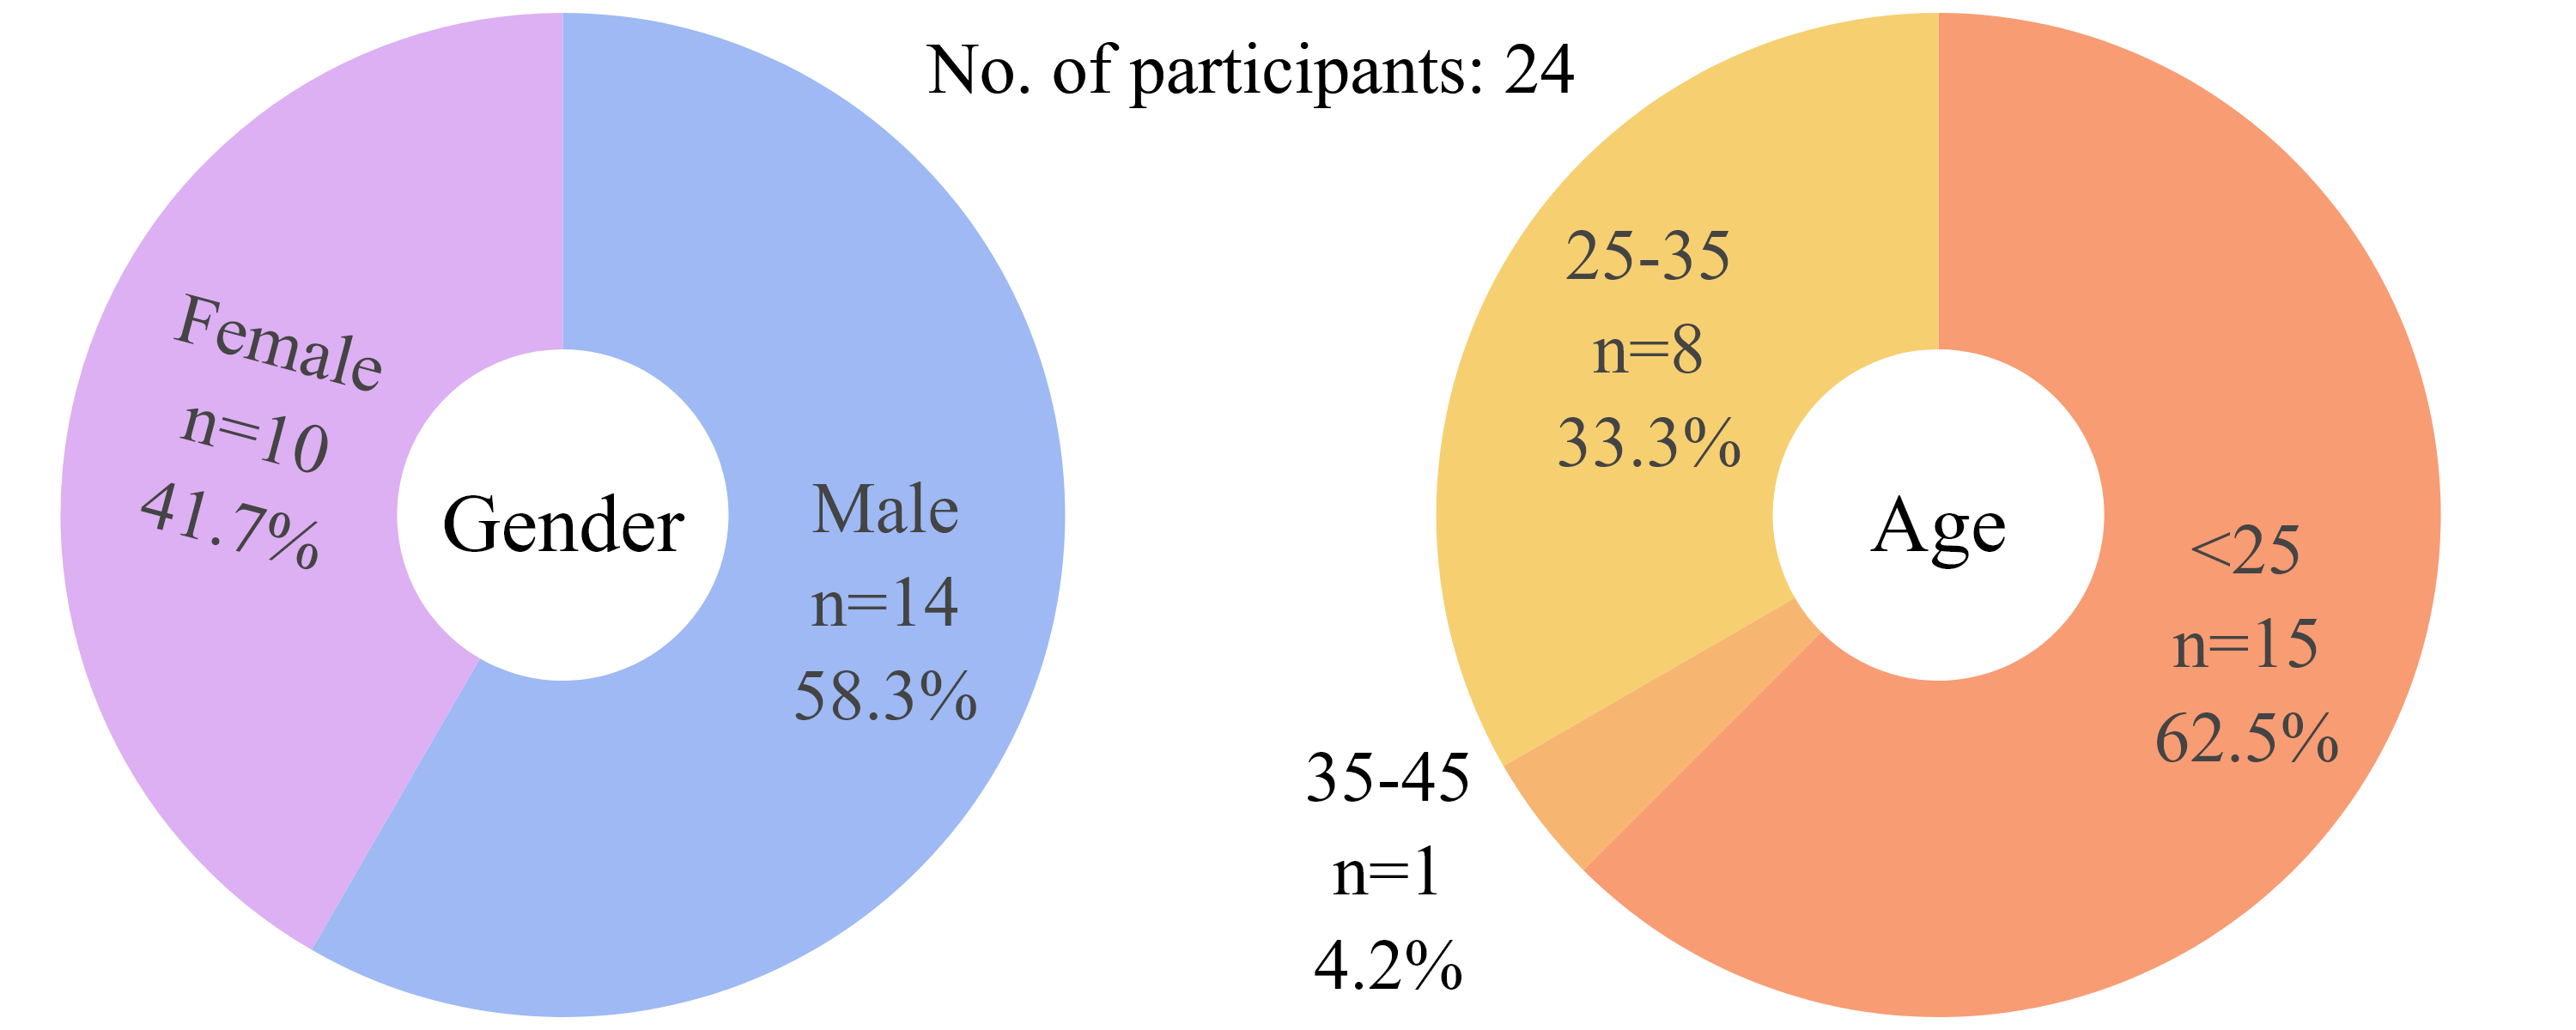
\includegraphics[width=\linewidth]{../demographics_zh}
%   \caption{Demographics of the Chinese participants.}
%   \label{fig:demographics_zh}
% \end{figure}

The Chinese survey was completed by 30 native Mandarin Chinese speakers, 6 of which were rejected after attention checks. Chinese participants were recruited from career development interest groups on WeChat, and they were required to have been born and raised in mainland China and with Mandarin as their primary language and the primary language spoken at home. Additionally, they must have resided in China continuously for the past five years. Participants were paid a small fee for completing the questionnaire. The 24 accepted participants (10 female) were mostly university students, aged <25 (n=15), 25-35 (n=8), or 35-45 (n=1). See Figure~\ref{fig:demographics_zh} for the distribution.

\subsection{Materials}

The Hungarian survey contained 44 items (see Appendix \ref{sec:hungarian_items}) and 6 attention-check items, each a well-known occupational title in Hungary, such as: \textit{modell} `model' or \textit{katona} `soldier'. The attention-check items were removed from the final analysis, these were \textit{pincérnő} `waitress', \textit{titkárnő} `secretary (female)', \textit{tanárnő} `teacher (female)', \textit{takarítónő} `cleaning lady', \textit{ápolónő} `nurse (female)', and \textit{házvezetőnő} `housekeeper (female)'. These words explicitly determine the gender of the worker and all should be rated `completely female' (3). Participants who rated any of these lower than 2, or rated them lower than 3 more then once were rejected.

The 6 words above have counterparts without the \textit{nő} `woman' element, e.g., \textit{pincér} `waiter', and all were included in our survey. As explained, these words are unmarked for gender, but they do not explicitly refer to men. Therefore, the expected gender bias in the ratings of these occupations -- if any -- is more likely to be due to social factors, not linguistic ones.\footnote{We have included \textit{diák} `student' out of curiosity. Although being a student is not a job per se, but it is beyond doubt the only truly gender-neutral ``occupation'' there is, since it is mandatory for everyone to go to school (both in Hungary and in China). We wanted to see if there would be any bias regarding this word, especially that Hungarian has a female-marked form for it -- \textit{diáklány} `girl student', adding \textit{-lány} `girl' to the base noun -- and could be considered to belong to the 1st type with a potential male bias when considered in contrast.}

The Chinese survey contained 44 items of commonly occurring job titles in Mandarin Chinese shown in Simplified Chinese characters (see Appendix \ref{sec:chinese_items}), with 6 attention checks. The attention checks were \zh{妈妈} \textit{māmā} `mother', \zh{爸爸} \textit{bàba} `father', \zh{女作家} \textit{nǚzuòjiā} `female writer', \zh{男作家} \textit{nánzuòjiā} `male writer', \zh{女画家} \textit{nǚhuàjiā} `female painter', \zh{男画家} \textit{nánhuàjiā} `male painter'. These words are inherently feminine or masculine in meaning, or explicitly determine gender by prepending \zh{女} \textit{nǚ} `woman' and \zh{男} \textit{nán} `man', helping to filter out inattentive responses. Participants who failed to rate these with the highest scores of either \textit{completely male} or \textit{completely female} were rejected.

The two wordlists were not exactly the same, only 41 of the 44 occupational nouns overlap.

\subsubsection{Procedure}

Hungarian and Chinese participants were both instructed to rate each word between \textit{completely male} and \textit{completely female}, the ratings were then converted to numerical values from -3 to +3. Hence, the choices were completely male (-3); mostly male (-2); somewhat male (-1); neutral/equal (0); somewhat female (+1); mostly female (+2); completely female (+3). The exact wording of the main question of the Hungarian survey was: ``Ön szerint a foglalkozás tipikusan férfi foglalkozás, vagy tipikusan női foglalkozás?'' (Is this occupation typically a man's occupation or a woman's occupation?), while in Chinese it was: ``\zh{对于\hspace{0pt}XX\hspace{0pt}这个职业,\hspace{0pt}您\hspace{0pt}认为\hspace{0pt}通常\hspace{0pt}担\hspace{0pt}任该\hspace{0pt}职业\hspace{0pt}的\hspace{0pt}男女\hspace{0pt}性别\hspace{0pt}比例\hspace{0pt}是\hspace{0pt}多少?}'' (What do you think is the ratio of men to women in \_\_?). 
The surveys were created in Microsoft Forms with essentially identical instructions. Hungarian participants were presented with the words in a list format in no particular order without context, each word with a corresponding rating scale next to it (cf. Fig. \ref{fig:survey_hu}), Chinese participants saw each word highlighted in a question above, and were presented with the scale directly below, in a random order (cf. Fig. \ref{fig:survey_zh}). Time limit was not set, but the survey was designed to take around 5 minutes, and participants have finished under 5 minutes on average.

In addition to the surveys by native speakers, we have prompted 5 different popular AI chatbots: Mistral AI's Le Chat (Free), Microsoft's Copilot (+Think Deeper), OpenAI's ChatGPT (GPT-5 Preview), DeepSeek (Deepthink R1), and Google's Gemini (2.5 Flash), to elicit ratings on the same job titles. In both languages we used the same scale, the same instructions with a pretext: ``You are participating in an experiment and your answers will help our research.''.\footnote{See the instructions \href{https://anonymous.4open.science/r/occupational-gender-bias/instructions_hu.txt}{here (HU)} and \href{https://anonymous.4open.science/r/occupational-gender-bias/instructions_zh.txt}{here (ZH)}.} Between August 7 and 14, 2025 we have prompted each AI agent 10 different times (2×5×10=100 total prompts), and then aggregated the results.\footnote{The raw data is available \href{https://anonymous.4open.science/r/occupational-gender-bias/occupations.xlsx}{here}.}

\subsection{Methods}

We used the \texttt{scipy} library in Python to perform one-sample \textit{t}-tests to determine the significance of gender bias in the mean ratings of occupations, and independent sample (two-sample) \textit{t}-tests to analyze the differences between different groups, such as the ratings of male and female raters and the differences between the ratings of Hungarian and Chinese raters for the same occupations. When comparing the ratings of humans with AI systems, we performed Pearson's correlation to determine the strength of the relationship between the ratings and determine which LLM is more aligned with human judgments. 

For the sake of reproducibility and open science, we have made the data and code available in this repository: \href{https://anonymous.4open.science/r/occupational-gender-bias}{https://anonymous.4open.science/r/occupational-gender-bias}, where all files and procedures (\texttt{main.ipynb}) are available.

\section{Results \& Discussion}\label{sec:results}

For both languages, the majority of occupations were rated with a significant gender bias (\textit{p}<0.05), measured against 0 (neutral/equal). In Hungarian 36 out of 44 occupations showed significant bias, in Chinese 40 out of 44.

\subsection{Hungarian}

% \begin{figure*}[!ht]
%   \centering
%   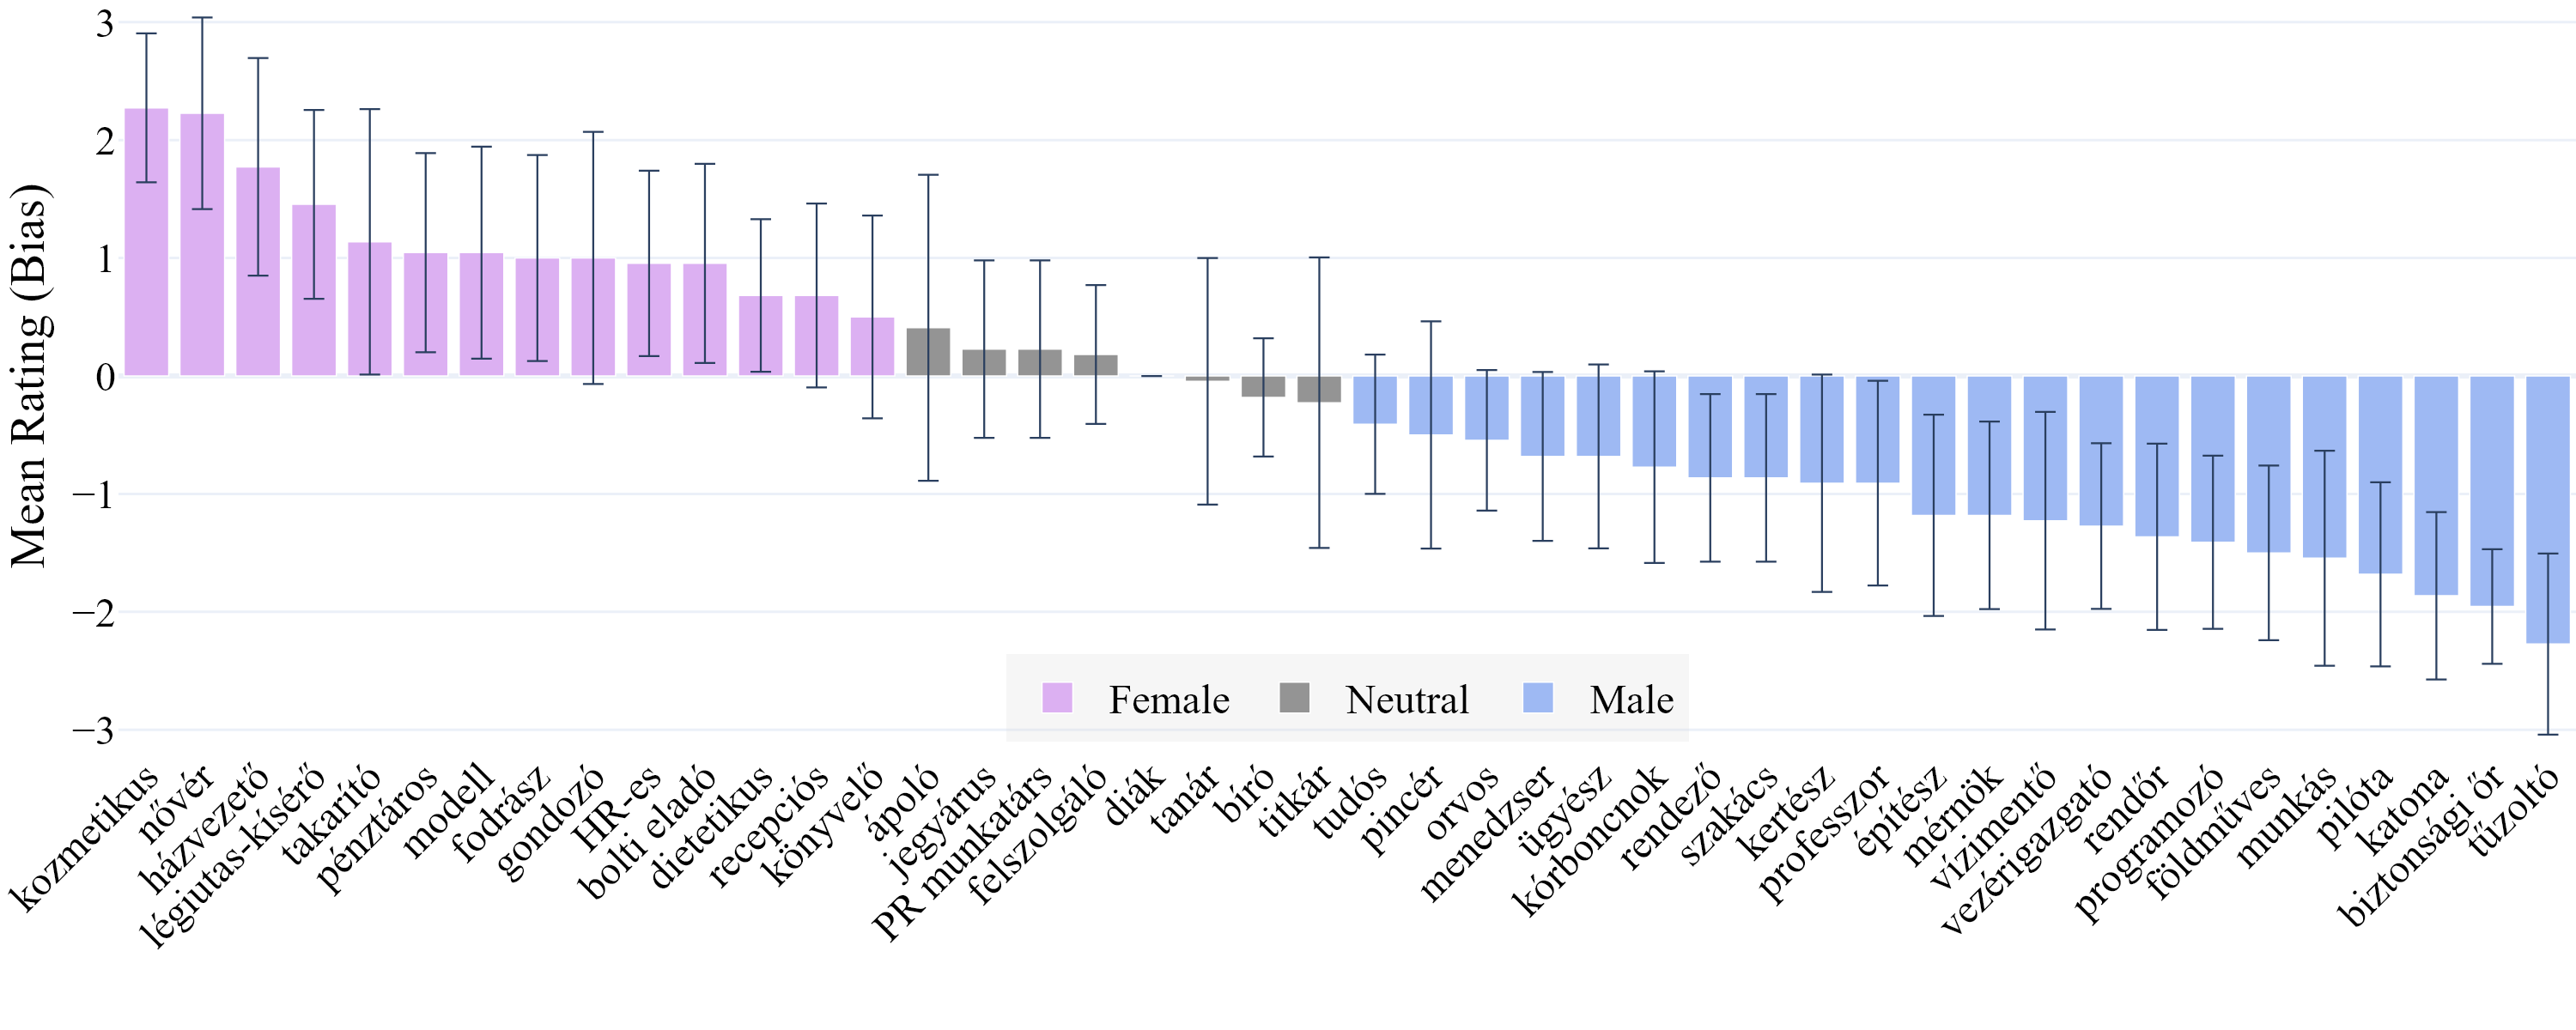
\includegraphics[width=\linewidth]{../occupations_hu}
%   \caption{Mean ratings of occupational titles in Hungarian with standard deviations, significant gender bias highlighted -- \href{https://anonymous.4open.science/api/repo/occupational-gender-bias/file/occupations_hu.html?v=93359859}{explore the interactive plot}.}
%   \label{fig:occupations_hu}
% \end{figure*}

% \begin{figure*}[tbp]
%   \centering
%   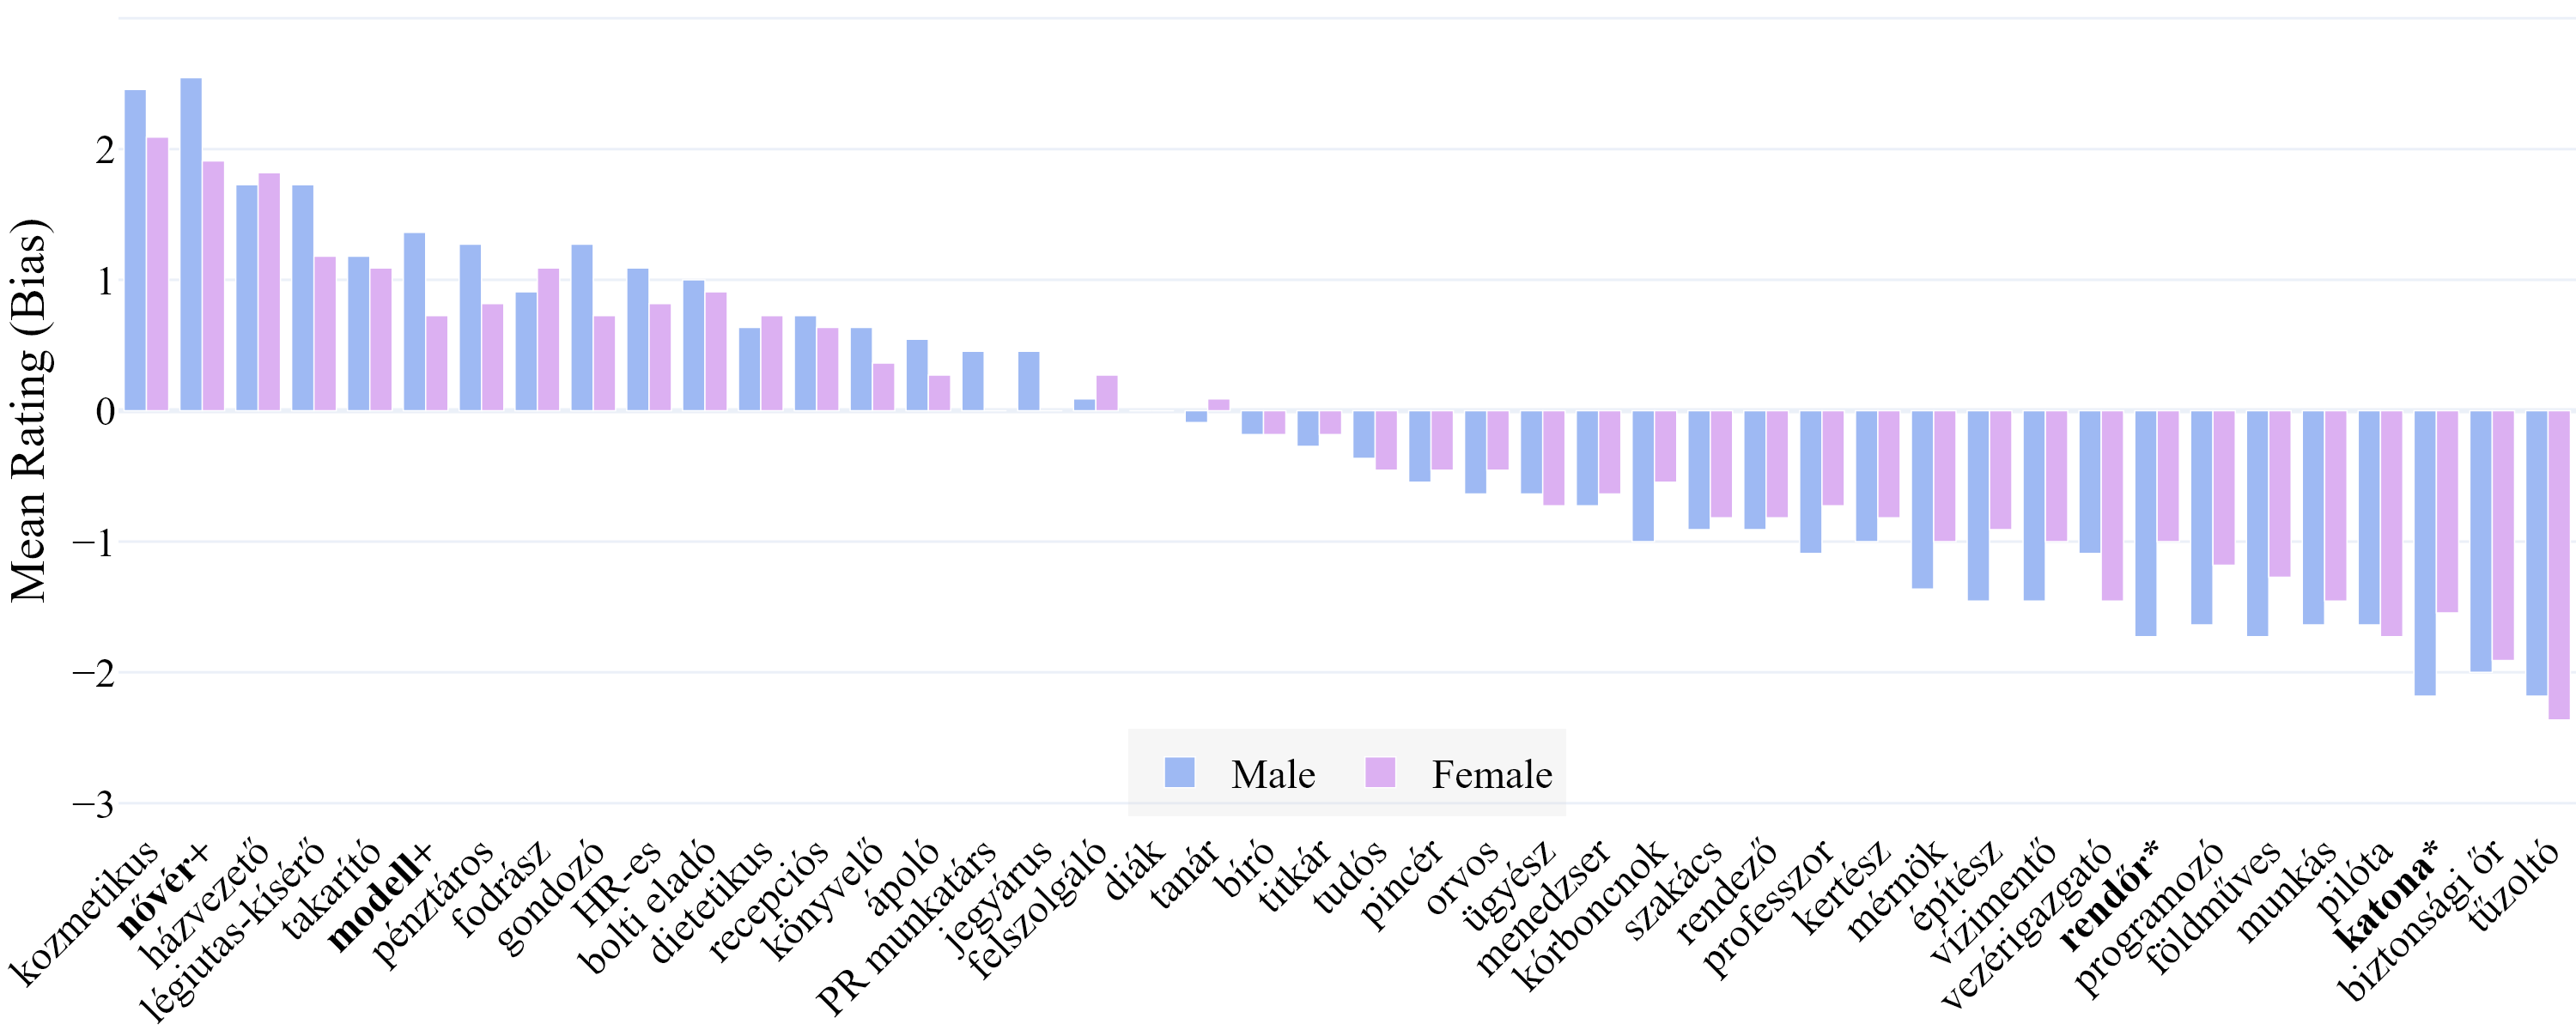
\includegraphics[width=\linewidth]{../occupations_hu_gender}
%   \caption{Mean ratings of occupational titles in Hungarian by gender, significant differences highlighted (significant*, and marginally significant+ in \textbf{bold}) -- \href{https://anonymous.4open.science/api/repo/occupational-gender-bias/file/occupations_hu_gender.html?v=cf836c31}{explore the interactive plot}.}
%   \label{fig:occupations_hu_gender}
% \end{figure*}

According to the Hungarian ratings, among the 36 occupational titles rated with a significant gender bias, 14 showed female, and 22 showed male bias. See Figure \ref{fig:occupations_hu} in the Appendix for a visualization of the mean ratings with the biases highlighted.

\subsubsection{Overall distribution of ratings}

In general, occupations were rated according to expectations, following societal stereotypes, disregarding the grammatically unmarked nature of the words. The top 5 terms with the highest female bias were \textit{kozmetikus} `beautician' (2.27), \textit{nővér} `nurse' (2.23),\footnote{\textit{Nővér} `nurse' (2.23) -- is a bit special, as it literally means `sister' and goes back to the time when nuns were the ones taking care of the sick; hence the word carries a strong female bias that is encoded in its literal meaning. Interestingly, it was not rated as an exclusively female job, probably because male nurses are now also common. The gender-neutral word \textit{ápoló} `nurse' for the same job was also tested, and it received a neutral rating of 0.41.} \textit{házvezető} `housekeeper' (1.77), \textit{légiutas-kísérő} `flight attendant' (1.45), and \textit{takarító} `cleaner' (1.14), while the top 5 terms with the highest male bias were \textit{tűzoltó} `firefighter' (-2.27), \textit{biztonsági őr} `security guard' (-1.95), \textit{katona} `soldier' (-1.86), \textit{pilóta} `pilot' (-1.68), and \textit{munkás} `worker' (-1.55). Notice the high number of service-jobs on the female side.

% Table with two subtables about the top words with the highest female bias, and a table with the highest male bias with 3 columns: word, gloss, score.

% \begin{table}
%   \label{}
%   \centering
%   \begin{tabular}{lcr}
%     \toprule
%     \textbf{Word} & \textbf{Gloss} & \textbf{Score} \\
%     \midrule
%     \textit{kozmetikus} & beautician & 2.27 \\
%     \textit{nővér} & nurse & 2.23 \\
%     \textit{házvezető} & housekeeper & 1.77 \\
%     \textit{légiutas-kísérő} & flight attendant & 1.45 \\
%     \textit{takarító} & cleaner & 1.14 \\
%     \midrule
%     \textit{tűzoltó} & firefighter & -2.27 \\
%     \textit{biztonsági} őr & security guard & -1.95 \\
%     \textit{katona} & soldier & -1.86 \\
%     \textit{pilóta} & pilot & -1.68 \\
%     \textit{munkás} & worker & -1.55 \\
%     \bottomrule
%   \end{tabular}
% \end{table}

The 8 job titles that came back as not biased were: \textit{ápoló} `nurse' (0.41), \textit{jegyárus} `ticket seller' (0.23), \textit{PR munkatárs} `PR specialist' (0.23), \textit{felszolgáló} `server' (0.18),  \textit{diák} `student' (0), \textit{tanár} `teacher' (0), \textit{bíró} `judge' (-0.18), and \textit{titkár} `secretary' (-0.23). It is worth noting that while \textit{diák} `student' was rated 0 by everyone, \textit{tanár} `teacher' had more individual variation in the ratings.

The strongest agreement between raters were on \textit{diák} `student' (0, std=0), \textit{biztonsági őr} `security guard' (-1.95; std=0.4857), \textit{bíró} `judge' (-0.18; std=0.5011), \textit{felszolgáló} `server' (0.18; std=0.5885), \textit{tudós} `scientist' (-0.41; std=0.5903).

\subsubsection{Intra-language gender differences}

We also compared the ratings of male and female participants for each occupation, to see if there was any discrepancies between the two groups. The only jobs that showed a significant difference was \textit{rendőr} `police officer' (men: -1.73; women: -1.00) and \textit{katona} `soldier' (men: -2.18; women: -1.55), here the male biases were much higher by male raters. These results are summarized in Figure \ref{fig:occupations_hu_gender}.

Furthermore, these results suggest that men tend to have a greater absolute bias for both male- and female-coded jobs (see Figure \ref{fig:confusion_matrices} in the Appendix).



\subsection{Chinese}

% \begin{figure*}[!ht]
%   \centering
%   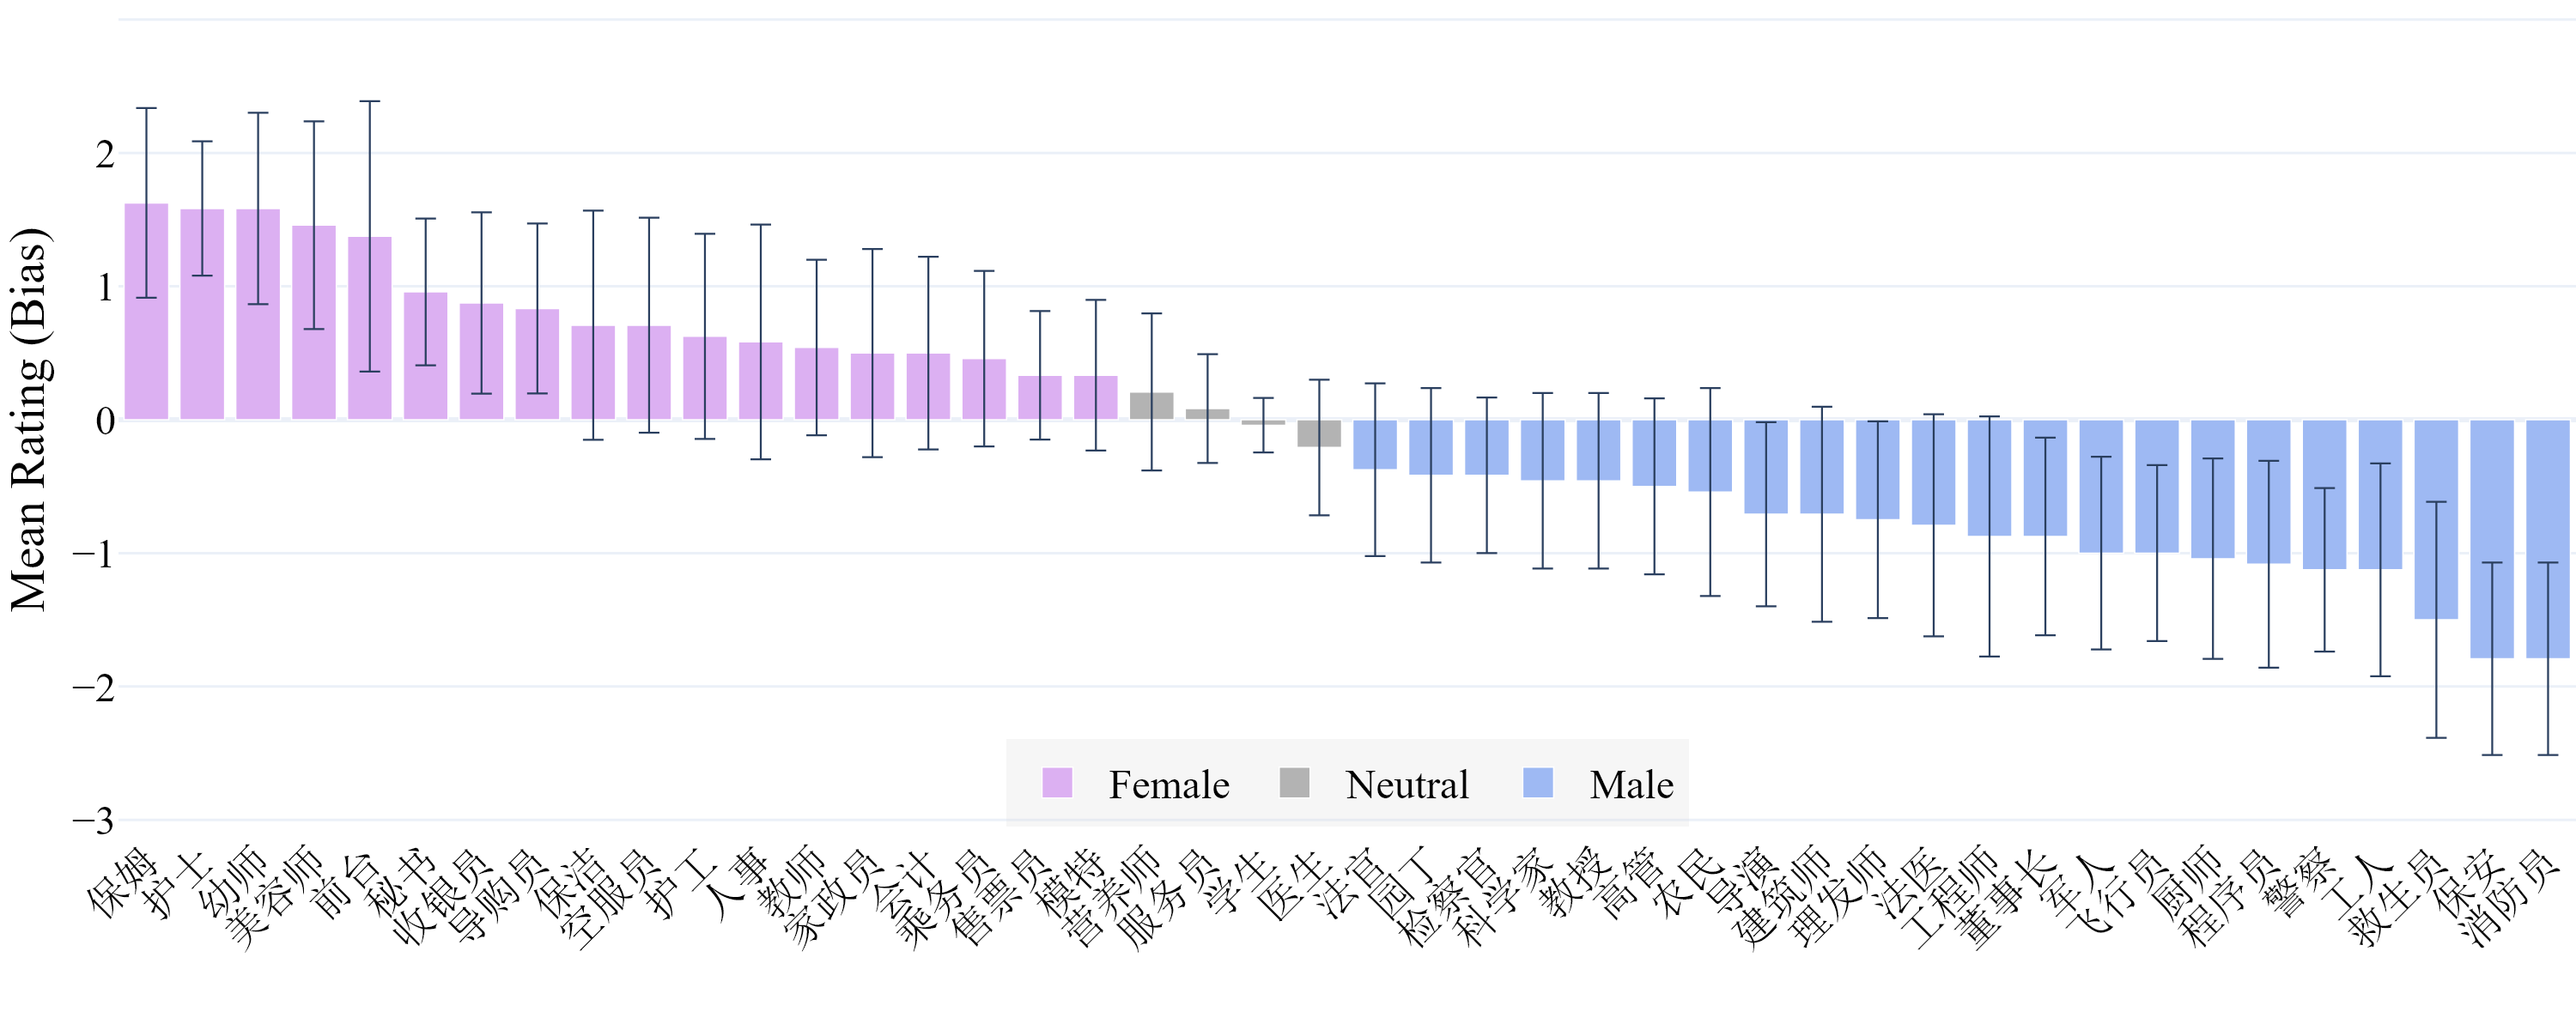
\includegraphics[width=\linewidth]{../occupations_zh}
%   \caption{Mean ratings of occupational titles in Chinese with standard deviations, significant differences highlighted -- \href{https://anonymous.4open.science/api/repo/occupational-gender-bias/file/occupations_zh.html?v=9fe887c1}{explore the interactive plot}.}
%   \label{fig:occupations_zh}
% \end{figure*}

% \begin{figure*}[tbp]
%   \centering
%   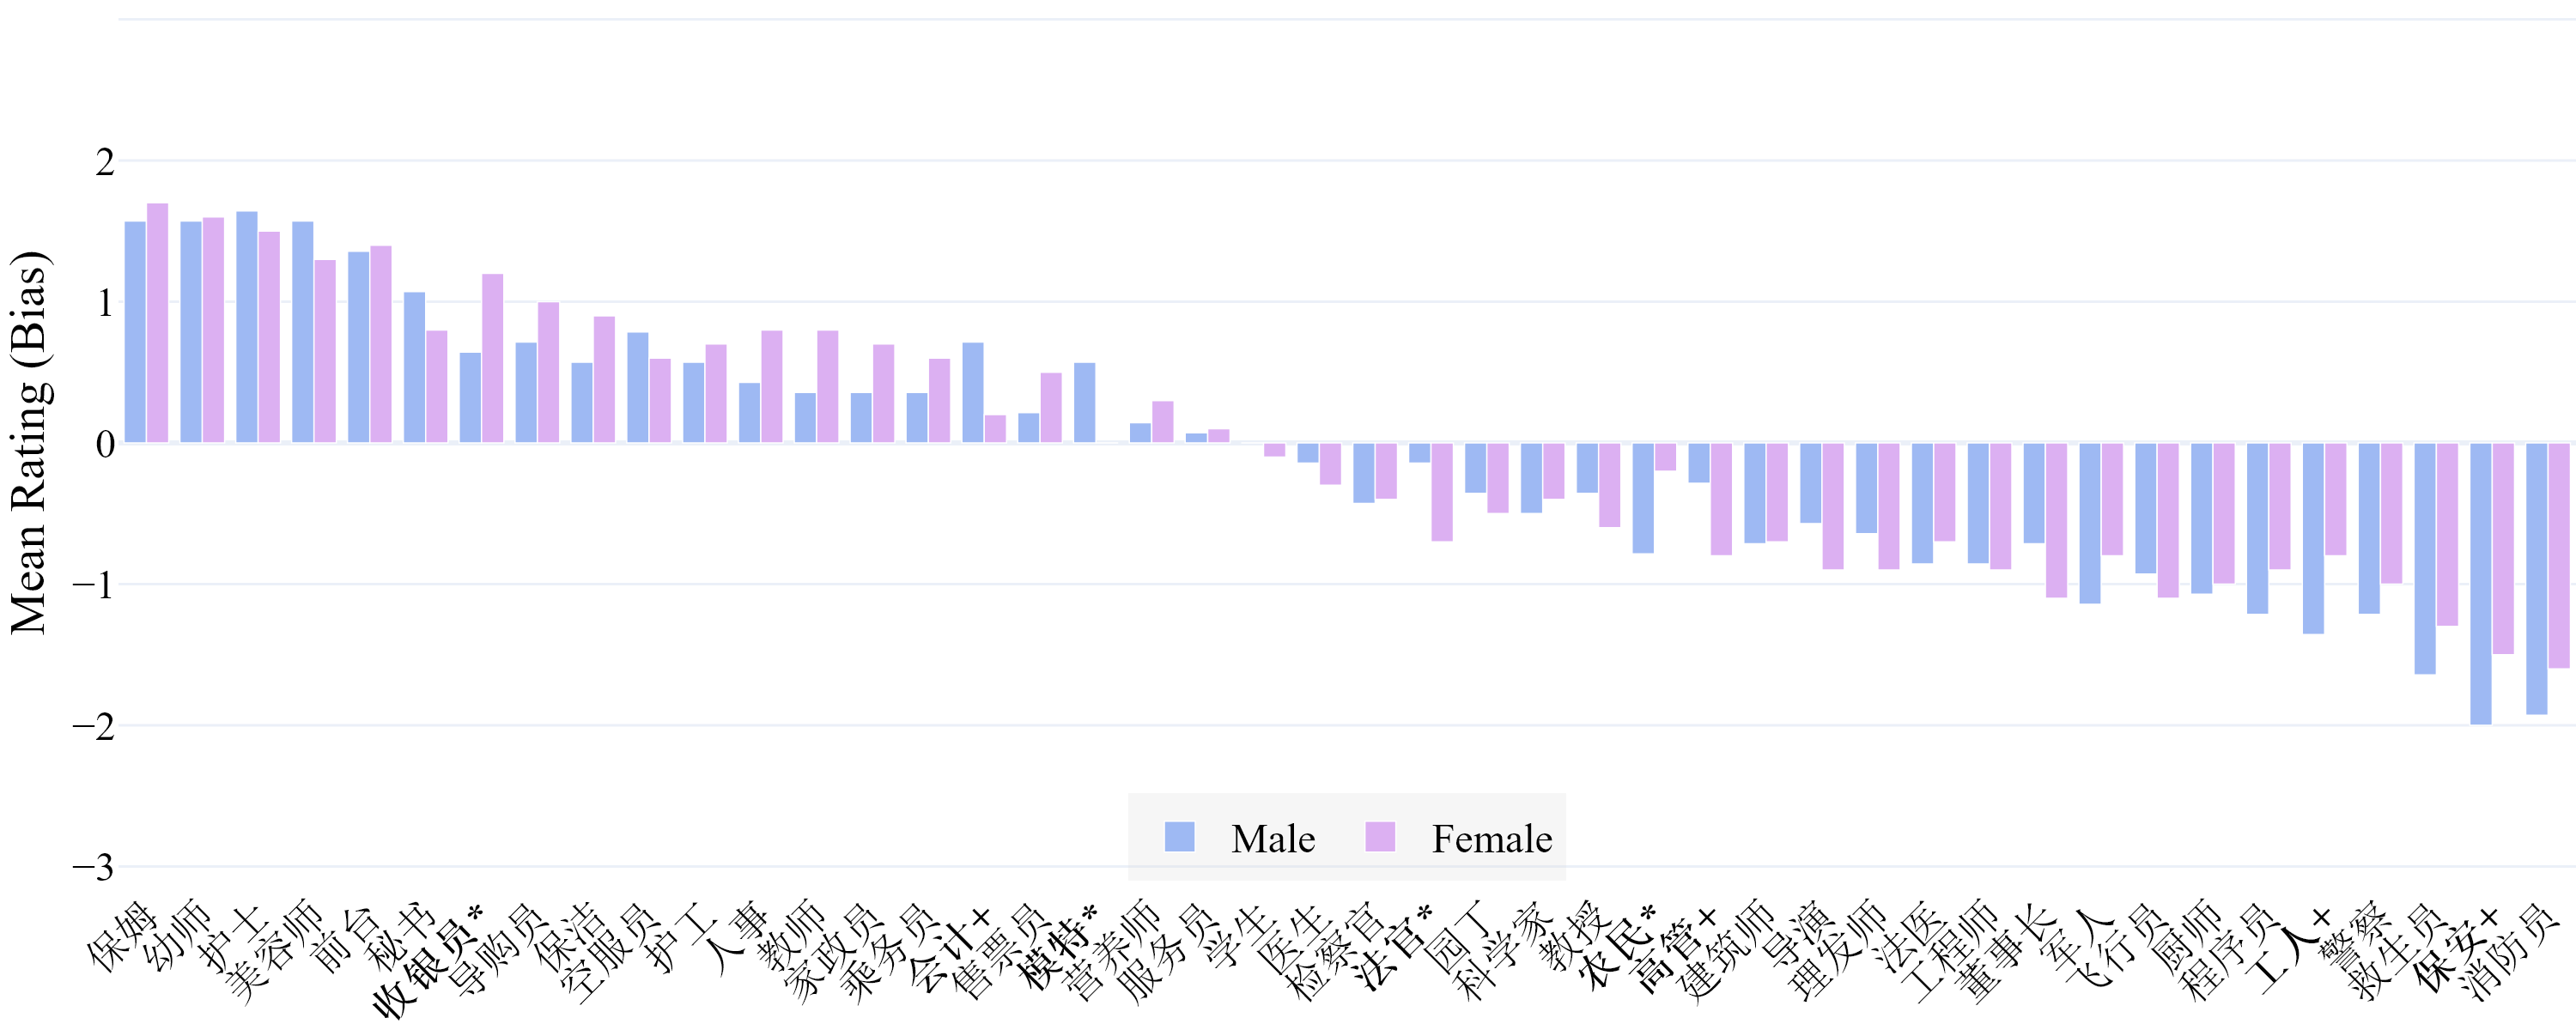
\includegraphics[width=\linewidth]{../occupations_zh_gender}
%   \caption{Mean ratings of occupational titles in Chinese by gender, significant differences highlighted (significant*, and marginally significant+ in \textbf{bold}) -- \href{https://anonymous.4open.science/api/repo/occupational-gender-bias/file/occupations_zh_gender.html?v=99428eda}{explore the interactive plot}.}
%   \label{fig:occupations_zh_gender}
% \end{figure*}

The analysis of Chinese ratings showed that out of the 40 significantly biased occupations, 18 revealed female bias, and 22 male bias. Ratings are shown in Figure \ref{fig:occupations_zh}.

\subsubsection{Overall distribution of ratings}

% \hl{New from Wenhui from here...}

The rating results largely aligned with our expectations concerning occupational gender stereotypes in Chinese society, participants typically linked women to childcare, emotional labor, and service-oriented roles while associating men with high-intensity, high-risk physical labor, and order-maintaining roles.

% \hl{...to here}

In our results, the words with the highest female bias were \zh{保姆} `domestic helper' (1.63), \zh{护士} `nurse' (1.58), \zh{幼师} `kindergarten teacher' (1.58), \zh{美容师} `beautician' (1.46), and \zh{前台} `receptionist' (1.38). Words with the highest male bias were \zh{消防员} `firefighter' (-1.79), \zh{保安} `security guard' (-1.79), \zh{救生员} `lifeguard' (-1.50), \zh{工人} `worker' (-1.13), and \zh{警察} `police officer' (1.13) which shows a relatively strong similarity to the Hungarian trends.

% Table with two subtables about the top words with the highest female bias, and a table with the highest male bias with 3 columns: word, gloss, score.

% \begin{table}
%   \label{tab:occupations_zh}
%   \centering
%   \begin{tabular}{lcr}
%     \toprule
%     \textbf{Word} & \textbf{Gloss} & \textbf{Score} \\
%     \midrule
%     \zh{保姆} & nanny & 1.63 \\
%     \zh{护士} & nurse & 1.58 \\
%     \zh{幼师} & kindergarten teacher & 1.58 \\
%     \zh{美容师} & beautician & 1.46 \\
%     \zh{前台} & receptionist & 1.38 \\
%     \midrule
%     \zh{消防员} & firefighter & -1.79 \\
%     \zh{保安} & security guard & -1.79 \\
%     \zh{救生员} & lifeguard & -1.50 \\
%     \zh{工人} & worker & -1.13 \\
%     \zh{警察} & police officer & -1.13 \\
%     \bottomrule
%   \end{tabular}
% \end{table}

The 4 neutral job titles without bias were: \zh{营养师} `dietitian' (0.21), \zh{服务员} `waiter/server' (0.08), \zh{学生} `student' (-0.04), and \zh{医生} `doctor' (-0.21). While `student' is almost equal here as well, in Chinese \zh{教师} `teacher' (0.54) appeared on the female side. 

Consistent with Hungarian results, Chinese data also showed a strong agreement on \zh{学生} `student' (-0.04; std=0.2041) and \zh{服务员} `waiter/server' (0.08; std=0.4082), the remaining words in the top 5 jobs with the lowest standard deviation (=strongest agreement) were \zh{售票员} `ticket seller' (0.33; std=0.4815), \zh{护士} `nurse' (1.58; std=0.5036), and \zh{医生} `doctor' (-0.21; std=0.5089).

% Maybe can delete from above.

% \begin{figure*}[!ht]
%   \centering
%   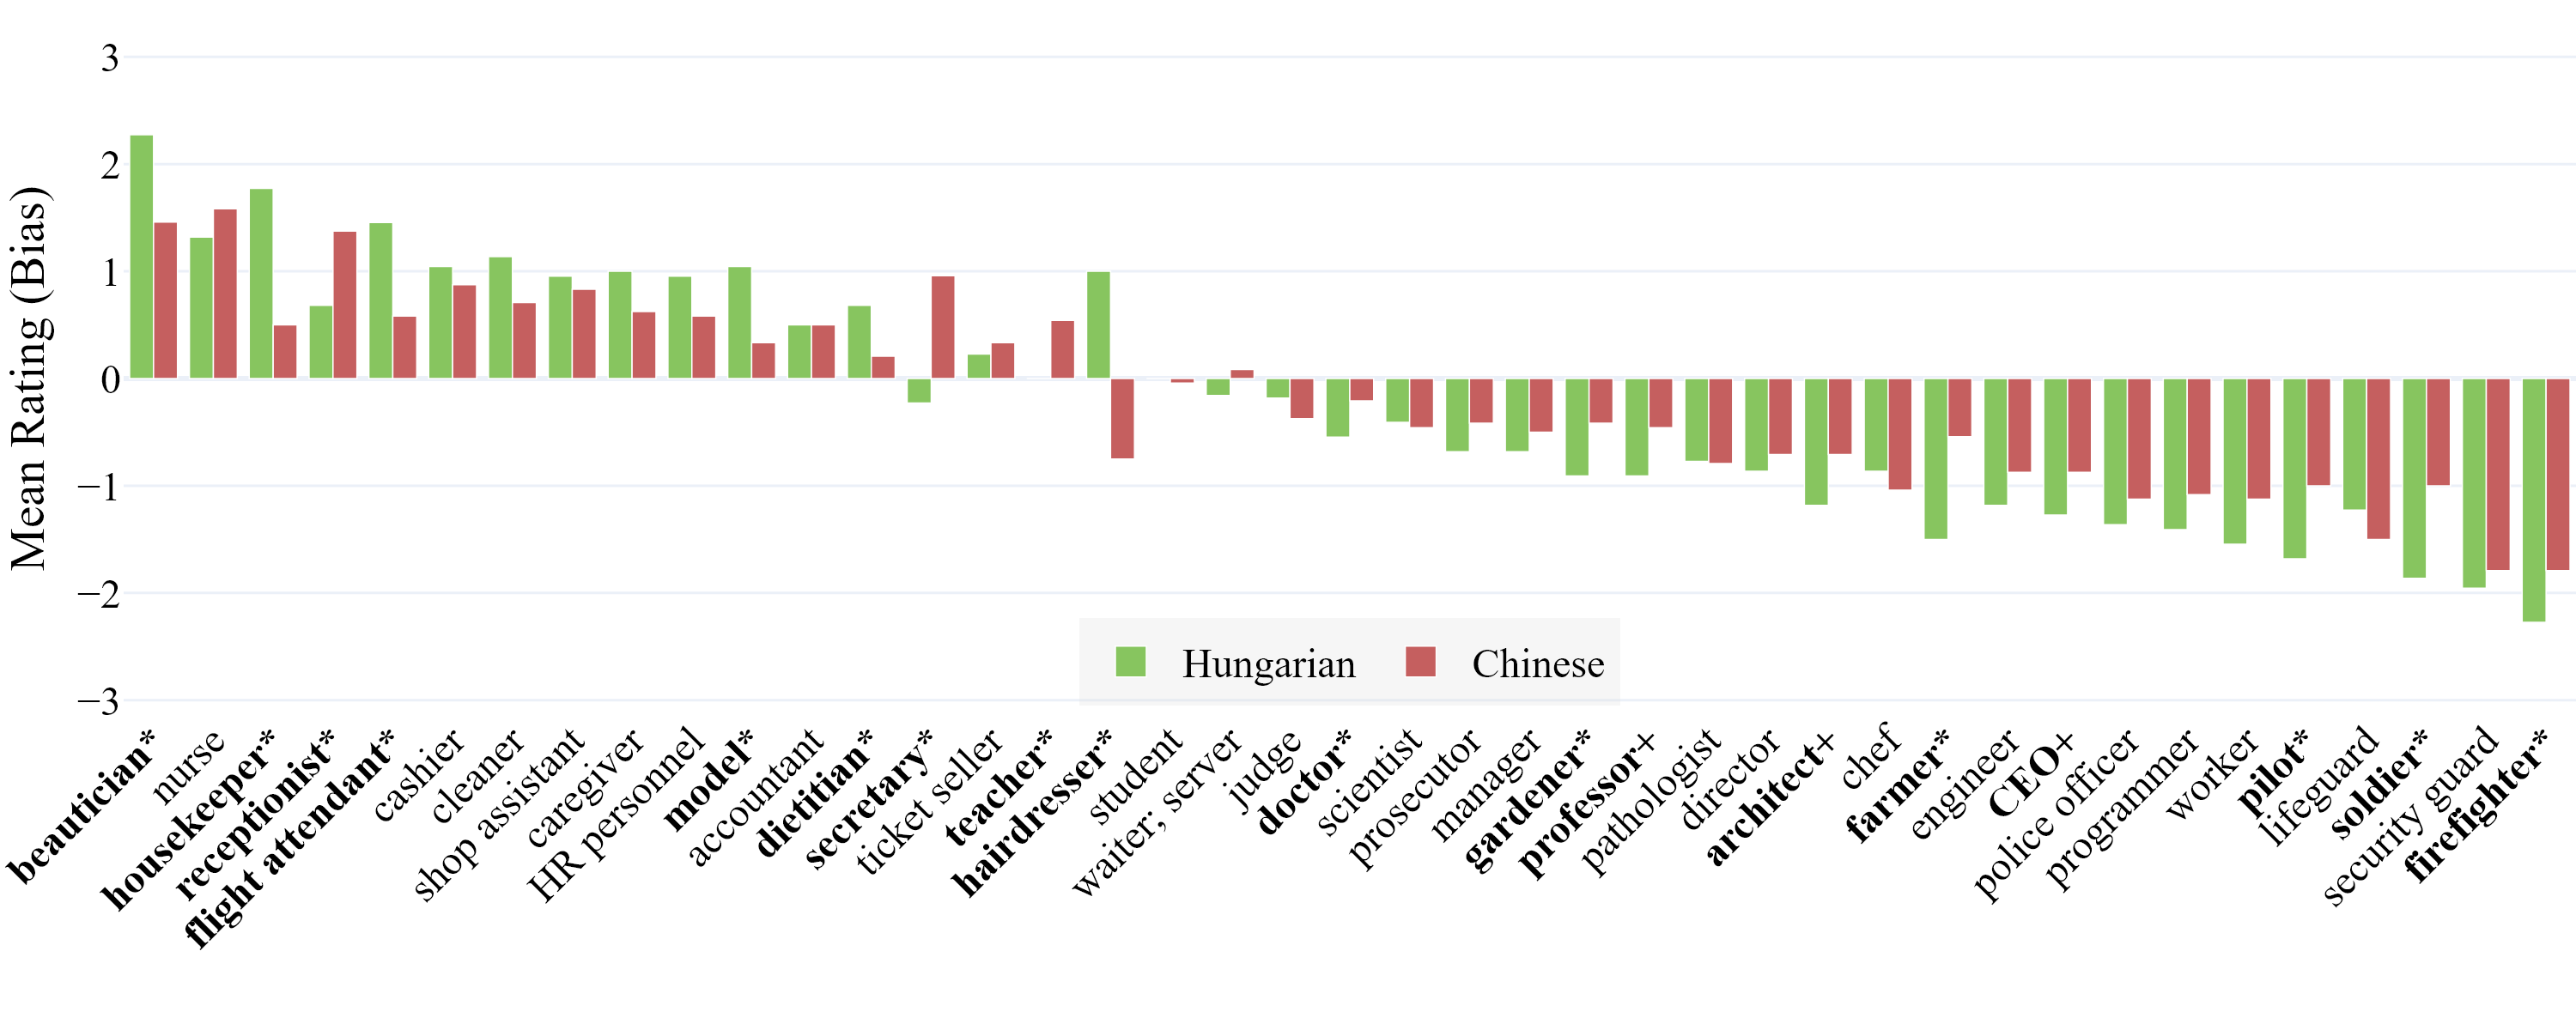
\includegraphics[width=\linewidth]{../occupations_comparison}
%   \caption{Mean ratings of common occupational titles in Hungarian and Chinese (significant*, and marginally significant+ in \textbf{bold}) -- \href{https://anonymous.4open.science/api/repo/occupational-gender-bias/file/occupations_comparison.html?v=8cbb246d}{explore the interactive plot}.}
%   \label{fig:occupations_comparison}
% \end{figure*}

\subsubsection{Intra-language gender differences}

The comparison of the ratings of male vs. female participants indicated significant differences between what people think of a typical \zh{收银员} `cashier' (m: 0.64; w: 1.20), \zh{模特} `model' (m: 0.57; w: 0), \zh{法官} `judge' (m: -0.14; w: 0.70), and \zh{农民} `farmer' (m: -0.79; w: -0.20). Results can be examined in Figure \ref{fig:occupations_zh_gender} of the Appendix.



\subsection{Cross-linguistic comparison}

The 41 overlapping items in the Hungarian and Chinese datasets were tested for significant differences between the ratings in the two languages, using a two-sample \textit{t}-test. See Figure \ref{fig:occupations_comparison} in the Appendix for an overview of the results.

The first noticeable trend is that by and large, the two languages have similar biases for the same occupations. This could suggests that stereotypes are comparable and -- mostly -- consistent across developing societies. Shared items on the extreme ends of the scale include for example `beautician' and `nurse', as well as `firefighter' and `security guard'. Job titles that were neutral/unbiased in both datasets were `student'.

% Table with the top 5 most different ratings with t-stat and p-value

\begin{table}
  \caption{Top 10 most differently rated occupations.}
  \centering
  \begin{tabular}{@{}lccrr@{}}
    \toprule
    \textbf{Occupation} & \textbf{HU} & \textbf{ZH} & \textbf{t-stat} & \textbf{p-value} \\
    \midrule
    hairdresser & 1.00 & -0.75 & 7.31 & 5.74e-09 \\
    housekeeper & 1.77 & 0.50 & 5.03 & 1.00e-05 \\
    flight attend. & 1.45 & 0.46 & 4.59 & 4.22e-05 \\
    farmer & -1.50 & -0.54 & -4.28 & 1.00e-04 \\
    soldier & -1.86 & -1.00 & -4.09 & 1.84e-04 \\
    secretary & -0.23 & 0.96 & -3.98 & 2.66e-04 \\
    beautician & 2.27 & 1.46 & 3.91 & 3.20e-04 \\
    nurse & 0.41 & 1.58 & -3.98 & 4.72e-04 \\
    pilot & -0.12 & 1.23 & -3.45 & 2.00e-03 \\
    model & 1.05 & 0.33 & -3.19 & 3.00e-03 \\
    \bottomrule
  \end{tabular}
  \label{tab:top_different}
  \vspace{-1em}
\end{table}


% Significant differences between Hungarian and Chinese ratings:
% Number of significant differences: 17

% en,hu,zh,mean_hu,mean_zh,mean_difference,t_stat,p_value
% hairdresser,fodrász,理发师,1.0,-0.75,1.75,7.312199986209629,5.736293580683683e-09
% housekeeper,házvezető,家政员,1.7727272727272727,0.5,1.2727272727272727,5.02978833658533,1.0004430519424787e-05
% flight attendant,légiutas-kísérő,乘务员,1.4545454545454546,0.4583333333333333,0.9962121212121213,4.587243492317245,4.2224352777094545e-05
% farmer,földműves,农民,-1.5,-0.5416666666666666,-0.9583333333333334,-4.2781625152861,0.00010022756010441321
% soldier,katona,军人,-1.8636363636363635,-1.0,-0.8636363636363635,-4.086543426949811,0.00018377507992935004
% secretary,titkár,秘书,-0.22727272727272727,0.9583333333333334,-1.1856060606060606,-4.1510978520833826,0.00027213533034765327
% beautician,kozmetikus,美容师,2.272727272727273,1.4583333333333333,0.8143939393939397,3.909668943020703,0.00032029067250357766
% nurse,ápoló,护士,0.4090909090909091,1.5833333333333333,-1.174242424242424,-3.9807363561096287,0.00047213808622151873
% pilot,pilóta,飞行员,-1.6818181818181819,-1.0,-0.6818181818181819,-3.187230903160563,0.0027355909214501583
% model,modell,模特,1.0454545454545454,0.3333333333333333,0.7121212121212122,3.1852388548500588,0.003047683657907094
% receptionist,recepciós,前台,0.6818181818181818,1.375,-0.6931818181818182,-2.611683272919604,0.012377257383991865
% dietitian,dietetikus,营养师,0.6818181818181818,0.20833333333333334,0.4734848484848484,2.5905666645901735,0.013066555155085565
% waiter,pincér,服务员,-0.5,0.08333333333333333,-0.5833333333333334,-2.6311472364382262,0.01372319612133357
% firefighter,tűzoltó,消防员,-2.272727272727273,-1.7916666666666667,-0.4810606060606062,-2.1860799100448998,0.03429839325138778
% teacher,tanár,教师,0.0,0.5416666666666666,-0.5416666666666666,-2.113894473236767,0.041660361580766296
% gardener,kertész,园丁,-0.9090909090909091,-0.4166666666666667,-0.4924242424242424,-2.073820206781514,0.04500389931624605
% doctor,orvos,医生,-0.5454545454545454,-0.20833333333333334,-0.33712121212121204,-2.0543396200526125,0.04627231293429205


Moreover, we found 17 occupations that were rated statistically differently in the two languages. Moving in descending order from the job titles shoving the starkest contrast, the top 10 are presented in Table \ref{tab:top_different}.

The most obvious dissimilarity was found the word for `hairdresser' (\textit{fodrász} vs. \zh{理发师}), which showed a strong female bias in Hungarian (1.00) but a definite male bias in Chinese (-0.75). We believe that this is a neat example for a societal difference, and the only one with serious opposing polarity; in Hungary hairdressers are perceived to be predominantly female, while in China the profession is perceived to be more male-dominated -- although the gap is closing.\footnote{It is not difficult to find evidence for the latter from the press, even in English-language media: \href{https://www.chinadailyhk.com/hk/article/603100\#Women-raise-the-hairdressing-bar--2025-01-23}{https://www.chinadailyhk.com/hk/article/603100\#Women-raise-the-hairdressing-bar--2025-01-23}}

% \citep{nan_2025_women}

% \hl{New from Wenhui from here...}

The gender stereotype linked to `housekeeper' is predominantly female in both cultures; however, the extent of this bias varies considerably (Chinese: 0.5 vs. Hungarian: 1.77). In the results of Chinese participants, it is pertinent to compare the terms \zh{家政员} \textit{jiāzhèngyuán} meaning `housekeeper' and \zh{保姆} \textit{baómǔ} meaning `nanny', which are analogous in meaning yet vary in register. While the term `housekeeper' (0.5) demonstrates less gender bias than the colloquial term `nanny' (1.63), it remains categorised as a female-dominated profession due to the traditional female-associated traits of household tasks and emotional management suggested by the central term \zh{家政} \textit{jiāzhèng} `housekeeping'. This domain-specific scoring disparity indicates that although the formal and informal characteristics of occupational terminology mitigate gender stereotypes, societal gender stereotypes regarding occupations may be intricately linked to the semantic implications of language. Particular terminology related to domestic or emotional labour is more prone to evoke conventional female gender bias perceptions, thus reinforcing the gendered classification of professions.

The job title `secretary' also elicits significantly different gender stereotypes among Hungarian and Chinese participants. Hungarian participants perceive \textit{titkár} as a marginally male-dominated profession (-0.23), whereas Chinese participants perceive it a predominantly female occupation (0.96). This discrepancy may arise from the interaction of lexical attributes and a (post-)socialist cultural context. In Hungarian, \textit{titkár} denotes both senior political officials and regular administrative employees, however the female-marked form \textit{titkárnő} can only refer to an administrative employee. Conversely, the Chinese Occupational Classification Dictionary delineates a \zh{秘书} \textit{mìshū} `secretary' as an office service employee involved in clerical and meeting-related responsibilities. This definition may delay the manifestation of societal perception and gender expectations, yet it largely corresponds with public expectations of the secretary profession. The semantic scope and societal expectations of identical occupational titles in Hungarian and Chinese illustrate how cultural background influences gender bias in vocabulary.

% (Occupational Code: 3-01-02-02)

The disparities in gender perception between `farmer' and `worker' are particularly significant. Data from Chinese participants indicates that `farmer' (-0.54) demonstrates a comparatively weaker male orientation than `worker' (-1.13), whereas in Hungarian, the two are nearly identical (farmer: -1.50 vs. worker: -1.55). This discrepancy can be attributed to China’s societal and economic development trajectory. Throughout the era of collective farming in China (1950s–-1970s), the work-point accounting system and production brigades promoted women's involvement in agricultural labour, while slogans such as ``Women hold up half the sky'' (\zh{妇女能顶半边天}) enhanced the visibility of women in this sector \citep{jacka_1997_agriculture,jacka_1997_domestic}. Despite the Household Contract Responsibility System established in the 1980s reinforcing the dominance of male household heads and consequently marginalising women's land rights \citep{zhu_2009_gender}, the significance of women in agricultural production has progressively become apparent [data is needed here to show the proportion of women in the Chinese agriculture industry]. During this period, township enterprises and factories employed female labour; however, they confined women to light industrial positions through technical qualification prerequisites \citep{liu_2007_gender}. This led to a gendered labour division in which women in industry participated in unskilled roles, while men retained technical monopolies \citep{bossen_2002_chinese}. This historical process has resulted in the ongoing divergence of gender perceptions between the agricultural and industrial sectors. Despite contemporary ideals of occupational gender equality, gender stereotypes in lower-tier professions continue to demonstrate significant historical persistence.

% \hl{...to here}



\subsection{Discussion}\label{sec:discussion}

We asked a question on how much gender stereotypes would manifest in Hungarian and Chinese occupational titles -- words without grammatical gender markings -- and found that societal gender stereotypes mostly pierce through the words. We have found a few significant distinctions between the ratings of men and women, and noteworthy differences and similarities in the way certain professions are perceived in Hungarian and Chinese contexts. The key takeaway is that the absence of grammatical gender does not prevent strong gender stereotypes from being encoded in work-related lexicon, and that bias likely roots from cultural norms, social knowledge, and and extralinguistic context, which are then reflected in word associations. This in itself is not surprising and it is consistent with previous studies on similar languages, such as Estonian \citet{kaukonen_2025_gender}. Cross-culturally, the findings suggest that in general the underlying gender biases are often a shared phenomenon, but specific terms may differ. According to participants, hairdressers are predominantly women in Hungary, but mostly men in China, which is a strong example of cultural/social specificity.

\subsubsection{Gender bias by language}

An interesting finding is that Hungarian raters tended to rate occupations with a stronger bias than Chinese speakers. Out of 41 shared occupations, 30 were rated with a significant bias in Hungarian, while only 10 were rated with a higher bias in Chinese (excluding the 1 item with equal value). This is a threefold difference (cf. Fig. \ref{fig:bias_counts}), and warrants further exploration to fully explain. We could consider the linguistic, social, and historic similarities with Estonian -- another ungendered Uralic language with relatively high biases when compared to Russian \citep{kaukonen_2025_gender} -- but the variables are simply too many to consider. 

% \begin{figure}[!ht]
%   \centering
%   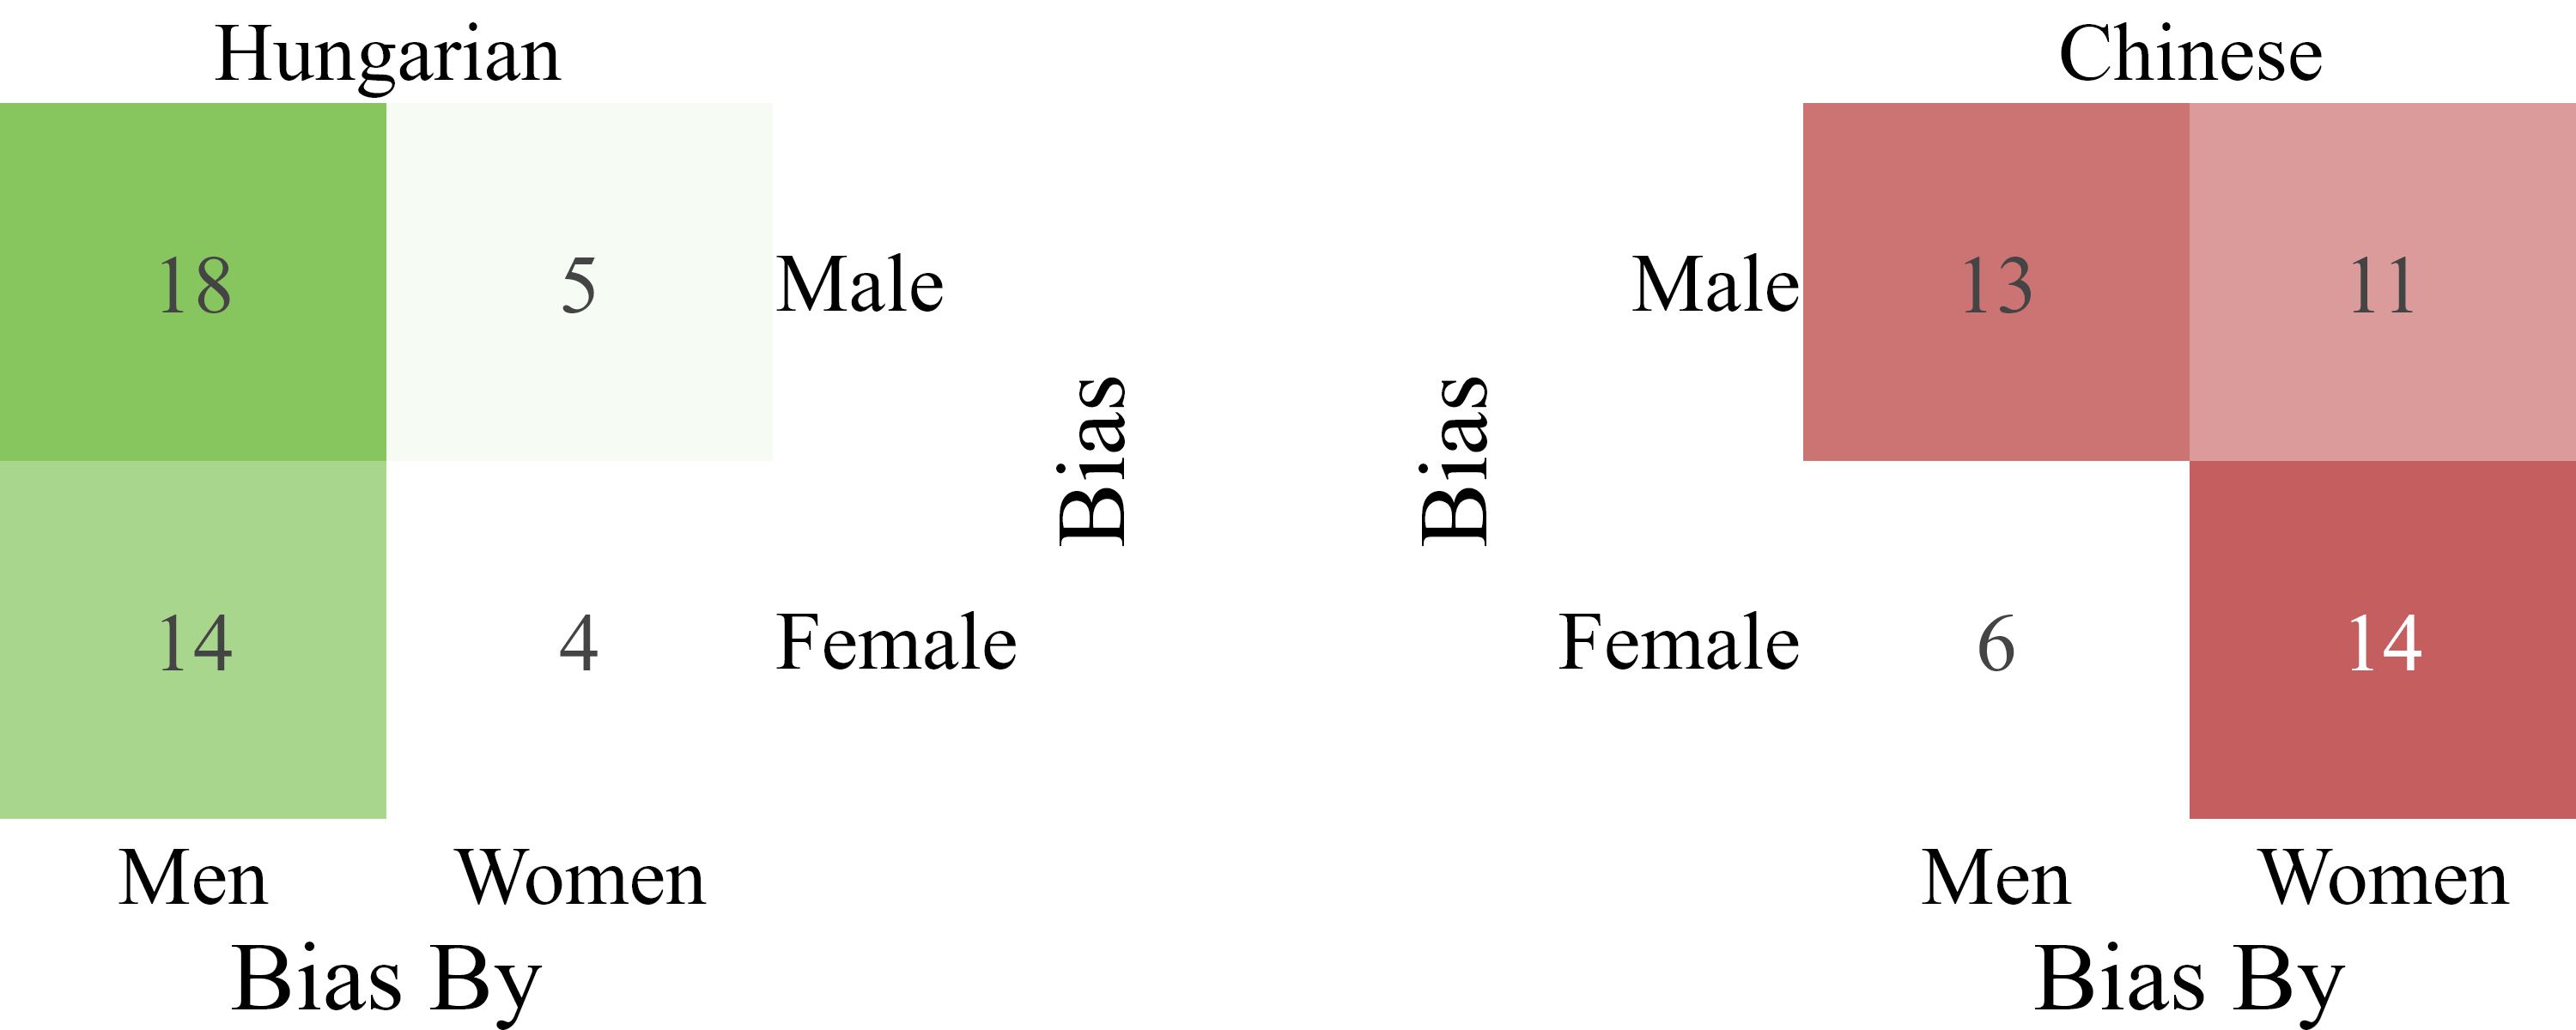
\includegraphics[width=\linewidth]{../confusion_matrices}
%   \caption{Confusion matrix of the Hungarian and Chinese ratings, showing the differences in the ratings of male and female participants.}  
%   \label{fig:confusion_matrices}
% \end{figure}

\subsubsection{Gender bias by language users' gender}

Another interesting divergence arose when comparing the two datasets and the differences between the ratings by gender. While in Hungarian, biases -- both male and female -- were stronger in the ratings of men, in Chinese, women rated with a stronger bias on average; especially regarding female biases. The reason for this could be due to personal experiences and social norms in the respective cultures, and the various ways in which gender is perceived in each society. We plotted the discrepancies as confusion matrices in Figure \ref{fig:confusion_matrices}.

% \begin{figure*}[!ht]
%   \centering
%   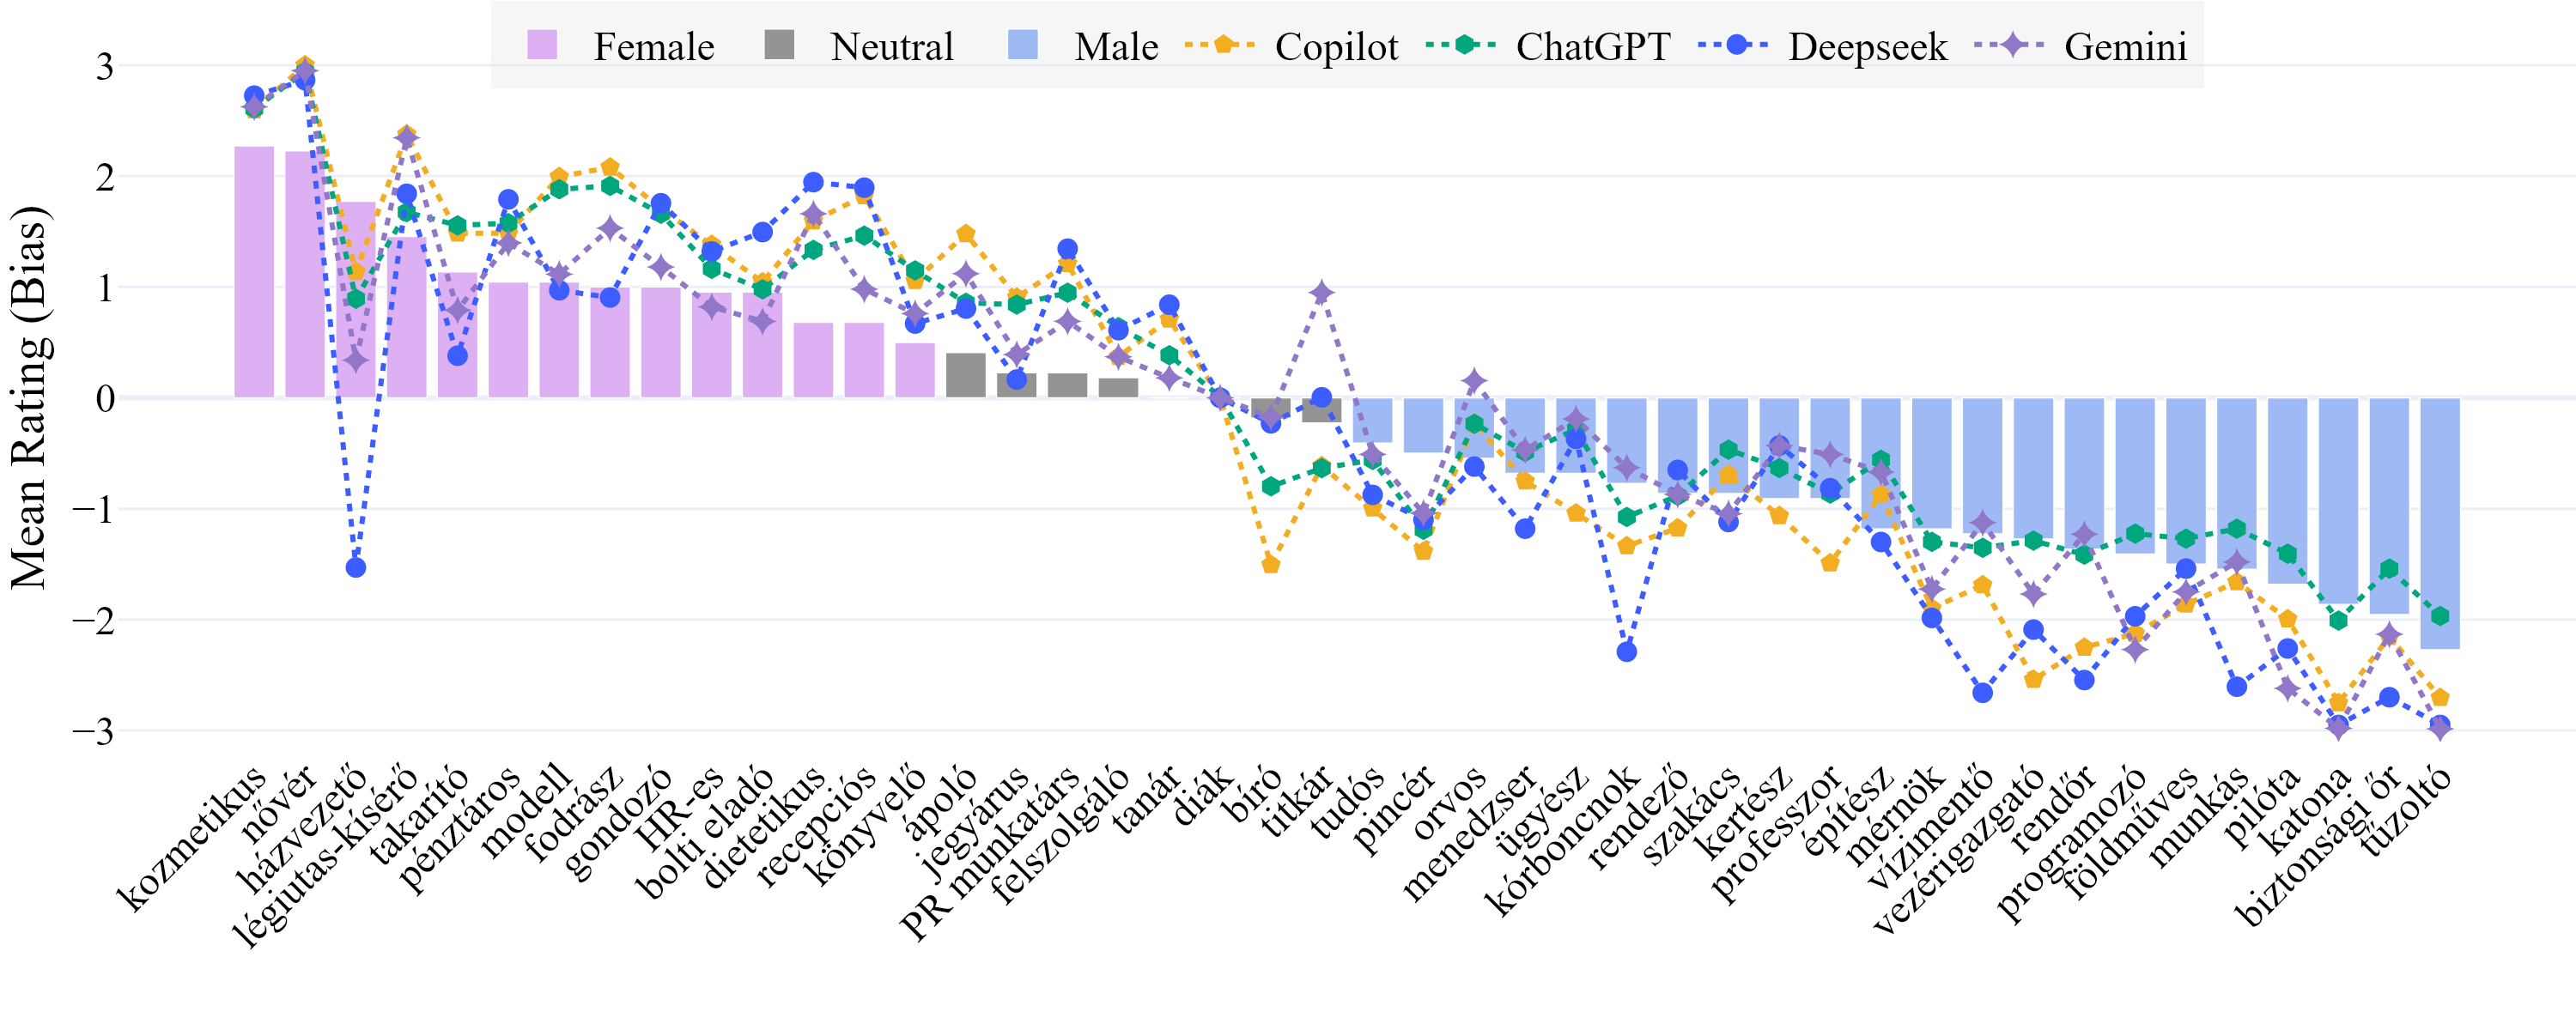
\includegraphics[width=\linewidth]{../occupations_hu_with_ai}
%   \caption{AI ratings for Hungarian occupations \href{https://anonymous.4open.science/api/repo/occupational-gender-bias/file/occupations_hu_with_ai.html?v=87b2469e}{--- explore the interactive plot}.}
%   \label{fig:occupations_hu_with_ai}
% \end{figure*}

% \begin{figure*}[tbp]
%   \centering
%   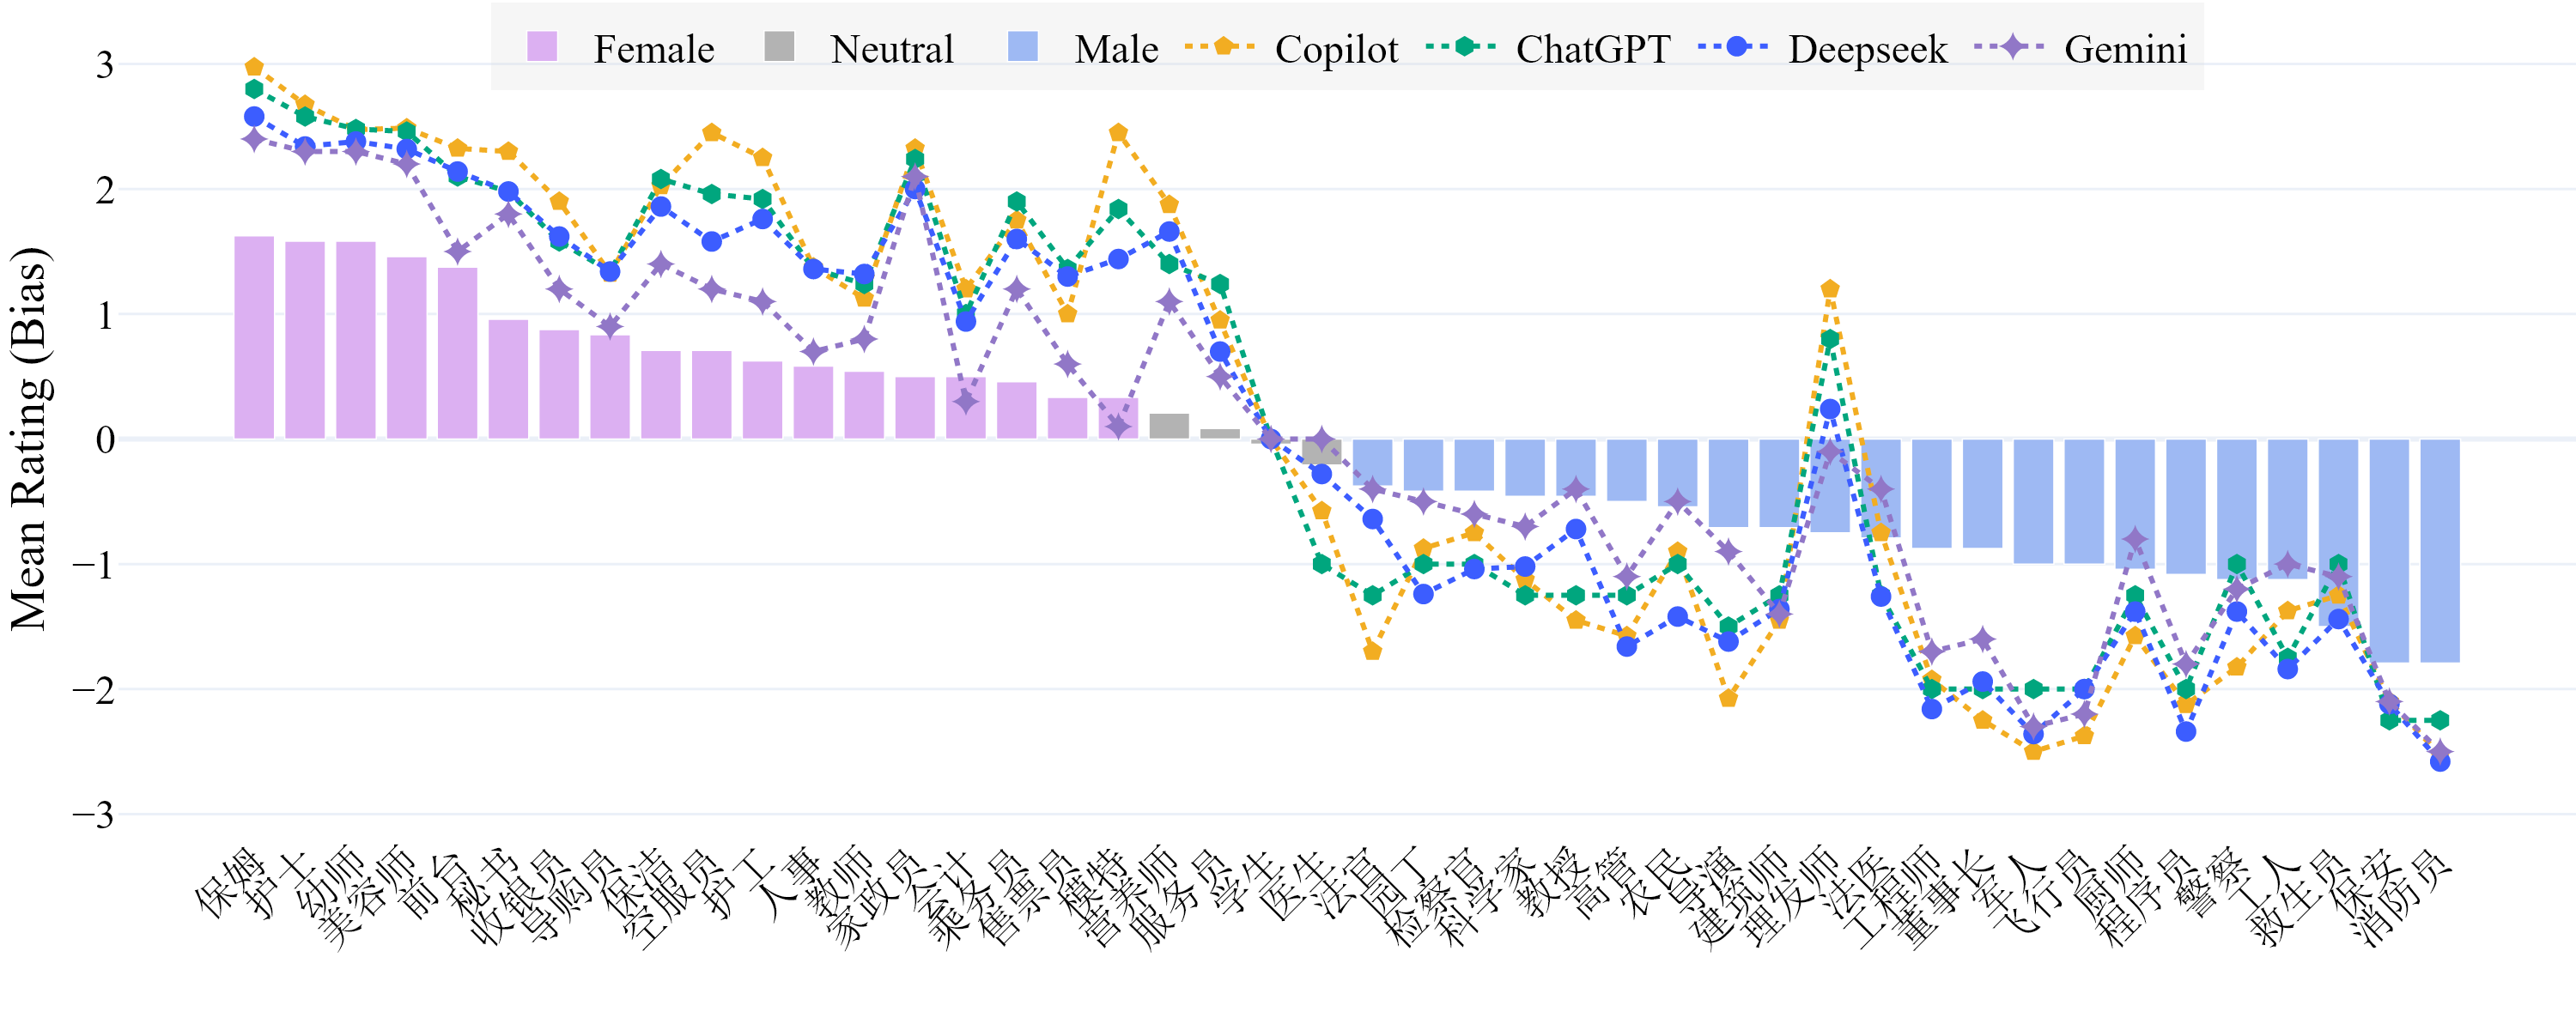
\includegraphics[width=\linewidth]{../occupations_zh_with_ai}
%   \caption{AI ratings for Chinese occupations \href{https://anonymous.4open.science/api/repo/occupational-gender-bias/file/occupations_zh_with_ai.html?v=00fce30d}{--- explore the interactive plot}.}
%   \label{fig:occupations_zh_with_ai}
% \end{figure*}

Noticing and acknowledging these gender biases have real-world implications, take for instance professionals working in career counseling, or job advertisements using language better suited for equal opportunities. Modern AI systems learn from existing societal biases, and they may inadvertently amplify these issues, making it essential to address it proactively.

% giving more nuanced advice

\section{Comparing human ratings with AI-generated ratings}
\label{sec:ai_comparison}

Finally, we were curious how the human ratings compare to the ratings of LLMs used by popular AI agents and chatbots, so we repeated the same experiment using artificial intelligence instead of human raters. From Mistral's Le Chat, Copilot, ChatGPT, Deepseek, and Gemini the mean AI ratings and standard deviations were then superimposed on the human raters' plots to allow for a convenient comparison, as shown in Figures \ref{fig:occupations_hu_with_ai} and \ref{fig:occupations_zh_with_ai}.

The rationale behind this was to simulate how the general public and non-experts would turn to AI to do the job of -- sometimes expensive -- human raters, so we purposefully avoided any pre-training or fine-tuning that requires a degree of technical know-how, and used the best available versions that were available in this timeframe on a free tier, in quota, on their respective web interfaces. We performed a correlation test using Pearson's \textit{R} to compare the human and AI ratings to find out which models did the best compared to humans, and we found very strong positive correlations between the sets of ratings in both languages, see Table \ref{tab:correlation}.

% Put a table here with two subtables, Hungarian on the left, Chinese on the right

\begin{table}
  \caption{Correlation between human and AI ratings for occupational titles in Hungarian and Chinese, sorted by the correlation coefficient.}
  \centering
  \begin{tabular}{@{}l|l|c|c@{}}
    \textbf{\#} & \textbf{Hungarian} & \textbf{R} & \textbf{p\_value} \\
    \hline
    1 & LeChat & 0.9634 & < 0.01 \\
    2 & Gemini & 0.9529 & < 0.01 \\
    3 & ChatGPT & 0.9525 & < 0.01 \\
    4 & Copilot & 0.9255 & < 0.01 \\
    5 & DeepSeek & 0.8768 & < 0.01 \\

    \textbf{\#} & \textbf{Chinese} & \textbf{R} & \textbf{p\_value} \\
    \hline
    1 & DeepSeek & 0.9504 & < 0.01 \\
    2 & Gemini & 0.9452 & < 0.01 \\
    3 & LeChat & 0.9313 & < 0.01 \\
    4 & ChatGPT & 0.9235 & < 0.01 \\
    5 & Copilot & 0.9156 & < 0.01 \\
  \end{tabular}
  \label{tab:correlation}
\vspace{-1em}
\end{table}

The results show that the LLMs in these AI agents are performing really well, showing converging trends. For Hungarian, the closest results showing the highest correlation of 0.9634 were achieved by using Mistral AI's Le Chat, the only European model in our experiment. In turn, the best results for Chinese were obtained with DeepSeek, which achieved a correlation of 0.9504. 

However, it is to be emphasised that these practices can be highly problematic, as the biases encoded in the LLMs are even stronger than those of the human raters, and publishing studies that use LLMs instead of participants can reinforce gender biases. We think that the results perfectly illustrate both the pros and cons (or dangers?) of using AI agents instead of human raters, especially as they can perpetuate social biases.



\section{Conclusion}

In conclusion, our study provided experimental evidence for the existence of deep-seated occupational gender biases on the lexical level, and that linguistically ungendered occupational nouns in Hungarian and Chinese are nevertheless loaded with people's social gender stereotypes relating to these occupations. We have also demonstrated that the biases are -- mostly -- comparable across two distant societies, and maybe presumably everywhere in the developed, globalized world. Lastly, we have made our datasets -- both human and AI -- publicly available to facilitate future comparisons.

\subsection{Limitations and future directions}

An obvious limitation of this study is that the specific set of jobs chosen does not fully represent the diversity of the many career paths people pursue. Future research should expand the list of occupations and also include more languages to gain a more comprehensive understanding of occupational gender biases. 

% Furthermore, it would be meaningful to compare actual workforce statistics on gender distribution per profession in the two countries to see how much the ratings reflect reality.



% Bibliography entries for the entire Anthology, followed by custom entries
%\bibliography{anthology,custom}
% Custom bibliography entries only
\bibliography{custom}

\appendix

\section{Appendix}
\label{sec:appendix}

\subsection{Hungarian items}\label{sec:hungarian_items}

\textit{modell}, \textit{katona} `soldier', \textit{kórboncnok} `pathologist', \textit{vezérigazgató} `CEO', \textit{menedzser}, `manager' \textit{nővér}, `nurse' \textit{szakács} `chef', \textit{felszolgáló} `server', \textit{könyvelő} `accountant', \textit{professzor} `professor', \textit{építész} `architect', \textit{tudós} `scientist', \textit{ápoló} `nurse', \textit{pénztáros} `cashier', \textit{bíró} `judge', \textit{munkás} `worker', \textit{vízimentő} `lifeguard', \textit{jegyárus} `ticket seller', \textit{tűzoltó} `firefighter', \textit{mérnök} `engineer', \textit{rendező} `director', \textit{takarító} `cleaner', \textit{HR-es} `HR specialist', \textit{házvezető} `housekeeper', \textit{légiutas-kísérő} `flight attendant', \textit{pincér} `waiter', \textit{orvos} `doctor', \textit{fodrász} `hairdresser', \textit{földműves} `farmer', \textit{gondozó} `caregiver', \textit{bolti eladó} `shop assistant', \textit{kertész} `gardener', \textit{titkár} `secretary', \textit{PR munkatárs} `PR officer', \textit{dietetikus} `dietitian', \textit{tanár} `teacher', \textit{rendőr} `police officer', \textit{pilóta} `pilot', \textit{recepciós} `receptionist', \textit{biztonsági őr} `security guard', \textit{ügyész} `prosecutor', \textit{kozmetikus} `beautician', \textit{programozó} `programmer', \textit{diák} `student'.

\subsection{Chinese items}\label{sec:chinese_items}

\zh{警察} `police', \zh{秘书} `secretary', \zh{教授} `professor', \zh{护士} `nurse', \zh{高管} `manager', \zh{教师} `teacher', \zh{前台} `receptionist', \zh{工人} `worker', \zh{幼师} `kindergarten teacher', \zh{模特} `model', \zh{护工} `caregiver', \zh{保姆} `nanny', \zh{会计} `accountant', \zh{工程师} `engineer', \zh{保洁} `cleaner', \zh{法官} `judge', \zh{导购员} `shop assistant', \zh{美容师} `beautician', \zh{服务员} `waiter', \zh{乘务员} `flight attendant'\footnote{Also the attendant/crew on high-speed trains.}, \zh{理发师} `hairdresser', \zh{空服员} `flight attendant'\footnote{Less frequent word; only on airplane.}, \zh{售票员} `ticket seller', \zh{厨师} `chef', \zh{营养师} `nutritionist', \zh{家政员} `housekeeper', \zh{收银员} `cashier', \zh{医生} `doctor', \zh{法医} `pathologist', \zh{程序员} `programmer', \zh{保安} `security guard', \zh{导演} `director', \zh{军人} `soldier', \zh{董事长} `CEO', \zh{农民} `farmer', \zh{学生} `student', \zh{园丁} `gardener', \zh{飞行员} `pilot', \zh{人事} `HR personnel', \zh{消防员} `firefighter', \zh{科学家} `scientist', \zh{检察官} `prosecutor', \zh{救生员} `lifeguard', \zh{建筑师} `architect'.


\begin{figure*}[!ht]
  \centering
  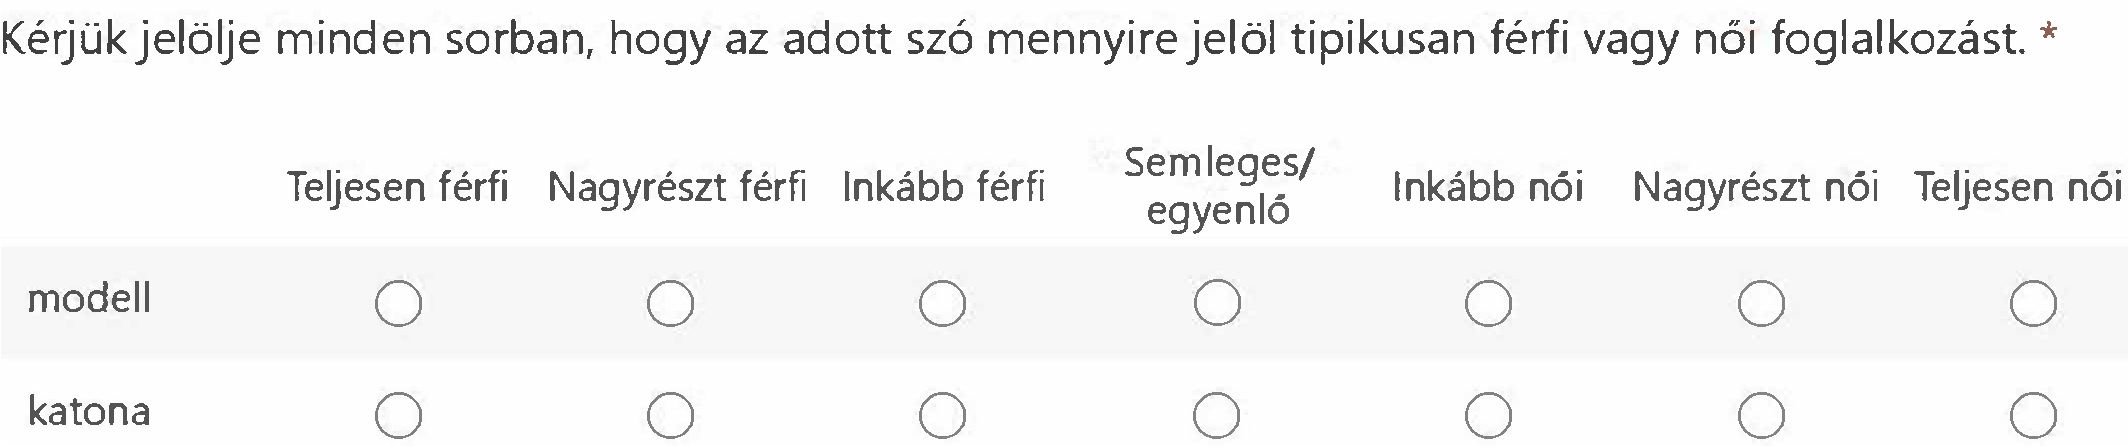
\includegraphics[width=\linewidth]{../survey_hu}
  \caption{A sample of the the Hungarian survey layout.}
  \label{fig:survey_hu}
\end{figure*}

\begin{figure*}[!ht]
  \centering
  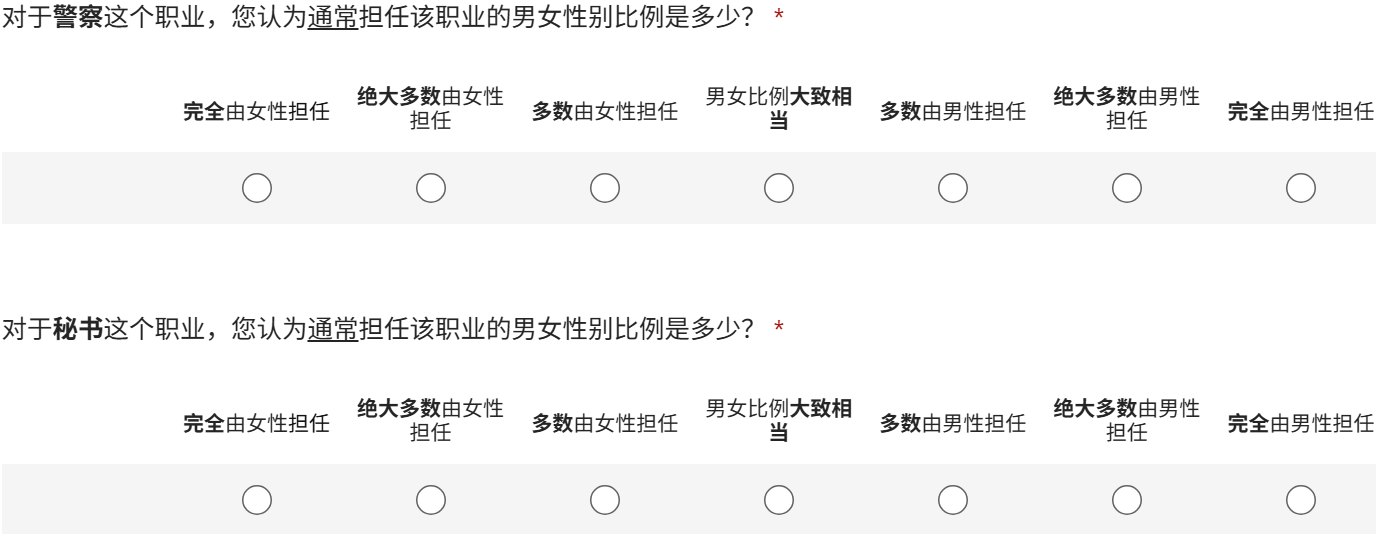
\includegraphics[width=\linewidth]{../survey_zh}
  \caption{A sample of the the Chinese survey layout.}
  \label{fig:survey_zh}
\end{figure*}




\begin{figure}[!ht]
  \centering
  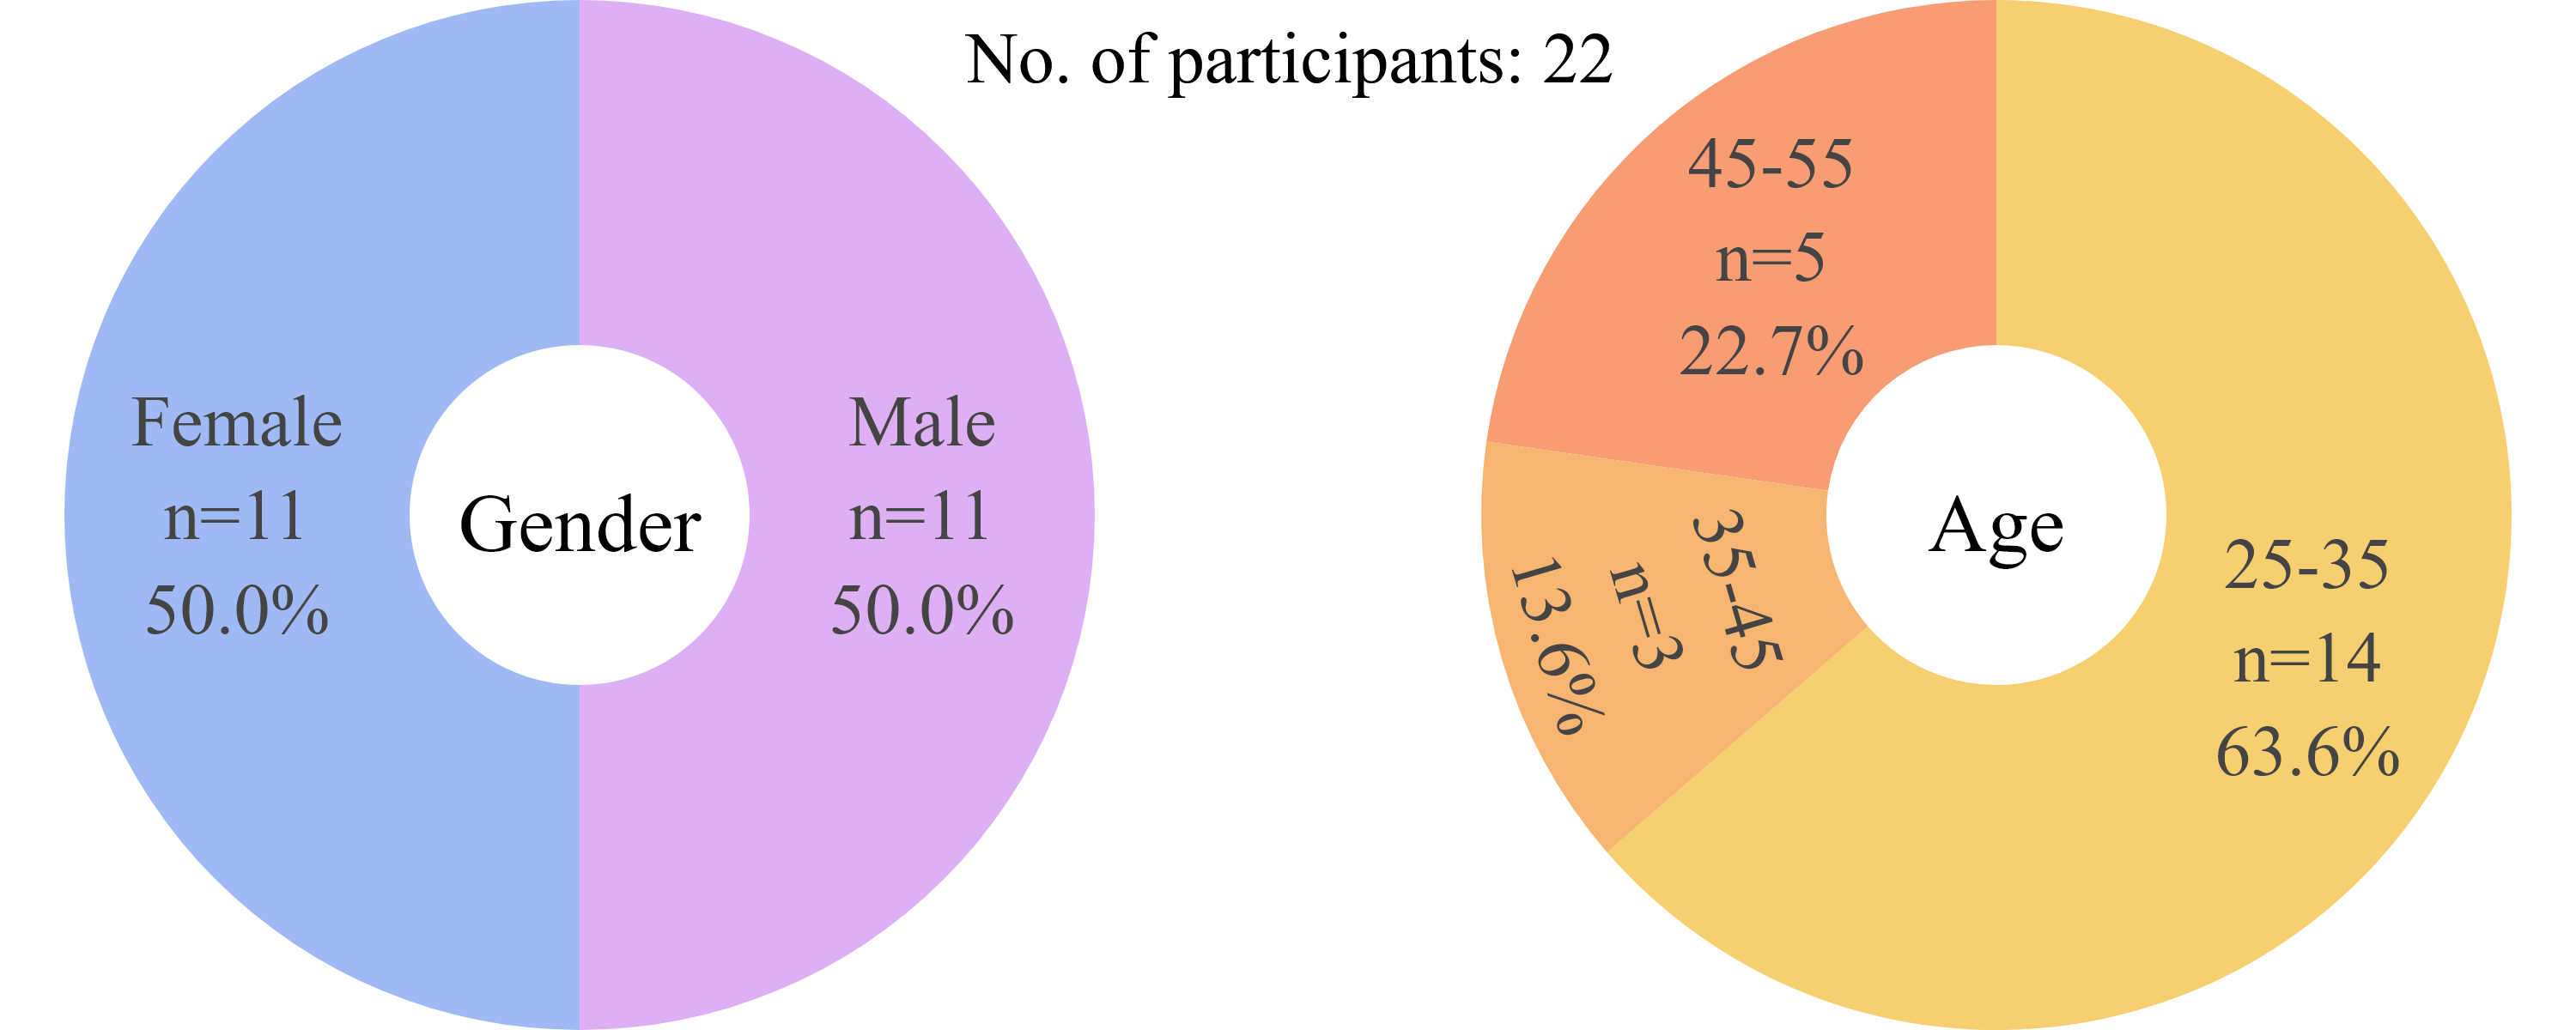
\includegraphics[width=\linewidth]{../demographics_hu}
  \caption{Demographics of the Hungarian participants.}
  \label{fig:demographics_hu}
\end{figure}

\begin{figure}[!ht]
  \centering
  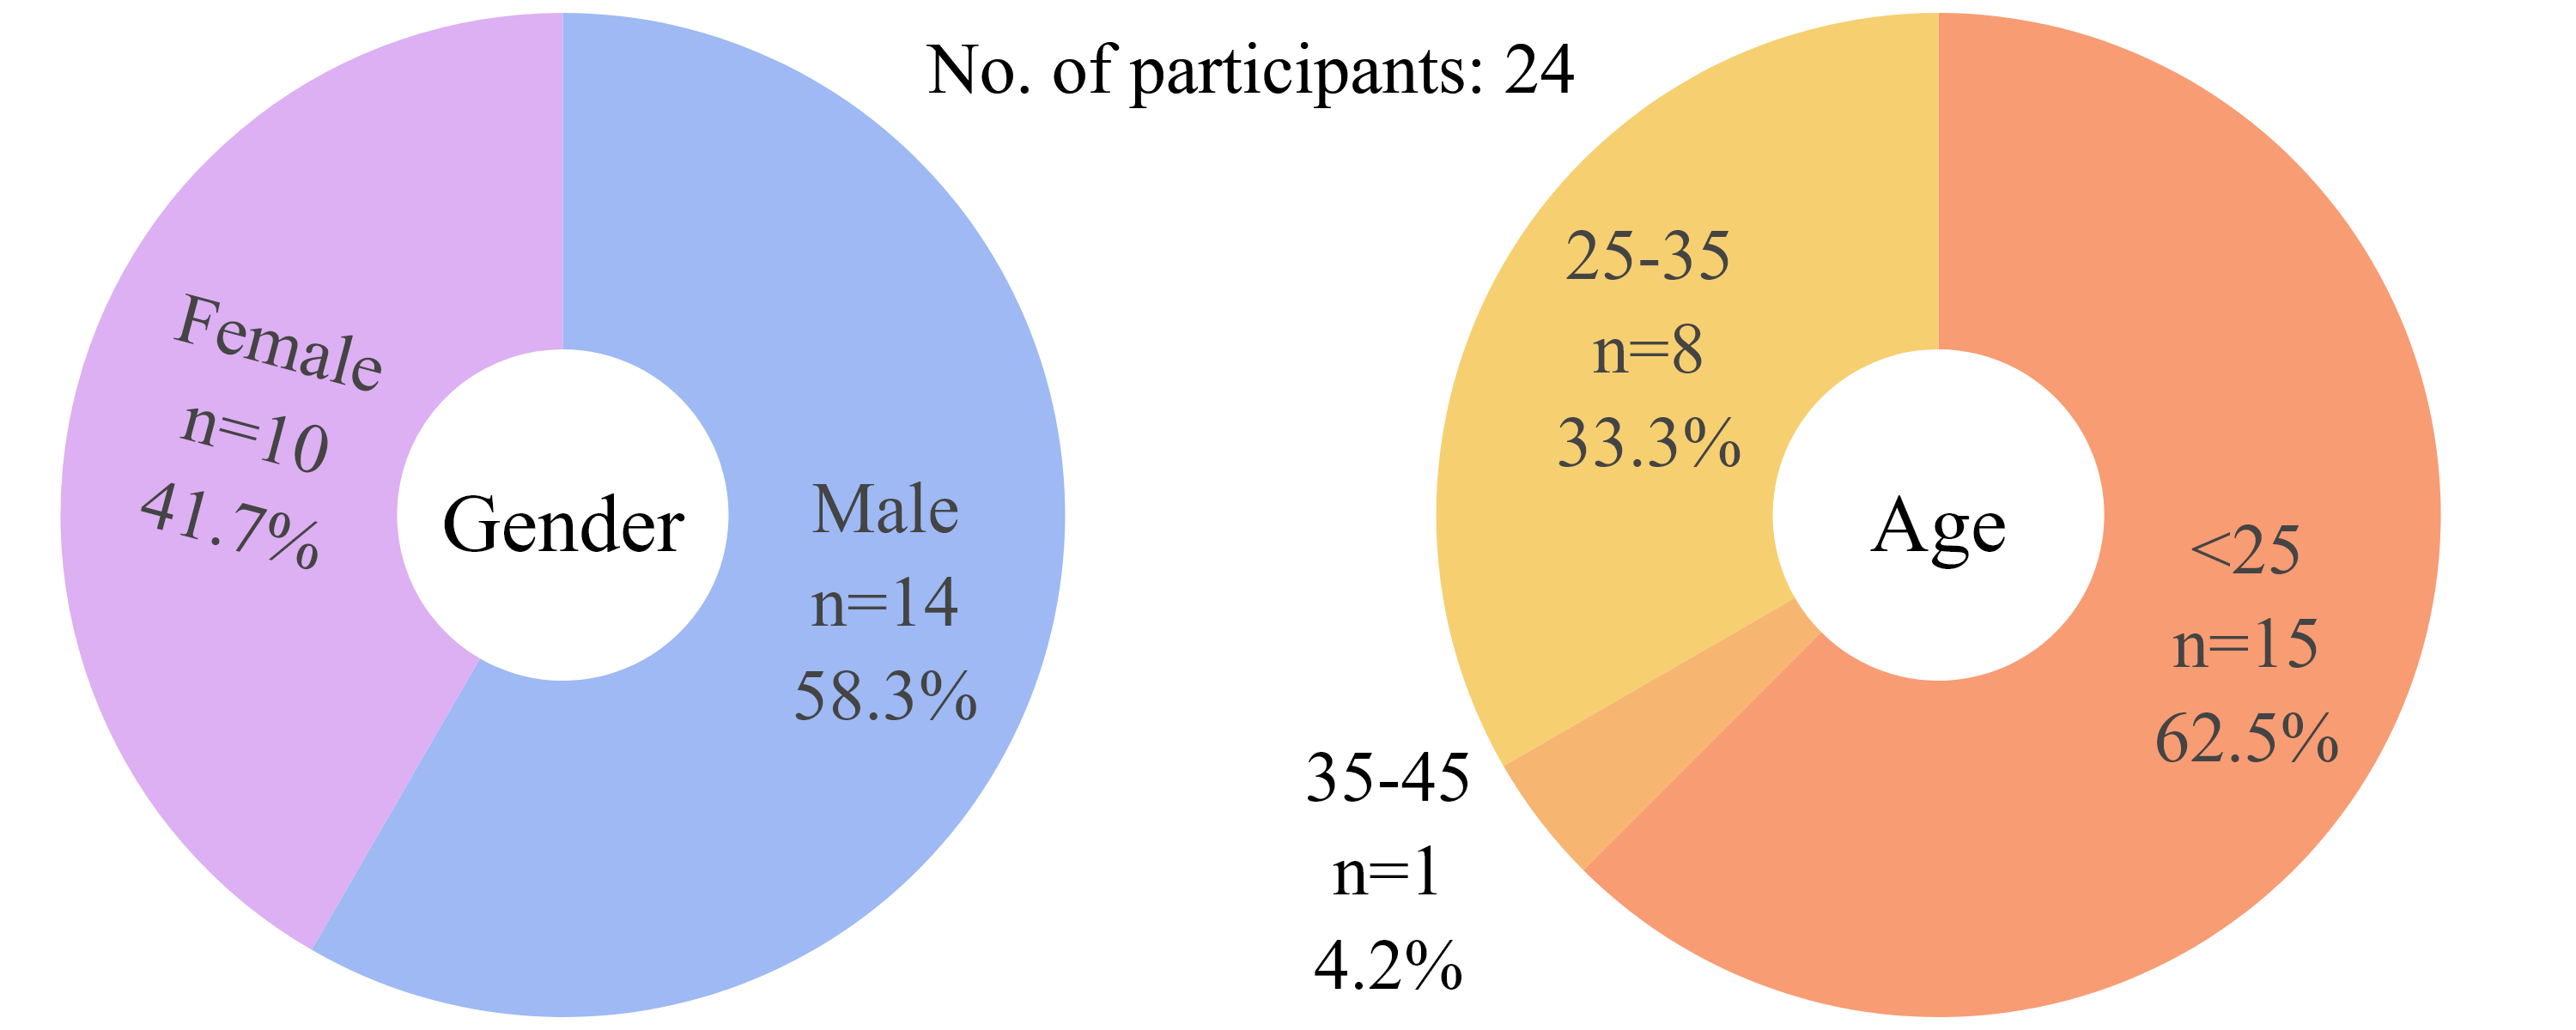
\includegraphics[width=\linewidth]{../demographics_zh}
  \caption{Demographics of the Chinese participants.}
  \label{fig:demographics_zh}
\end{figure}

\bigskip

\begin{figure}[b]
  \centering
  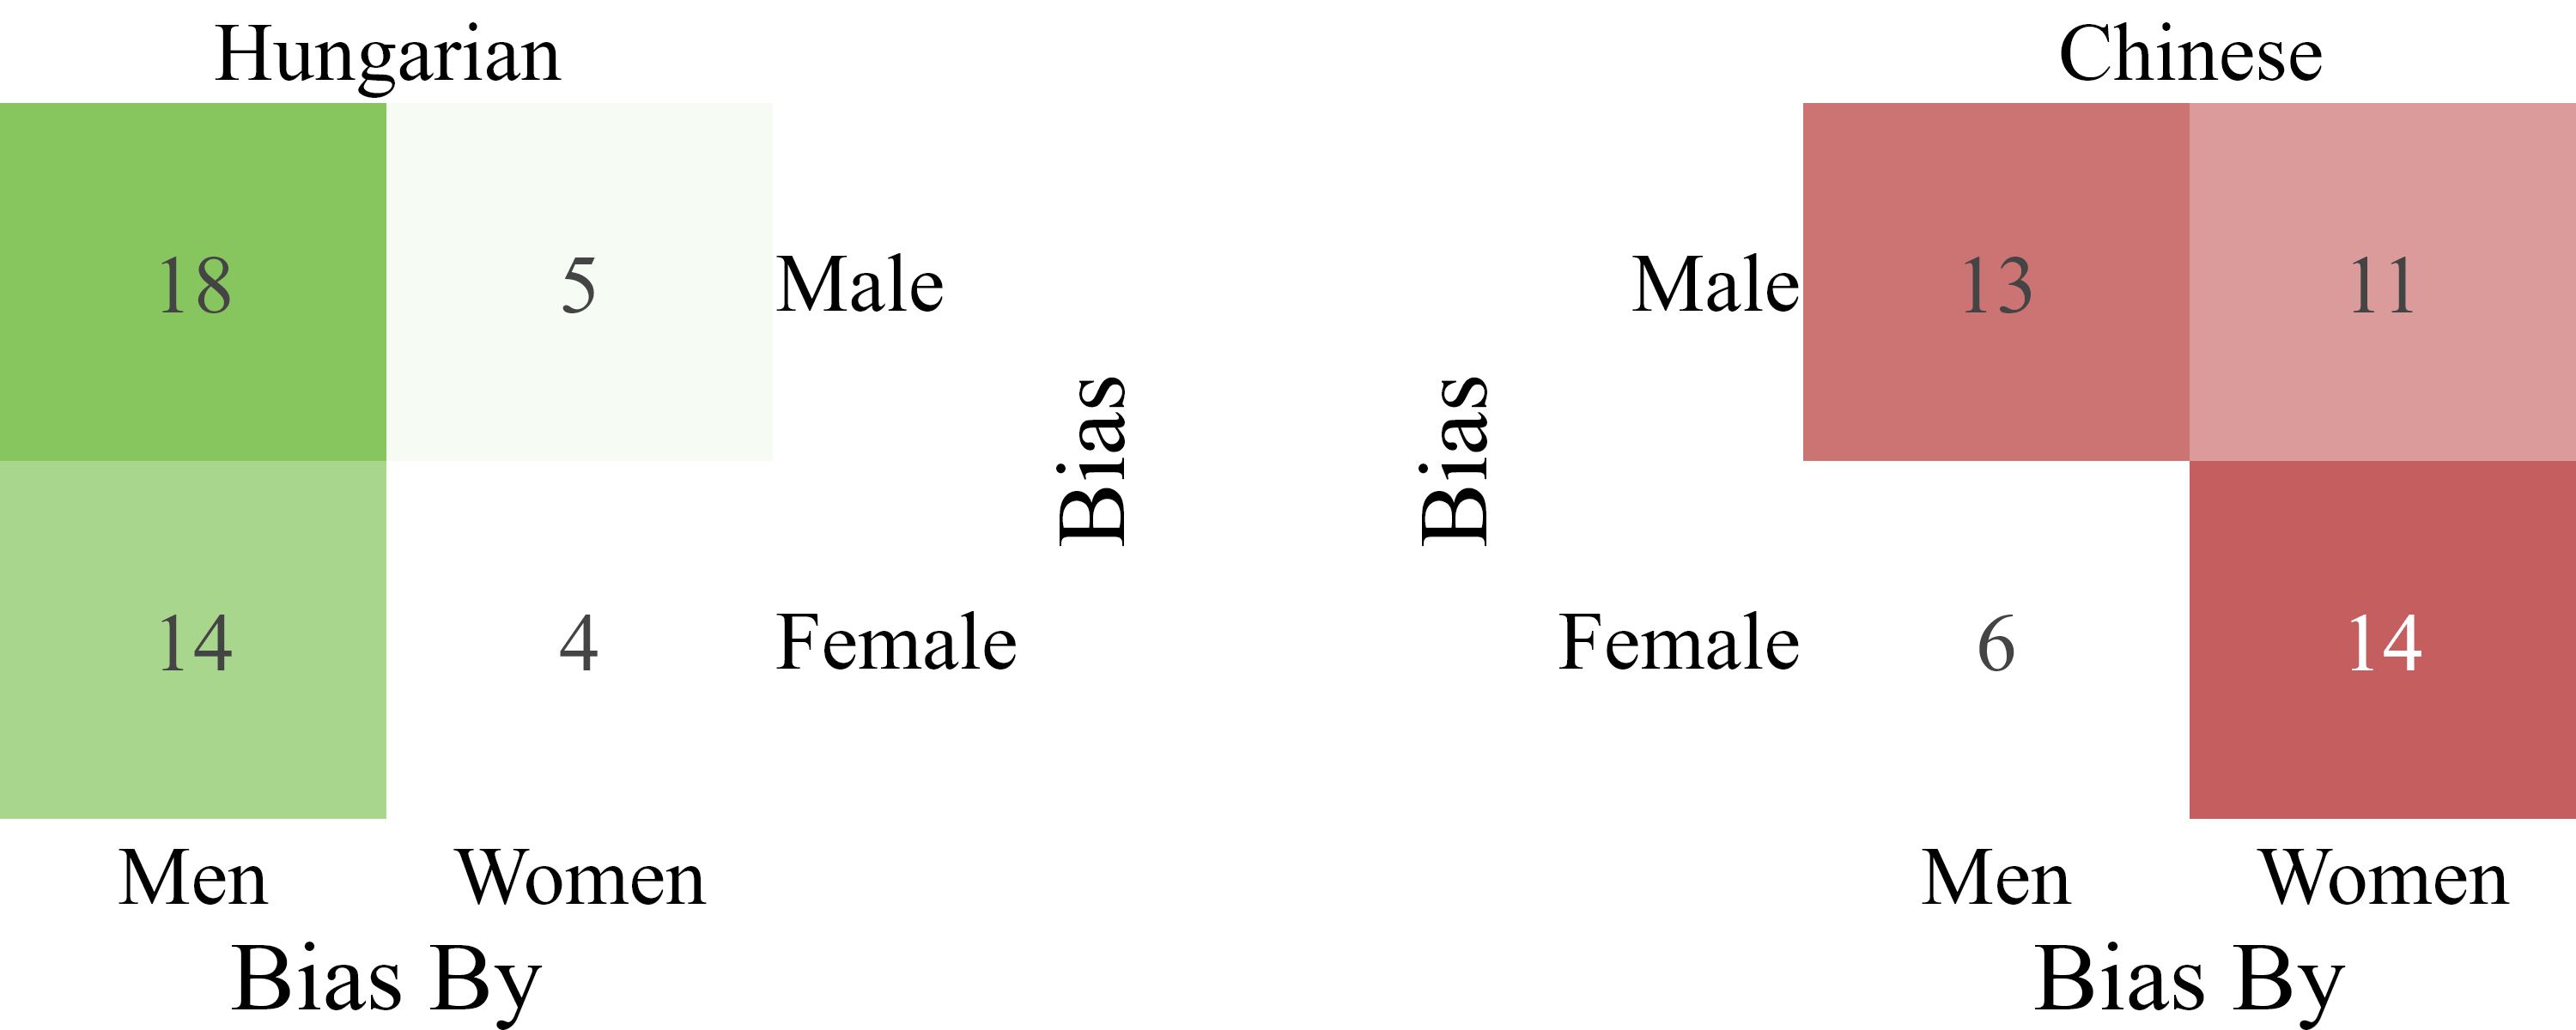
\includegraphics[width=\linewidth]{../confusion_matrices}
  \caption{Confusion matrix of the Hungarian and Chinese ratings, showing the differences in the ratings of male and female participants.}  
  \label{fig:confusion_matrices}
\end{figure}

\begin{figure}[b]
  \centering
  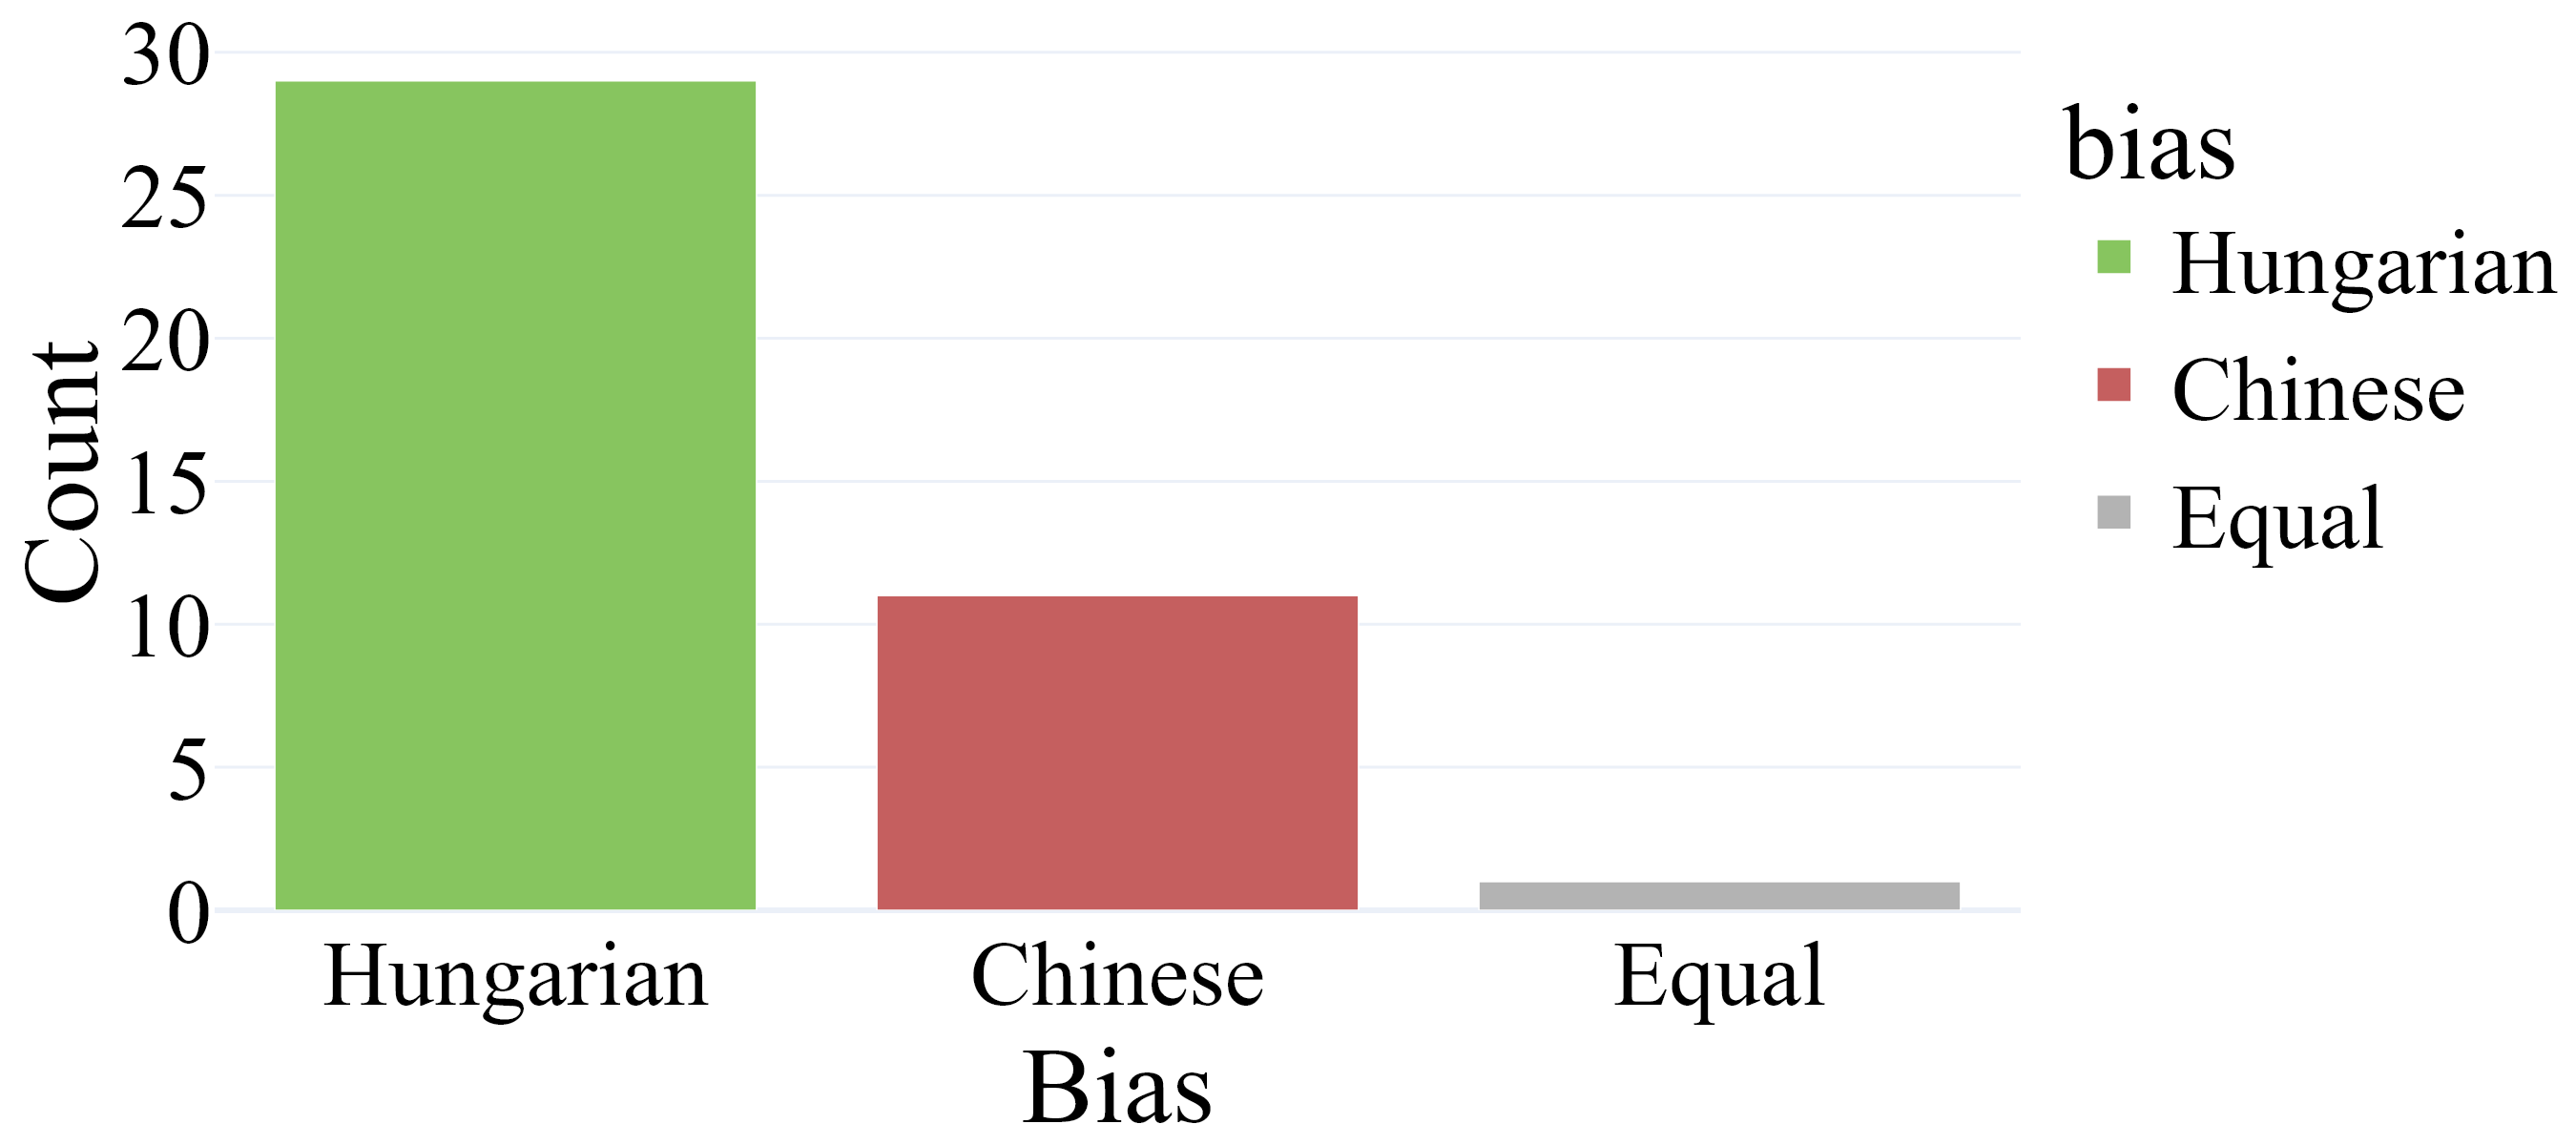
\includegraphics[width=\linewidth]{../bias_counts}
  \caption{Greater bias counts per occupation of Hungarian and Chinese ratings.}  
  \label{fig:bias_counts}
\end{figure}


%%%%%%%%%%%%%%%%%%%%%%%%%%%%%%%%%%%%%%%%%%%%%%%%%%%%%%%

\begin{figure*}[!ht]
  \centering
  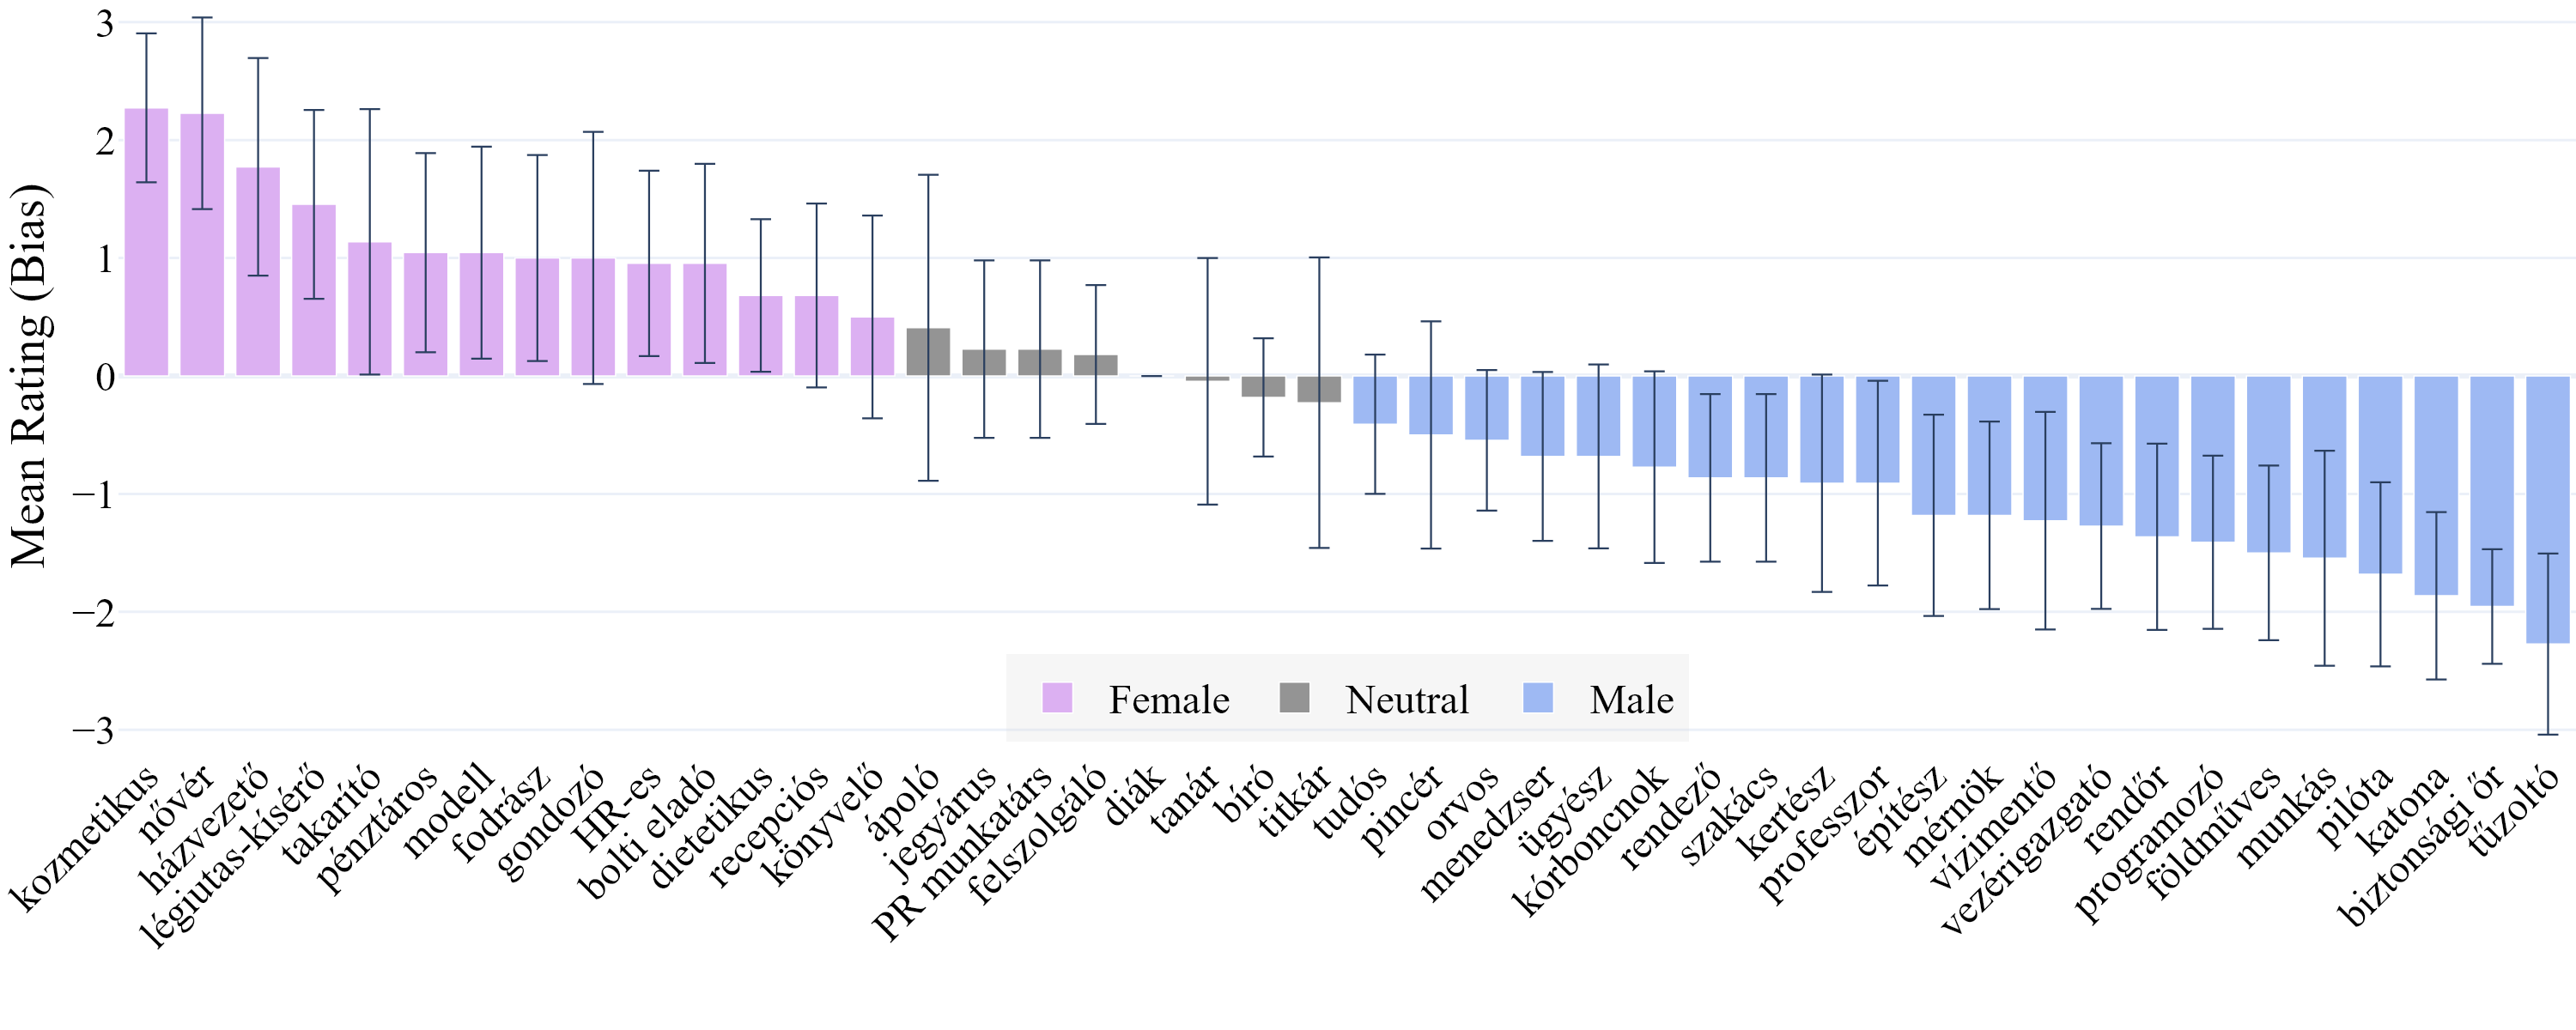
\includegraphics[width=\linewidth]{../occupations_hu}
  \caption{Mean ratings of occupational titles in Hungarian with standard deviations, significant gender bias highlighted -- \href{https://anonymous.4open.science/api/repo/occupational-gender-bias/file/occupations_hu.html?v=93359859}{explore the interactive plot}.}
  \label{fig:occupations_hu}
\end{figure*}

\begin{figure*}[tbp]
  \centering
  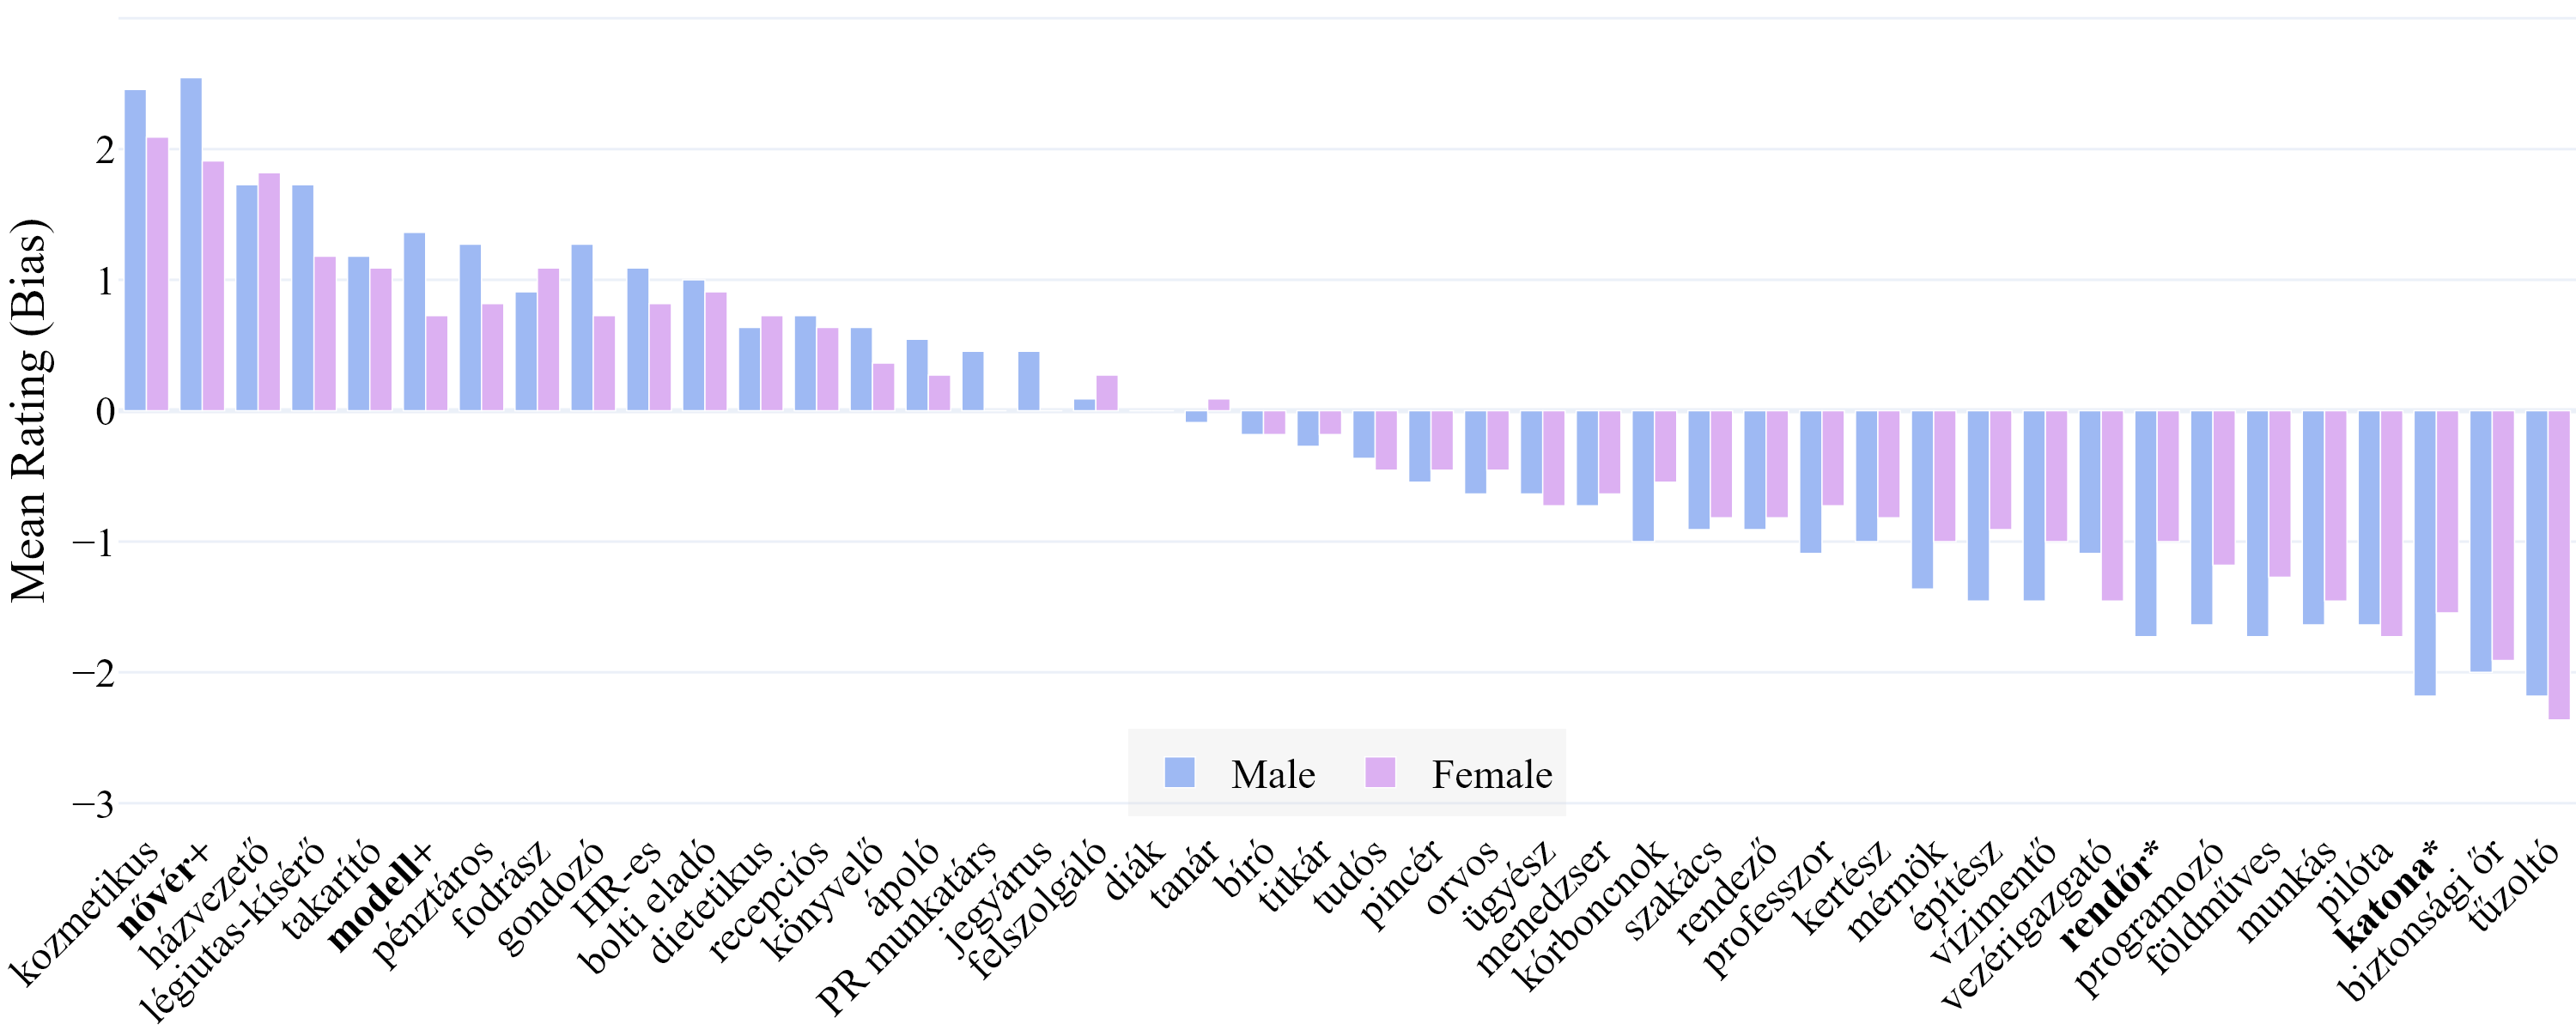
\includegraphics[width=\linewidth]{../occupations_hu_gender}
  \caption{Mean ratings of occupational titles in Hungarian by gender, significant differences highlighted (significant*, and marginally significant+ in \textbf{bold}) -- \href{https://anonymous.4open.science/api/repo/occupational-gender-bias/file/occupations_hu_gender.html?v=cf836c31}{explore the interactive plot}.}
  \label{fig:occupations_hu_gender}
\end{figure*}



\begin{figure*}[!ht]
  \centering
  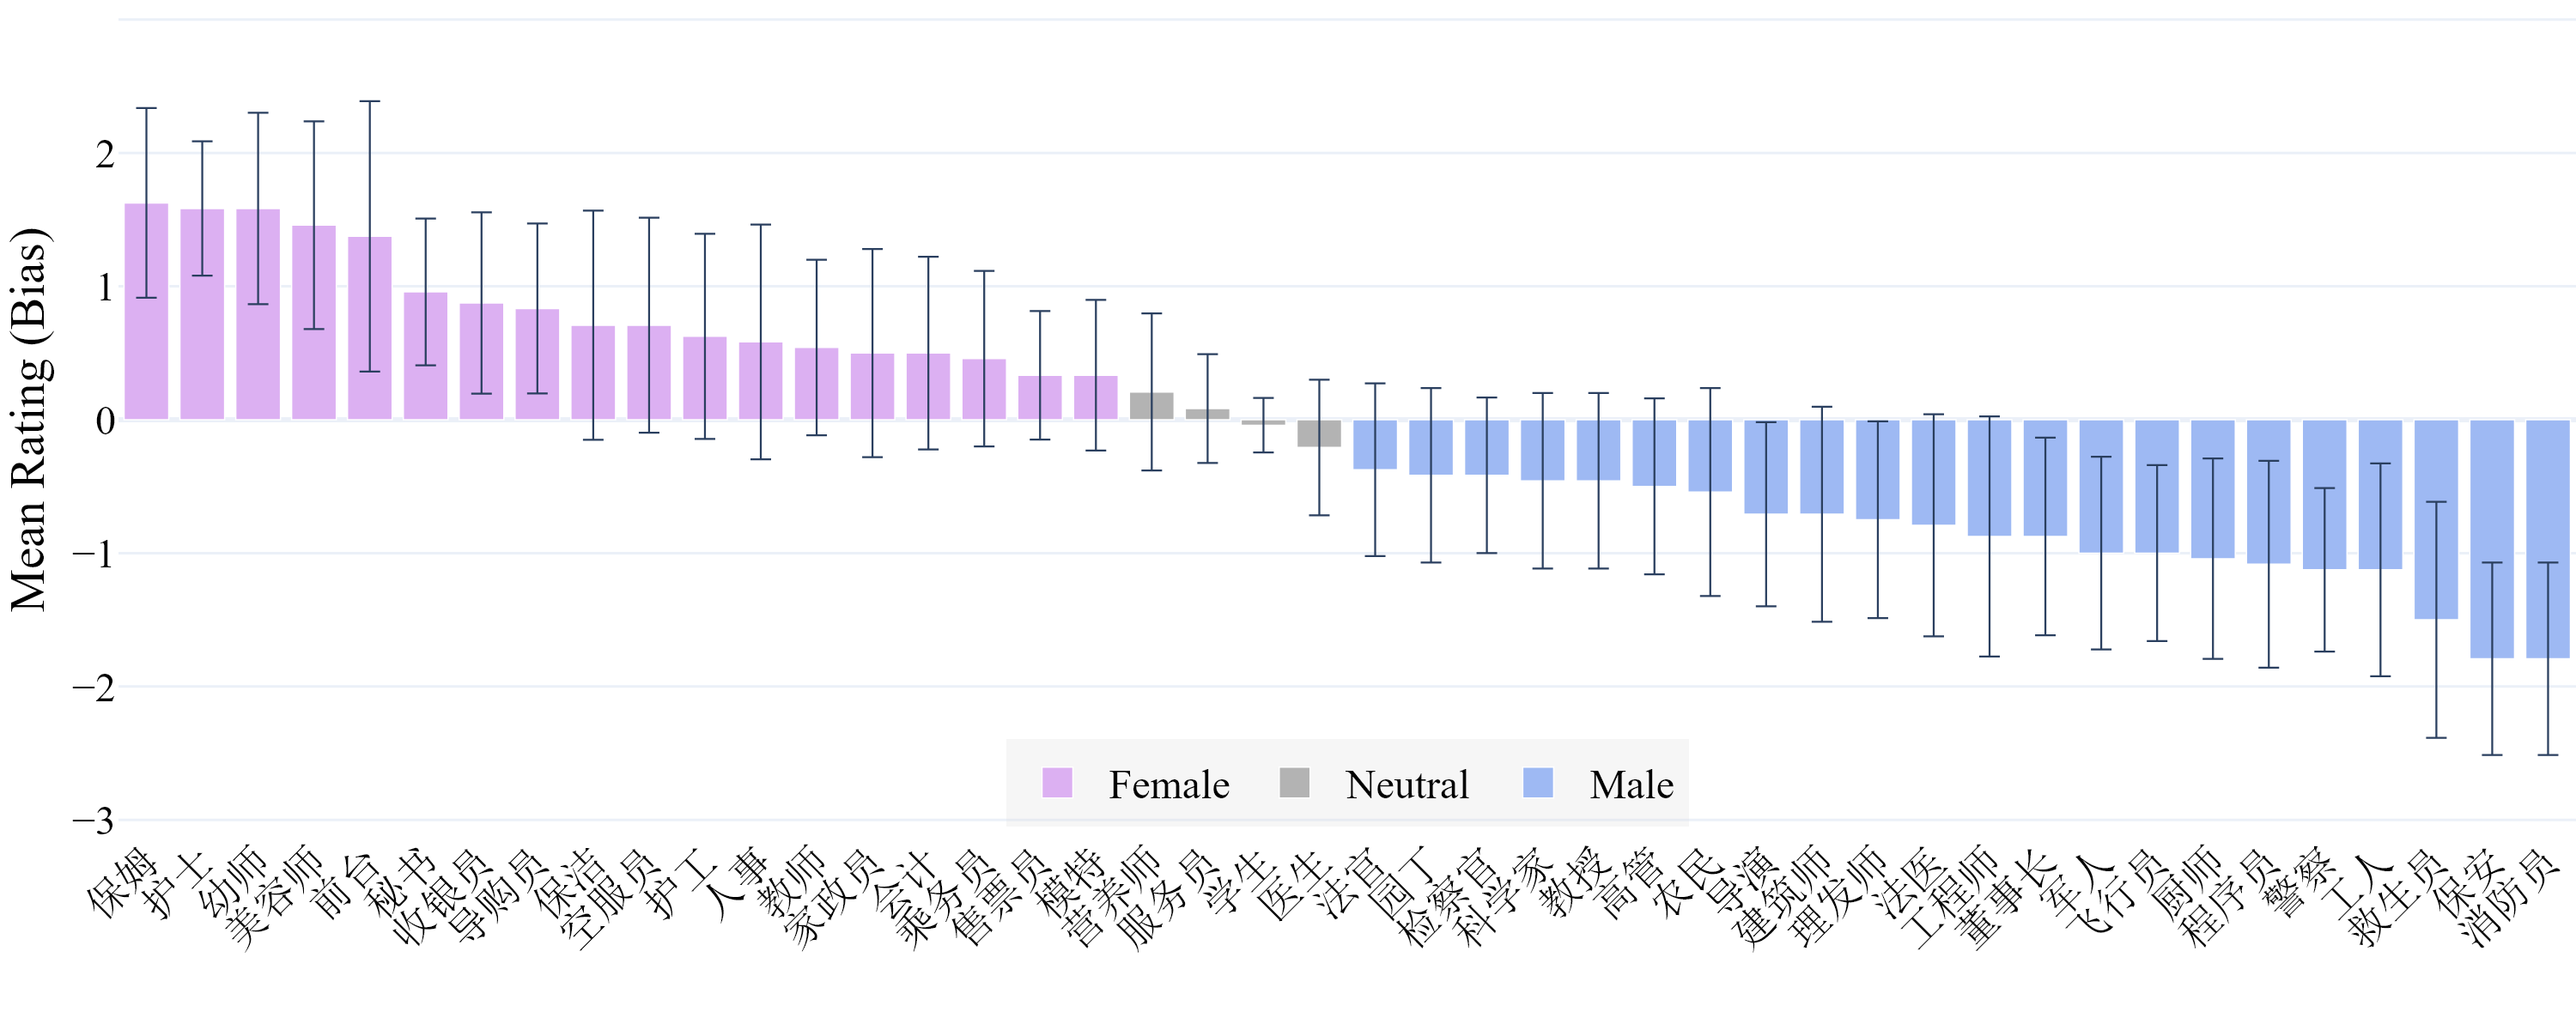
\includegraphics[width=\linewidth]{../occupations_zh}
  \caption{Mean ratings of occupational titles in Chinese with standard deviations, significant differences highlighted -- \href{https://anonymous.4open.science/api/repo/occupational-gender-bias/file/occupations_zh.html?v=9fe887c1}{explore the interactive plot}.}
  \label{fig:occupations_zh}
\end{figure*}

\begin{figure*}[tbp]
  \centering
  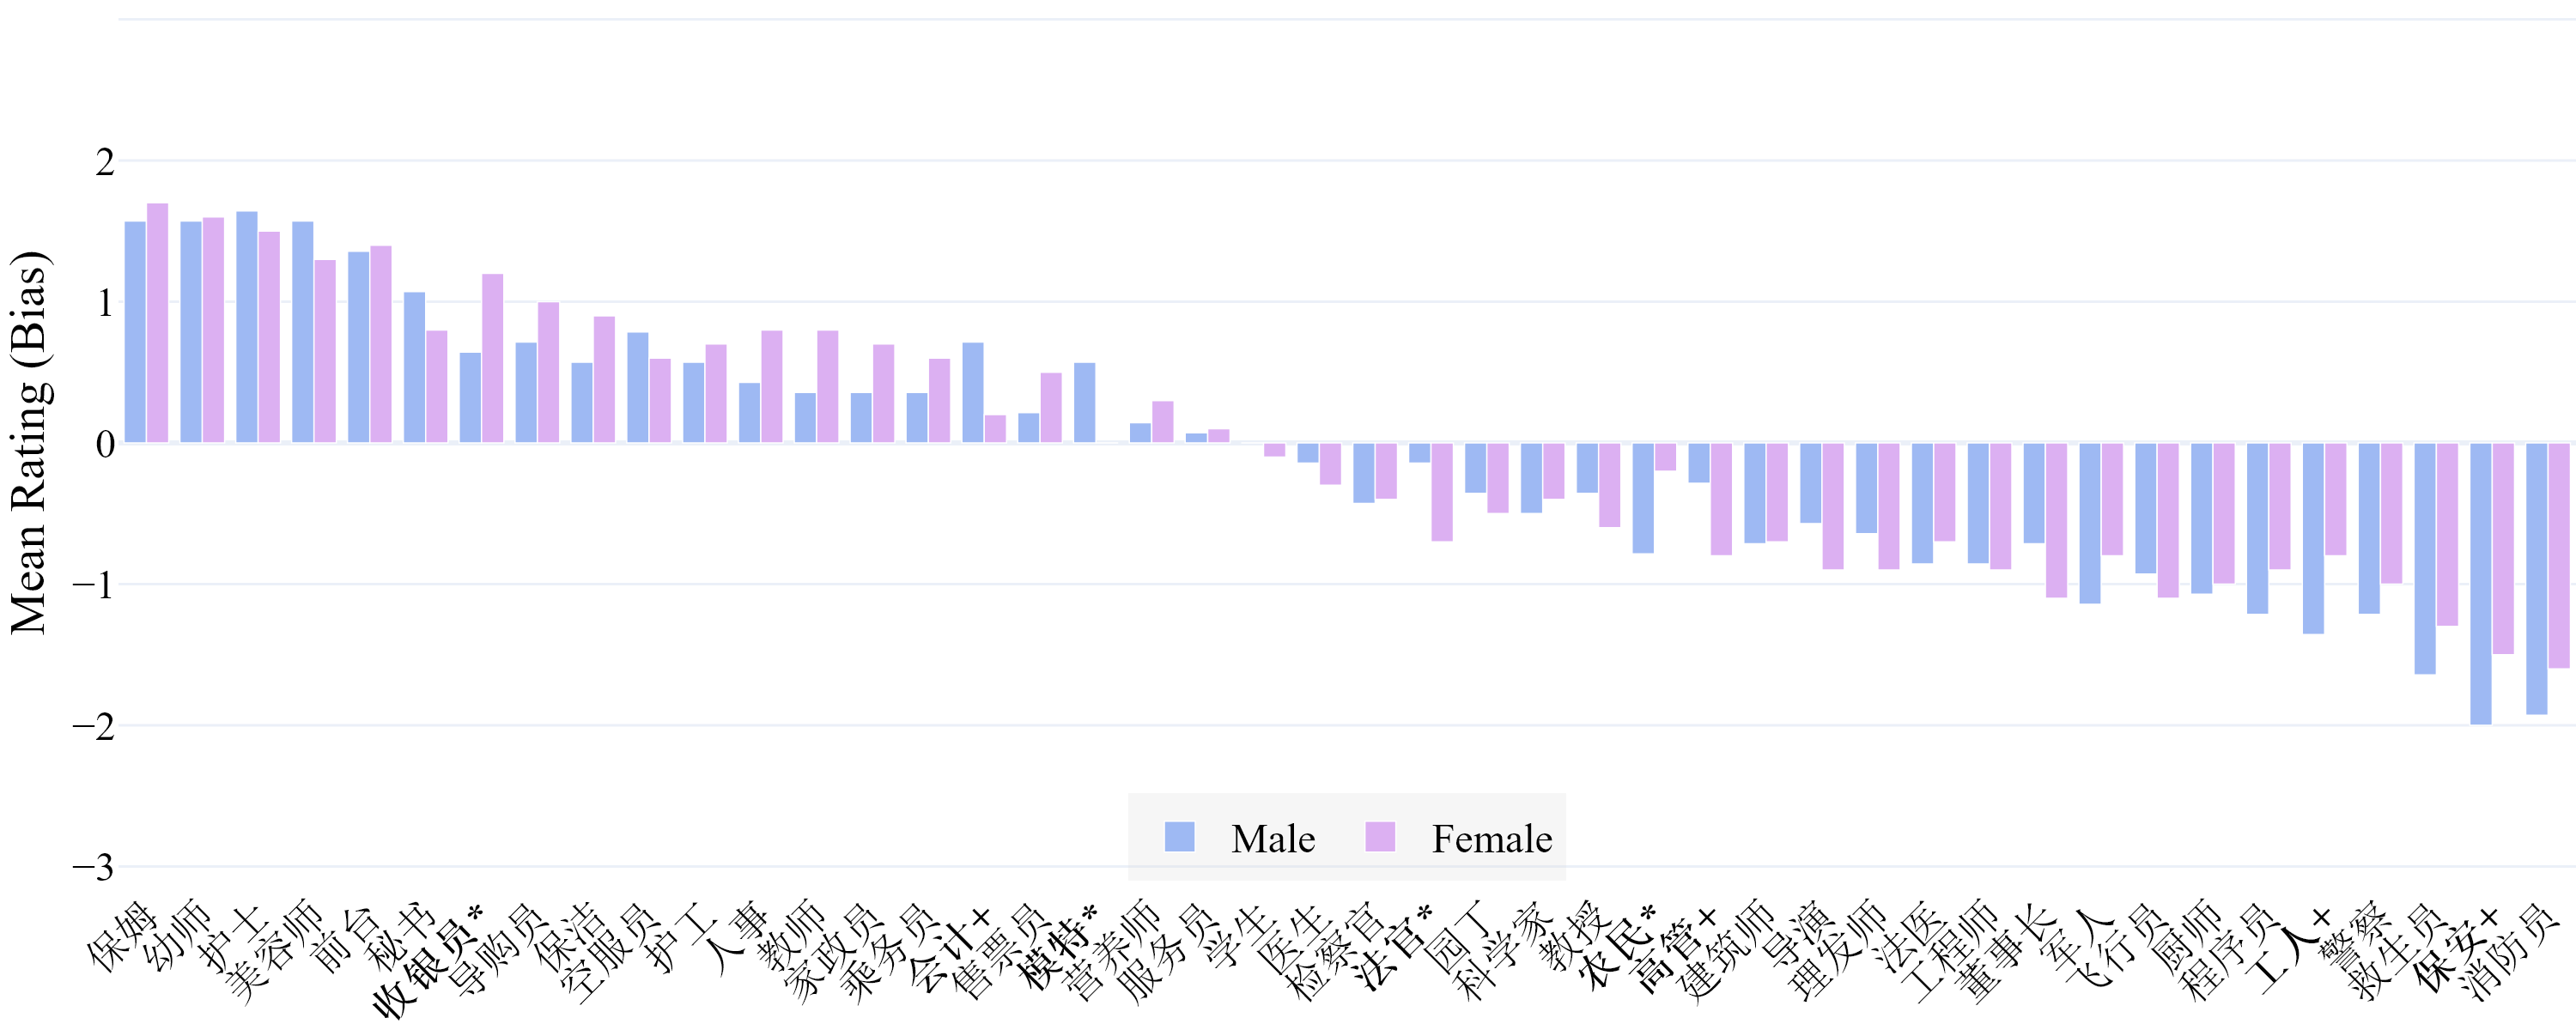
\includegraphics[width=\linewidth]{../occupations_zh_gender}
  \caption{Mean ratings of occupational titles in Chinese by gender, significant differences highlighted (significant*, and marginally significant+ in \textbf{bold}) -- \href{https://anonymous.4open.science/api/repo/occupational-gender-bias/file/occupations_zh_gender.html?v=99428eda}{explore the interactive plot}.}
  \label{fig:occupations_zh_gender}
\end{figure*}



\begin{figure*}[!ht]
  \centering
  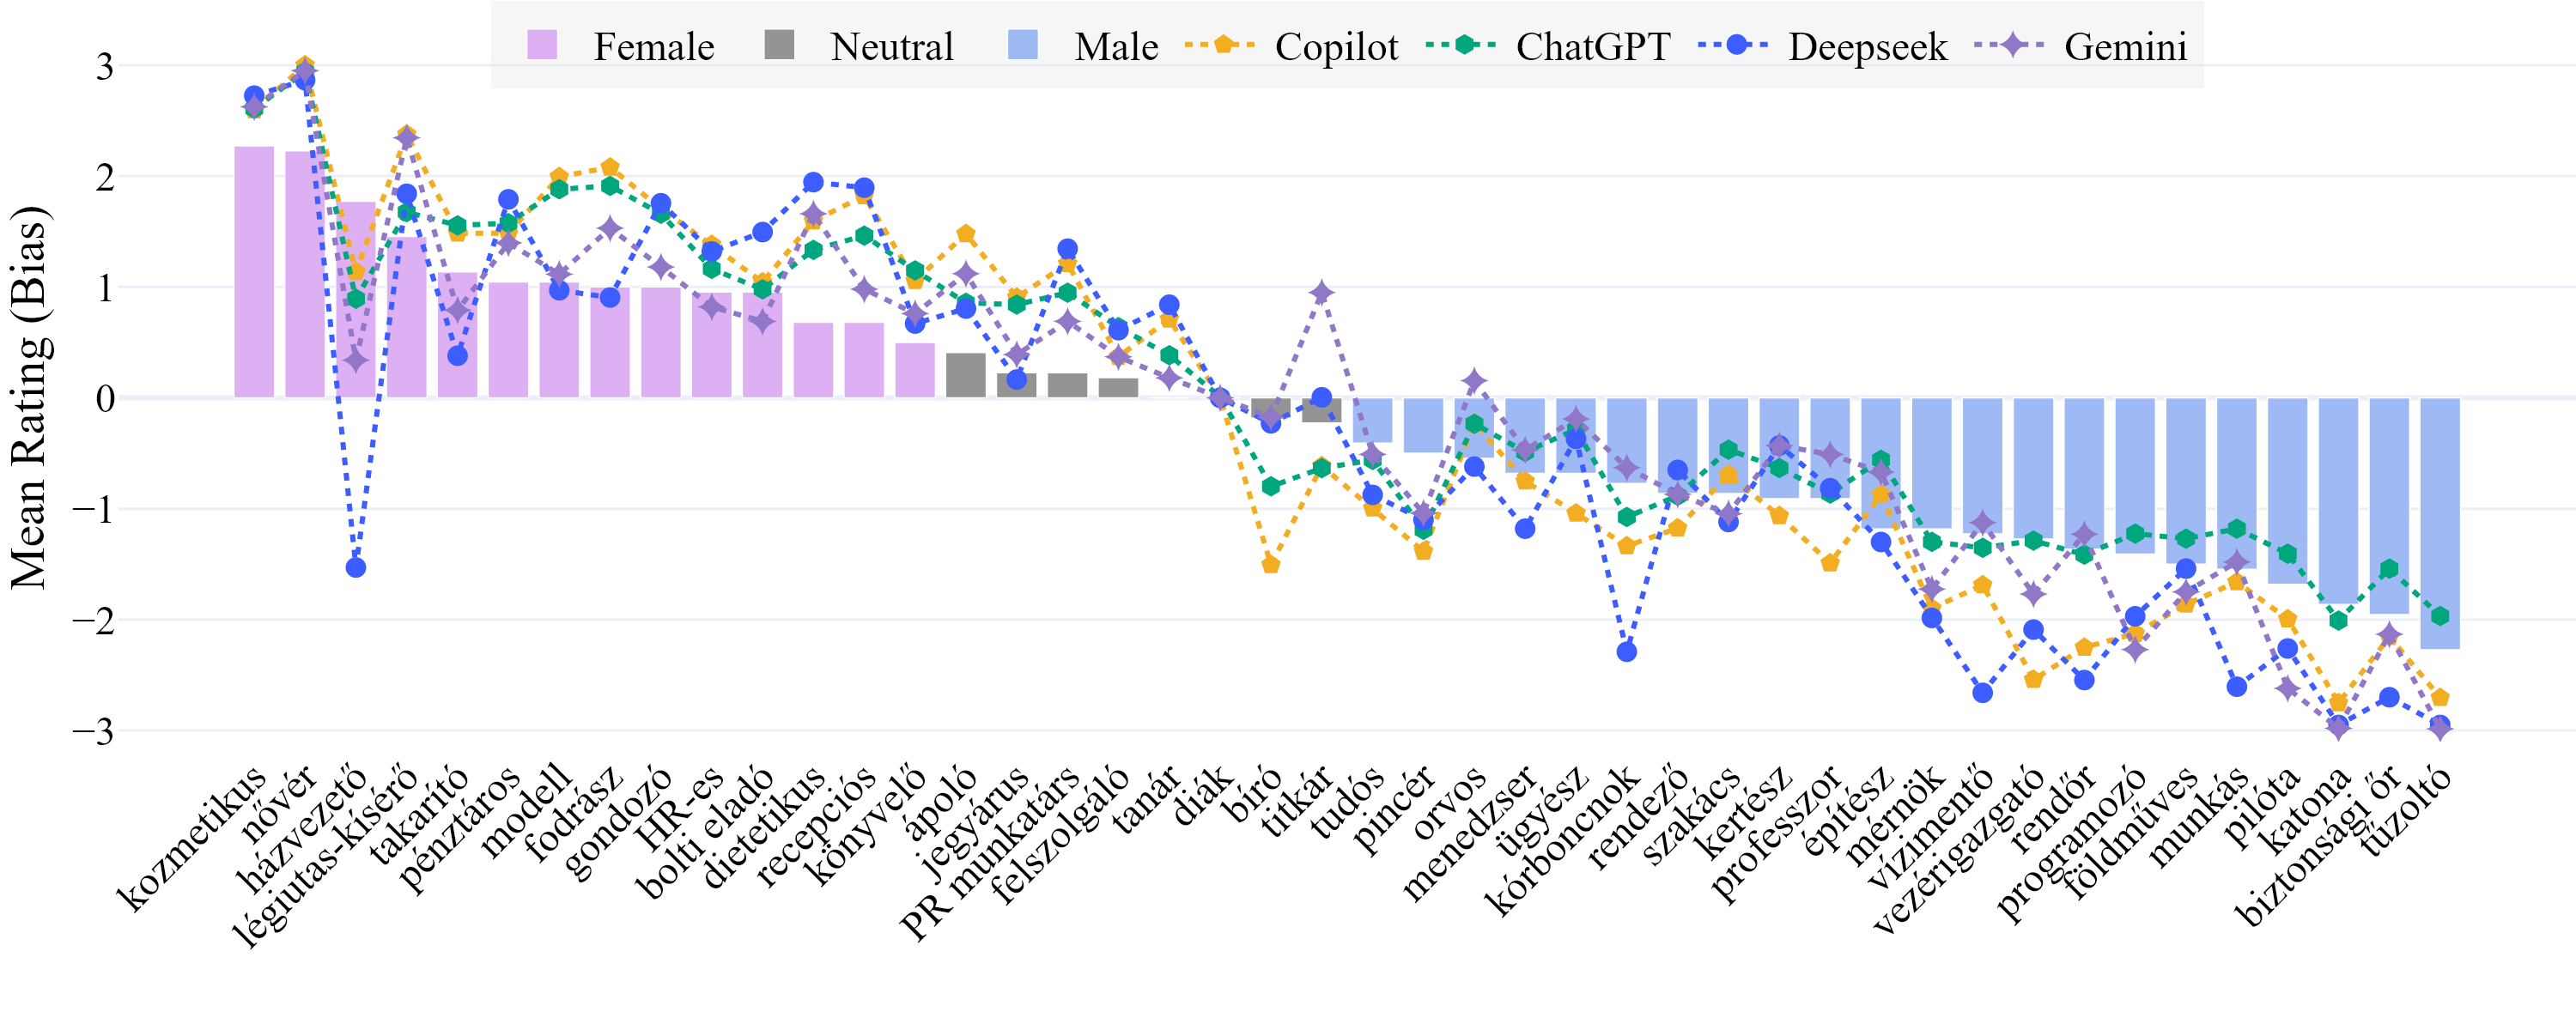
\includegraphics[width=\linewidth]{../occupations_hu_with_ai}
  \caption{AI ratings for Hungarian occupations \href{https://anonymous.4open.science/api/repo/occupational-gender-bias/file/occupations_hu_with_ai.html?v=87b2469e}{--- explore the interactive plot, click items in the legend to isolate}.}
  \label{fig:occupations_hu_with_ai}
\end{figure*}

\begin{figure*}[tbp]
  \centering
  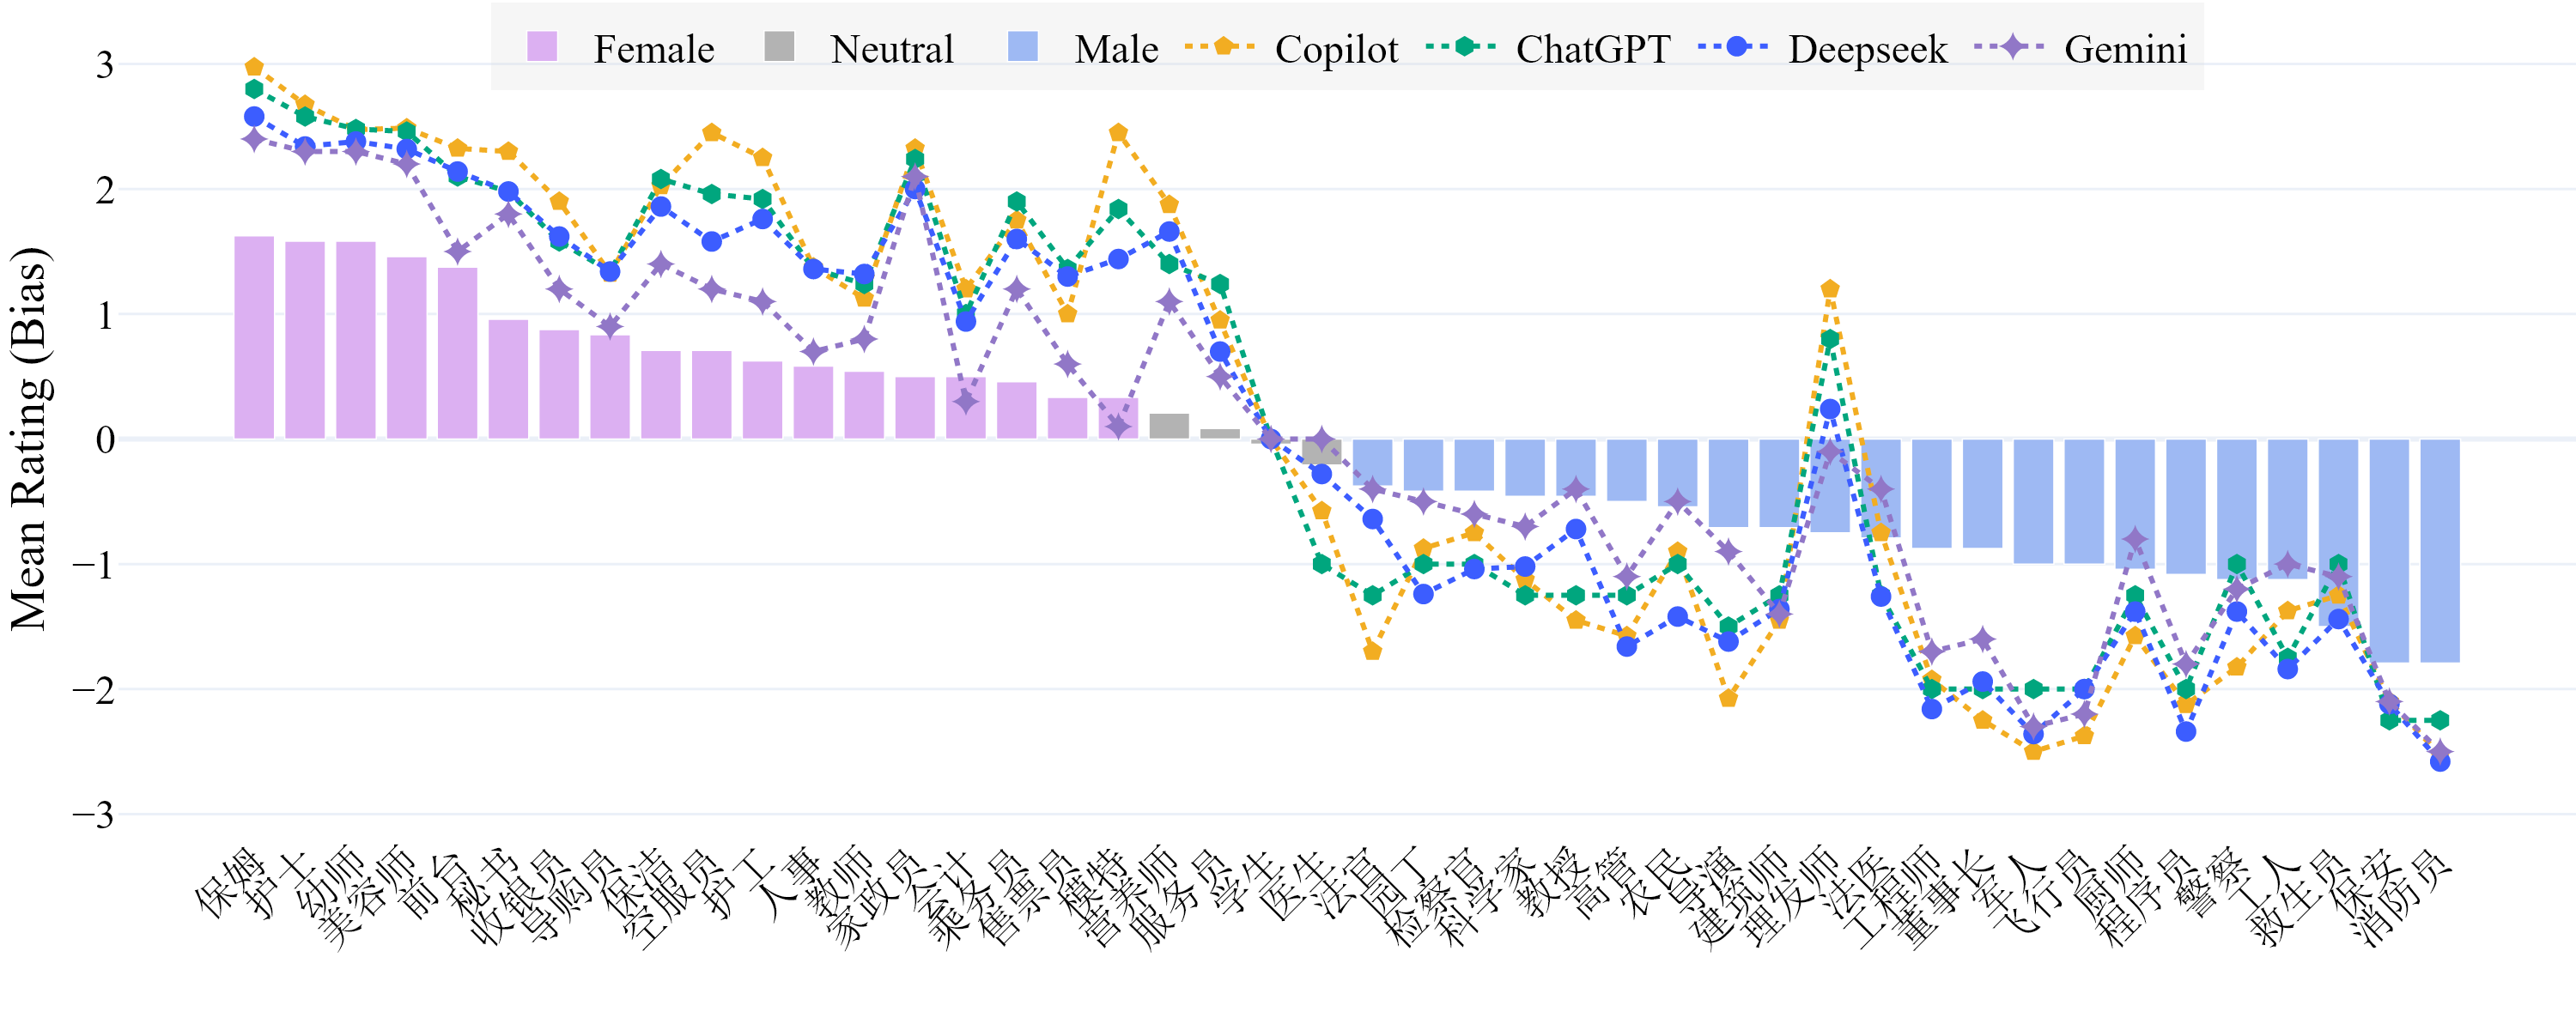
\includegraphics[width=\linewidth]{../occupations_zh_with_ai}
  \caption{AI ratings for Chinese occupations \href{https://anonymous.4open.science/api/repo/occupational-gender-bias/file/occupations_zh_with_ai.html?v=00fce30d}{--- explore the interactive plot, click items in the legend to isolate}.}
  \label{fig:occupations_zh_with_ai}
\end{figure*}



\begin{figure*}[!ht]
  \centering
  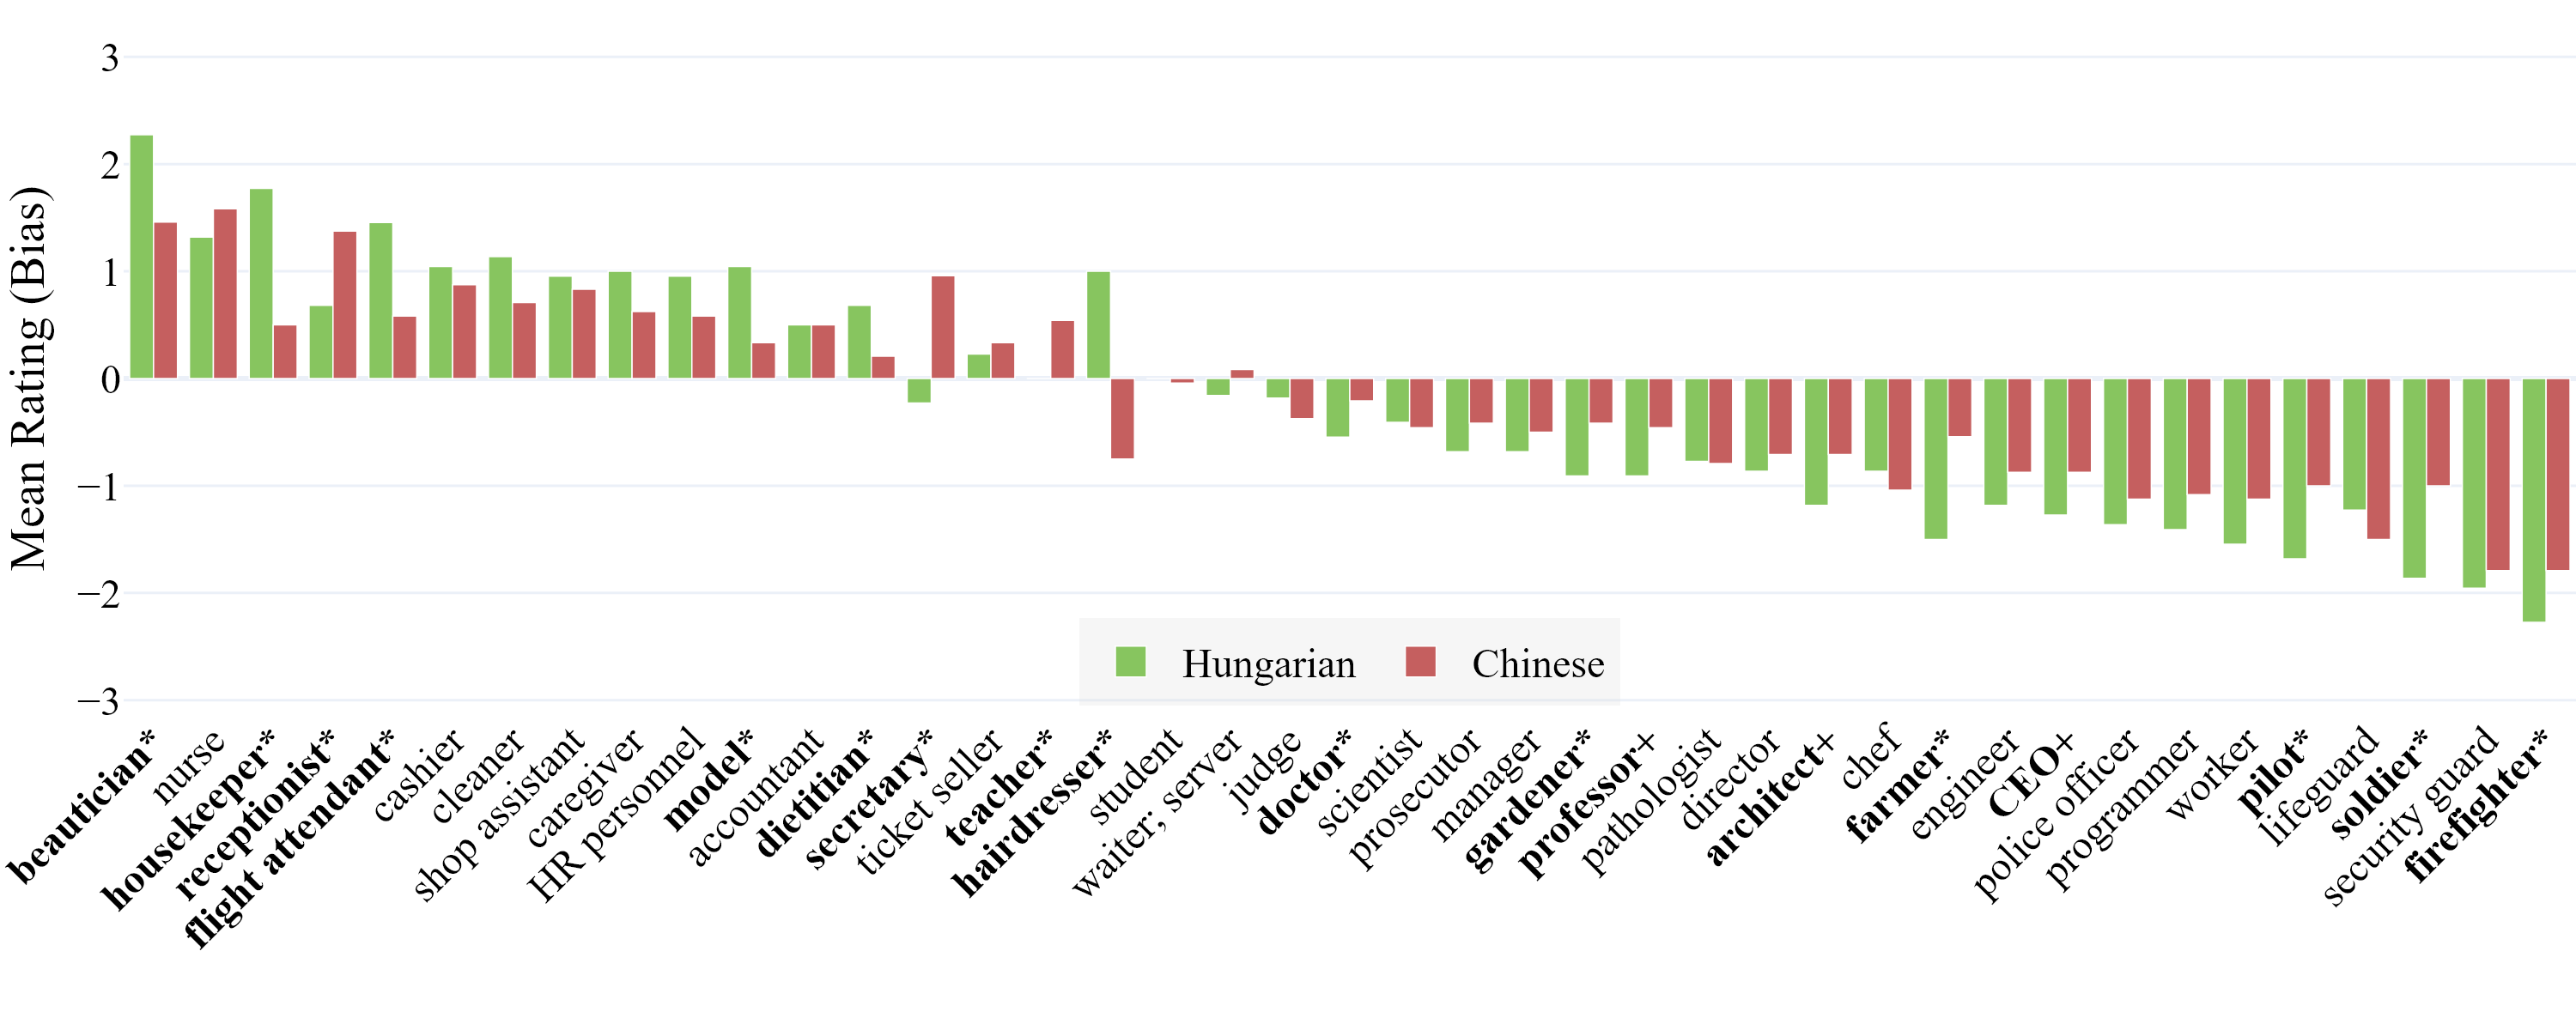
\includegraphics[width=\linewidth]{../occupations_comparison}
  \caption{Mean ratings of common occupational titles in Hungarian and Chinese (significant*, and marginally significant+ in \textbf{bold}) -- \href{https://anonymous.4open.science/api/repo/occupational-gender-bias/file/occupations_comparison.html?v=8cbb246d}{explore the interactive plot}.}
  \label{fig:occupations_comparison}
\end{figure*}










\end{document}
